\chapter{A-A TTP}
\localtableofcontents
\thispagestyle{plain}
\cleardoublepage

\section[BVR TTP]{BVR TTP --- BEYOND VISUAL RANGE TACTICS, TECHNIQUES, \break AND PROCEDURES}
\label{subsec:bvr}

\subsection[AR FUNDAMENTALS]{ACTIVE RADAR MISSILE FUNDAMENTALS}

\begin{figure}[htbp]
    \centering
    \begin{tikzpicture}[figstyle]
        % help lines
        % \draw[help lines] (0,-10) grid (100,10);

        % MISSILE
        \coordinate (A_missile) at (0,0);
        \coordinate (B_missile) at (30,10);
        \coordinate (C_missile) at (60,3);
        \coordinate (D_missile) at (80,0);

        \draw[thick, ->]
        (A_missile) .. controls ($(A_missile)+(20,0)$) and ($(B_missile)+(-10,0)$) .. 
        (B_missile) .. controls ($(B_missile)+(5,0)$) and ($(C_missile)+(-10,2.5)$) ..
        (C_missile);
        \draw[dotted, thick, ->] 
        (C_missile) .. controls ($(C_missile)+(10,-2.5)$) and ($(D_missile)+(-5,0)$) ..
        (D_missile);

        \node[above] at (A_missile) {\titlefont A};
        \node[above] at (B_missile) {\titlefont B};
        \node[above] at (C_missile) {\titlefont C};
        \node[above] at (D_missile) {\titlefont D};

        % FIGHTER
        \coordinate (A_fighter) at (A_missile);
        \coordinate (C_fighter) at ($(A_fighter)+(20,0)$);
        \coordinate (D_fighter) at ($(C_fighter)+(-5,-5)$);

        \node[
            anchor=east,
        ] (fig_A_fighter) at (A_fighter) {
            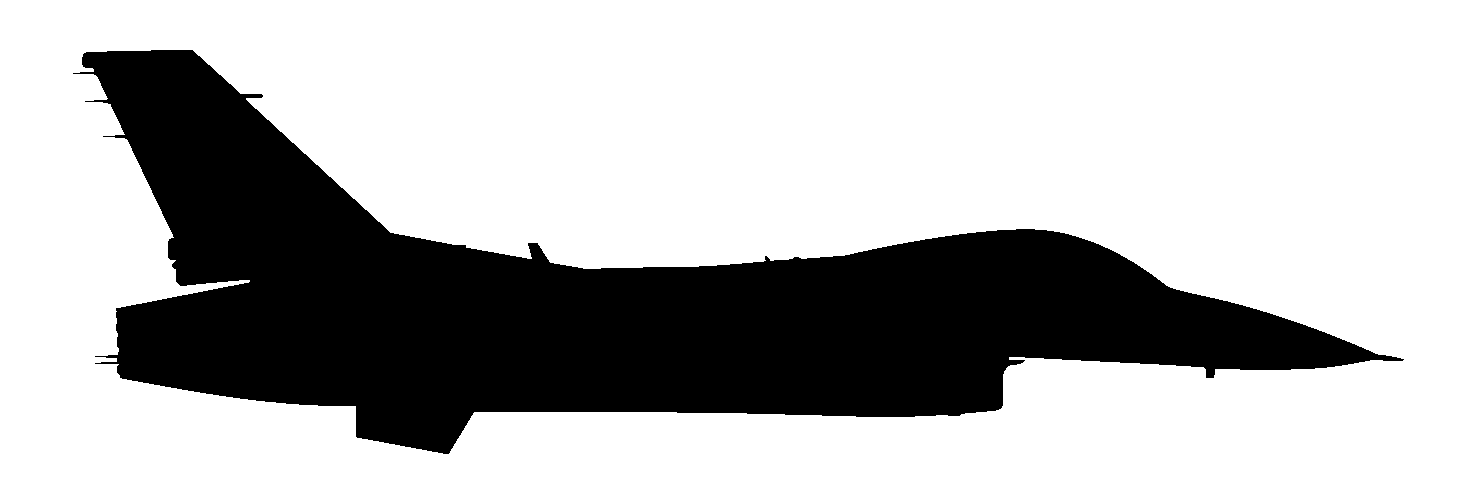
\includegraphics[
                width=7.5mm,
            ]{diagrams/aircraft/silhouette_f16_side.pdf}
        };

        \draw[ultra thick, ->] 
        (A_fighter) -- 
        (C_fighter) .. controls ($(C_fighter)+(5,0)$) and ($(C_fighter)+(5,-5)$) .. 
        ($(C_fighter)+(0,-5)$) --
        (D_fighter);

        \node[above right] at (C_fighter) {\titlefont C};
        \node[left] at (D_fighter) {\titlefont D};

        % BANDIT
        \coordinate (A_bandit) at (100,0);
        \coordinate (C_bandit) at (85,0);
        \coordinate (D_bandit) at (D_missile);

        \draw[ultra thick, ->] 
        (A_bandit) -- 
        (D_bandit);

        \node[above] at (A_bandit) {\titlefont A};
        \node[above] at (C_bandit) {\titlefont C};

        \filldraw[red] (D_bandit) circle (2pt);

        % Distance lines
        \draw[thin, <->]
        ($(C_fighter)+(0,-12.5)$) -- node[pos=0.5, above]{\small\titlefont R\textsubscript{A-POLE}}
        ($(C_bandit)+(0,-12.5)$);
        \draw[thin, <->]
        (15,-20) -- node[pos=0.5, above]{\small\titlefont R\textsubscript{F-POLE}}
        ($(D_missile)+(0,-20)$);
        \draw[thin, <->]
        ($(A_missile)+(0,-27.5)$) -- node[pos=0.5, above]{\small\titlefont R\textsubscript{LAUNCH}}
        ($(A_bandit)+(0,-27.5)$);

        \draw[thin]
        ($(C_fighter)+(0,-2.5)$) -- ($(C_fighter)+(0,-15)$)
        ($(C_bandit)+(0,-2.5)$) -- ($(C_bandit)+(0,-15)$)
        ($(D_fighter)+(0,-2.5)$) -- (15,-22.5)
        ($(D_missile)+(0,-2.5)$) -- ($(D_missile)+(0,-22.5)$)
        ($(A_missile)+(0,-2.5)$) -- ($(A_missile)+(0,-30)$)
        ($(A_bandit)+(0,-2.5)$) -- ($(A_bandit)+(0,-30)$);

    \end{tikzpicture}
    \caption{Side-on view of a generic AIM-120 employment profile}
    \label{fig:aa_weap:bvr:aim120profile}
    % TODO: silhouettes?
\end{figure}

\begin{tcoloritemize}
    \blueitem[AIM-120 \break Employment \break Profile]
    \Cref{fig:aa_weap:bvr:aim120profile} shows the trajectories of fighter, bandit \& missile for a generic AIM-120 employment profile
    including the following phases

    \begin{itemize}
        \item \textbf{A --- Launch / Boost Phase}
        \item \textbf{B --- Mid-Course Phase}
        \item \textbf{C --- Acquisition}
        \item \textbf{D --- Intercept}
    \end{itemize}
    \blueitem[Launch / Boost Phase]
    \textbf{Boost}

    \begin{itemize}
        \item Motor only fires for initial seconds of flight 
        \item After burnout missile \textbf{\underline{cannot gain energy}}
    \end{itemize}

    \textbf{Lofting} 

    \begin{itemize}
        \item To reach longer ranges missile ``lofts'' itself to conserve energy \& optimize trajectory
        \item Pilot can manually loft by raising the nose 20-30 deg prior to launch
    \end{itemize}
    \blueitem[Mid-Course Phase]
    \textbf{Missile flies using internal IMU}

    \begin{itemize}
        \item Receives periodic datalink updates
        \item Will fly to last updated target position if DL lost
    \end{itemize}
    \blueitem[Acquisition \& MPRF ``Active'' Phase]
    \textbf{Missile radar turns on once close to target location}
    \begin{itemize}
        \item Seeker in MPRF (Medium Pulse Repetition Frequency) mode 
        \item Locks on to closest / best target
    \end{itemize}
    \blueitem[Terminal Phase \& Intercept]
    \textbf{Once missile seeker has acquired target}
    \begin{itemize}
        \item Flies PNG intercept trajectory
        \item Requires no further DL support, fighter can turn away from the bandit
    \end{itemize}
\end{tcoloritemize}

\cautionbox{
    \textbf{Do NOT employ AIM-120 without clear avenue-of-fire} 
    \begin{itemize}
        \item AIM-120 has NO IFF functionality
    \end{itemize}
}

\subsubsection{TACTICAL CONSIDERATIONS}
\label{subsec:bvr:tacticalconsideration}
% \label{subsec:aim120:tactics}
\begin{tcoloritemize}
    \blueitem[Range Definitions]
    \textbf{Fighter-bandit distance} can be measured at different points during the timeline

    \begin{itemize}
        \item \textbf{R\textsubscript{Launch}} --- distance at launch
        \item \textbf{R\textsubscript{A-Pole}} --- distance when missile goes active
        \item \textbf{R\textsubscript{F-Pole}} --- distance at impact
    \end{itemize}
    
    These are also illustrated in \cref{fig:aa_weap:bvr:aim120profile}.
    \blueitem[Maximizing Launch Range / Energy]
    \textbf{Why?}
    \begin{itemize}
        \item Ability to launch at longer ranges forces bandit defensive
        \item Bandit may not be able to counter-launch
        \item Higher launch energy increases P\textsubscript{intercept} %probability of intercept
    \end{itemize}
    \textbf{How?}
    \begin{itemize}
        \item \textbf{High velocity} --- increases kinetic energy 
        \item \textbf{High altitude} --- increases potential energy, reduces drag
    \end{itemize}
    \blueitem[Maximizing \break F-Pole Range]
    \textbf{Why?}
    \begin{itemize}
        \item Less likely to enter bandit launch envelope
        \item More time/range to launch 2nd missile if necessary
    \end{itemize}
    \textbf{How?}
    \begin{itemize}
        \item \textbf{Crank} --- turn 45-60 degrees away from bandit to reduce closure rate, maintain radar contact
        \item \textbf{Dive} --- reduces threat missile envelope
    \end{itemize}
    \blueitem[Flowing Cold]
    \textbf{Why?}
    \begin{itemize}
        \item Missile requires no support once active
        \item Defend against unknown missile launches
        \item Maximize F-pole range further
    \end{itemize}
    \textbf{How?}
    \begin{itemize}
        \item \textbf{Turn} --- Away from bandit / threat
        \item \textbf{Dive} --- if necessary, reduces threat missile envelope 
    \end{itemize}
    \blueitem[Effect of Bandit Maneuvers]
    As evident in \cref{fig:aa_weap:bvr:aim120profile}, 
   \textbf{R\textsubscript{Launch}} is significantly greater than the distance travelled by the missile
    \begin{itemize}
        \item \textbf{DLZ calculated based off \underline{both} fighter \underline{and} bandit velocity/altitude}
        \item Bandit can significantly change missile envelope by reducing closure rate / altitude
        \item Post-launch bandit maneuvers can result in missile not having energy to intercept
    \end{itemize}
\end{tcoloritemize}

\clearpage

\subsubsection{FIGHTER MANEUVERS}

\begin{tcoloritemize}
    \blueitem[Crank]
    Fighter turns \textbf{45-60 deg} away from threat 

    \begin{itemize}
        \item reduces closure while maintaining radar track
        \item typically used post-launch
    \end{itemize}
    
    Reference \cref{fig:aa_weap:bvr:fightermaneuver:crank}
    \blueitem[Notch]
    Fighter turns \textbf{70-110 deg} away from threat

    \begin{itemize}
        \item minimizes relative velocity to break hostile pulse-doppler radar track
        \item increases angular motion, forcing missile to maneuver and expend energy
    \end{itemize}
    
    Reference \cref{fig:aa_weap:bvr:fightermaneuver:notch}
    \blueitem[Go Cold]
    Fighter turns \textbf{away} from threat

    \begin{itemize}
        \item used to kinematically defeat threat missiles
    \end{itemize}
    
    Reference \cref{fig:aa_weap:bvr:fightermaneuver:cold}
\end{tcoloritemize}

\begin{figure}[htbp]
    \centering
    \begin{subfigure}[b]{0.3\linewidth}
        \centering
        \begin{tikzpicture}[figstyle]
            % FIGHTER
            \node[
                anchor=north,
                yshift=1mm,
            ] (fighter) at (0,0) {
                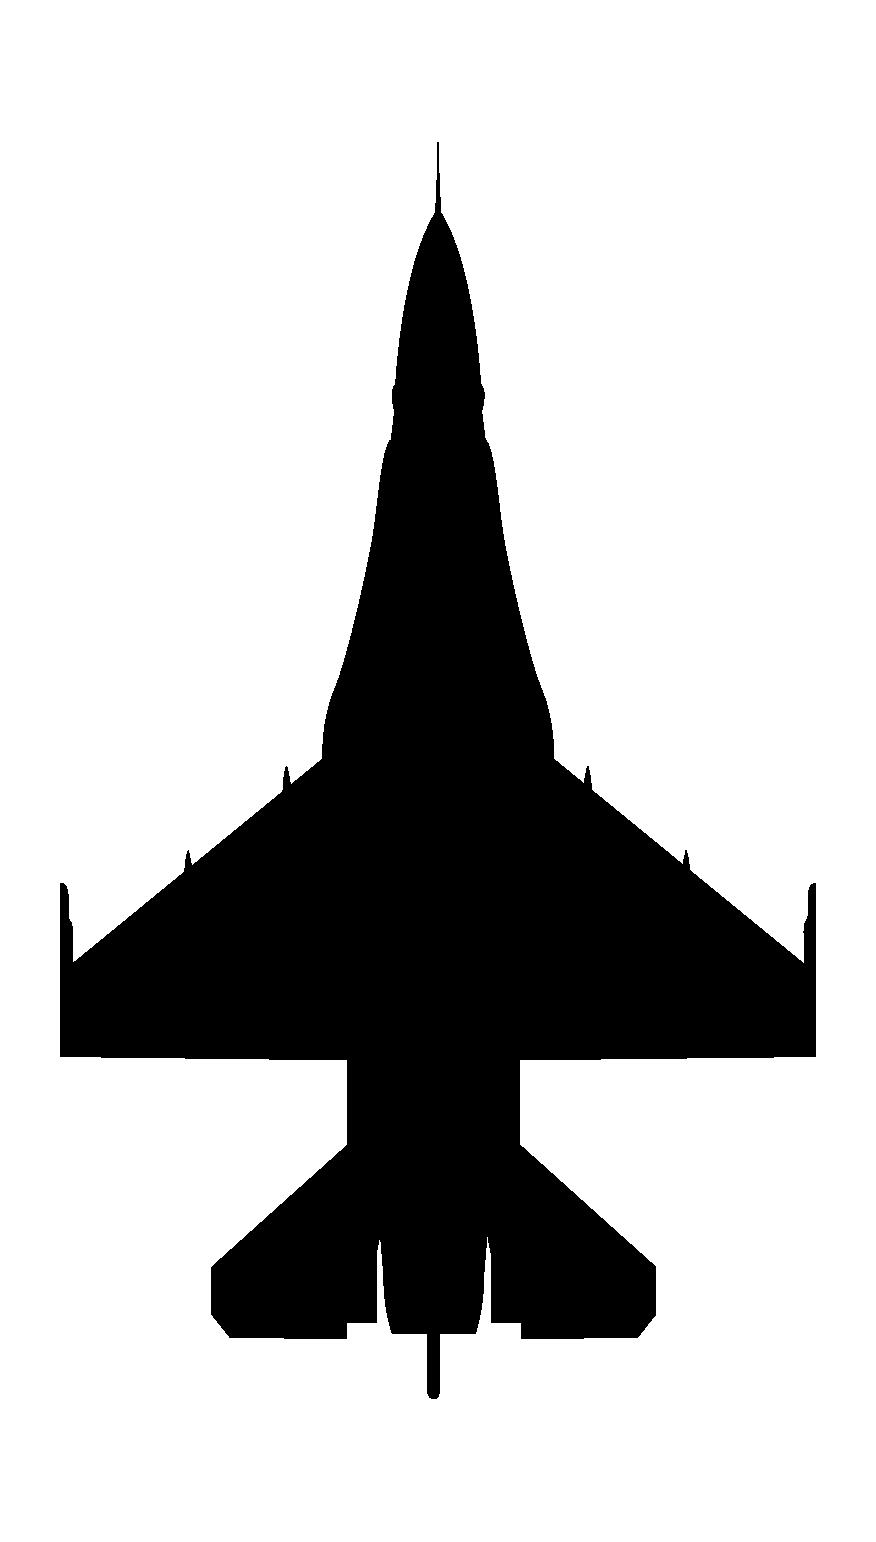
\includegraphics[
                    width=7.5mm,
                ]{diagrams/aircraft/silhouette_f16_top.pdf}
            };
            \draw[rounded corners, ->] 
            (0,0) -- (0,5) -- +(30:15) node[rotate=-60, anchor=south, yshift=-1mm]{
                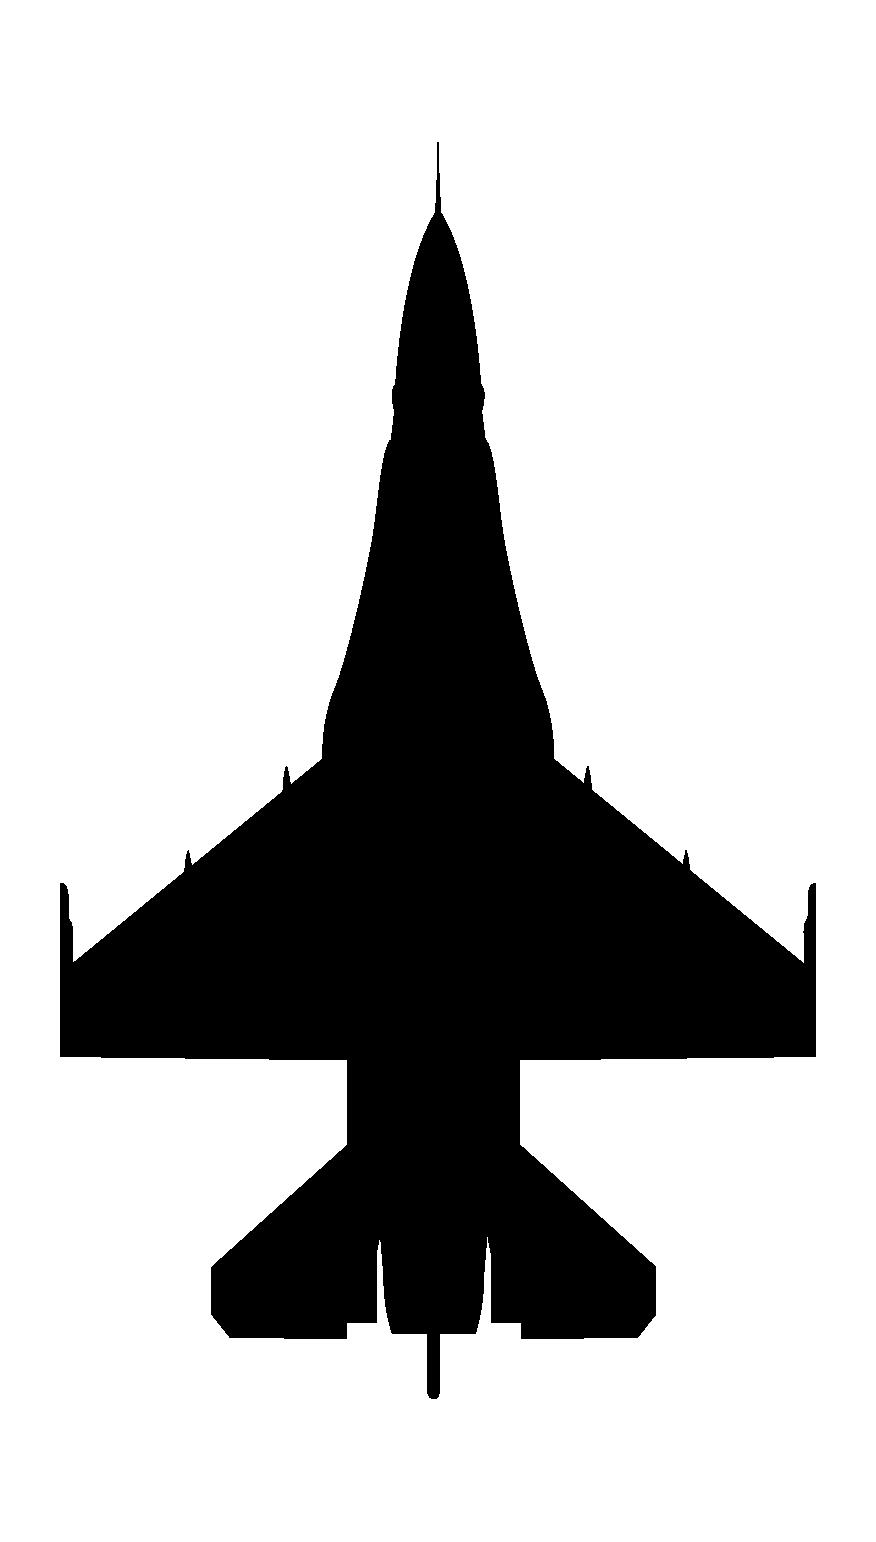
\includegraphics[
                width=7.5mm,
            ]{diagrams/aircraft/silhouette_f16_top.pdf}};
    
            % BANDIT
            \draw[rounded corners, ->] 
            (0,35) -- (0,25);
    
            % help line
            \draw[thin, dashed] 
            (0,25) -- (0,5);
    
            \draw[thin]
            (0,15) arc (90:30:10) node[pos=0.15, above right]{\small\titlefont 45-60$^\circ$};
    
        \end{tikzpicture}
        \caption{Crank}
        \label{fig:aa_weap:bvr:fightermaneuver:crank}
    \end{subfigure}
    \begin{subfigure}[b]{0.3\linewidth}
        \centering
        \begin{tikzpicture}[figstyle]
            % FIGHTER
            \node[
                anchor=north,
                yshift=1mm,
            ] (fighter) at (0,0) {
                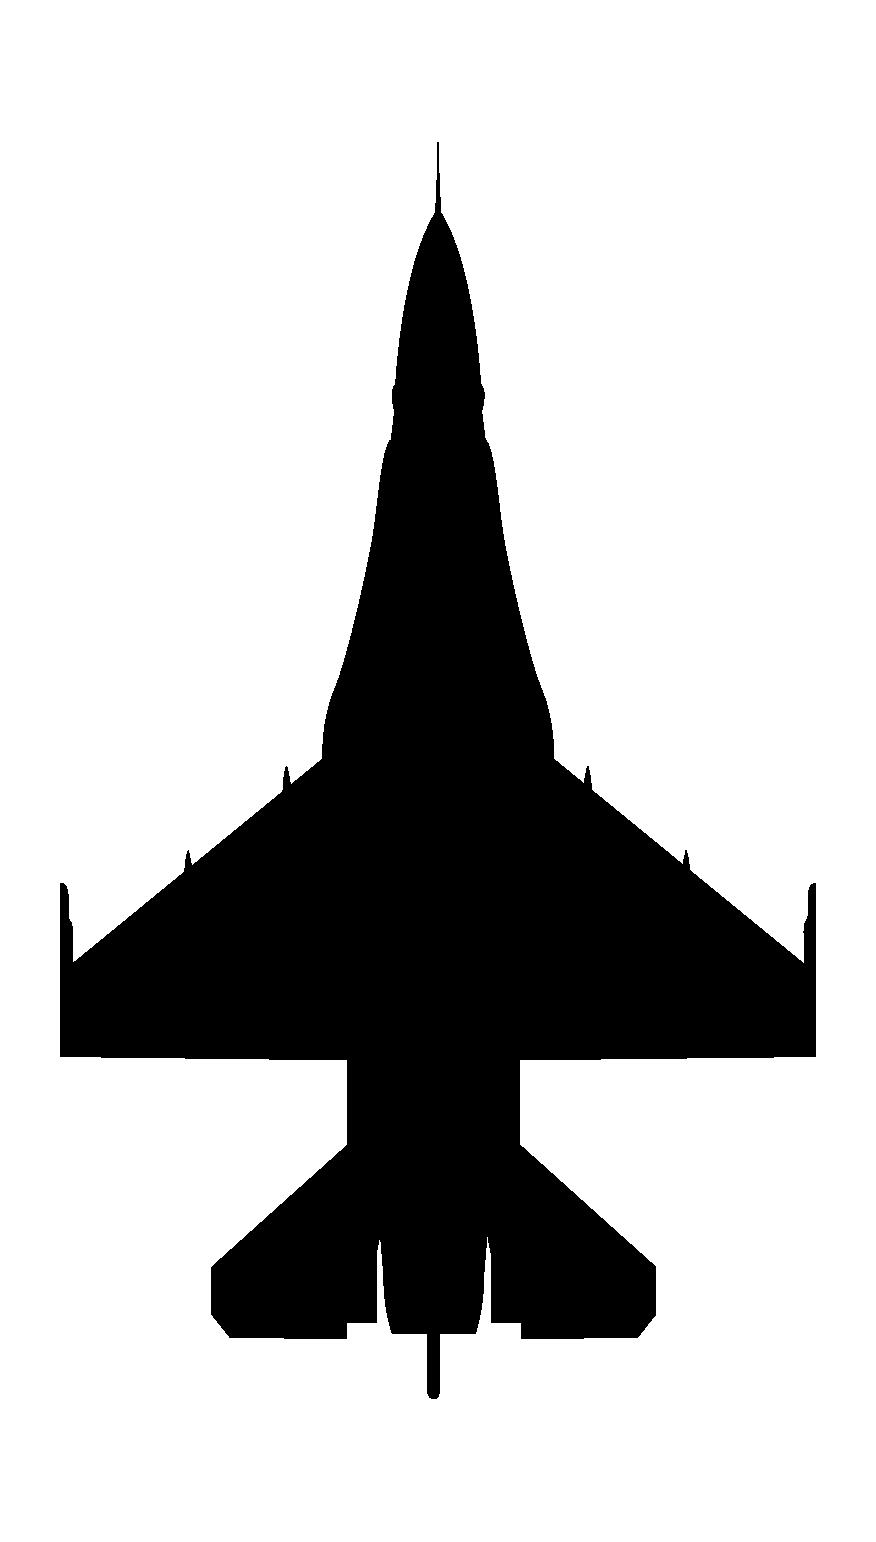
\includegraphics[
                    width=7.5mm,
                ]{diagrams/aircraft/silhouette_f16_top.pdf}
            };
            \draw[rounded corners, ->] 
            (0,0) -- (0,5) -- +(0:15) node[rotate=-90, anchor=south, yshift=-1mm]{
                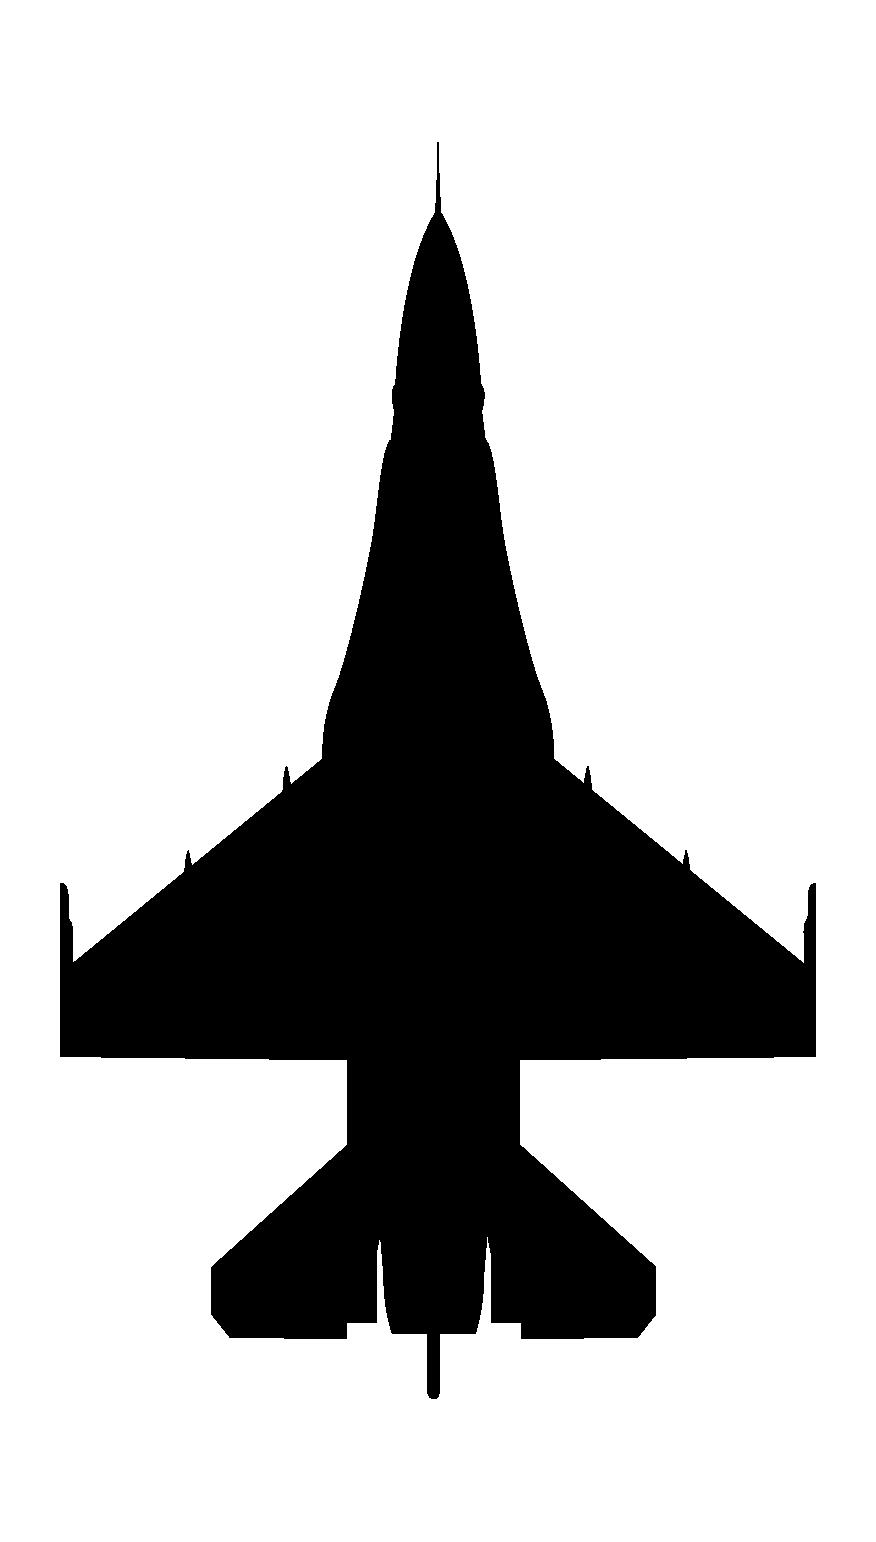
\includegraphics[
                width=7.5mm,
            ]{diagrams/aircraft/silhouette_f16_top.pdf}};
    
            % BANDIT
            \draw[rounded corners, ->] 
            (0,35) -- (0,25);
    
            % help line
            \draw[thin, dashed] 
            (0,25) -- (0,5);
    
            \draw[thin]
            (0,15) arc (90:0:10) node[pos=0.5, above right]{\small\titlefont 70-110$^\circ$};
    
        \end{tikzpicture}
        \caption{Notch}
        \label{fig:aa_weap:bvr:fightermaneuver:notch}
    \end{subfigure}
    \begin{subfigure}[b]{0.3\linewidth}
        \centering
        \begin{tikzpicture}[figstyle]
            % FIGHTER
            \node[
                anchor=north,
                yshift=1mm,
            ] (fighter) at (0,0) {
                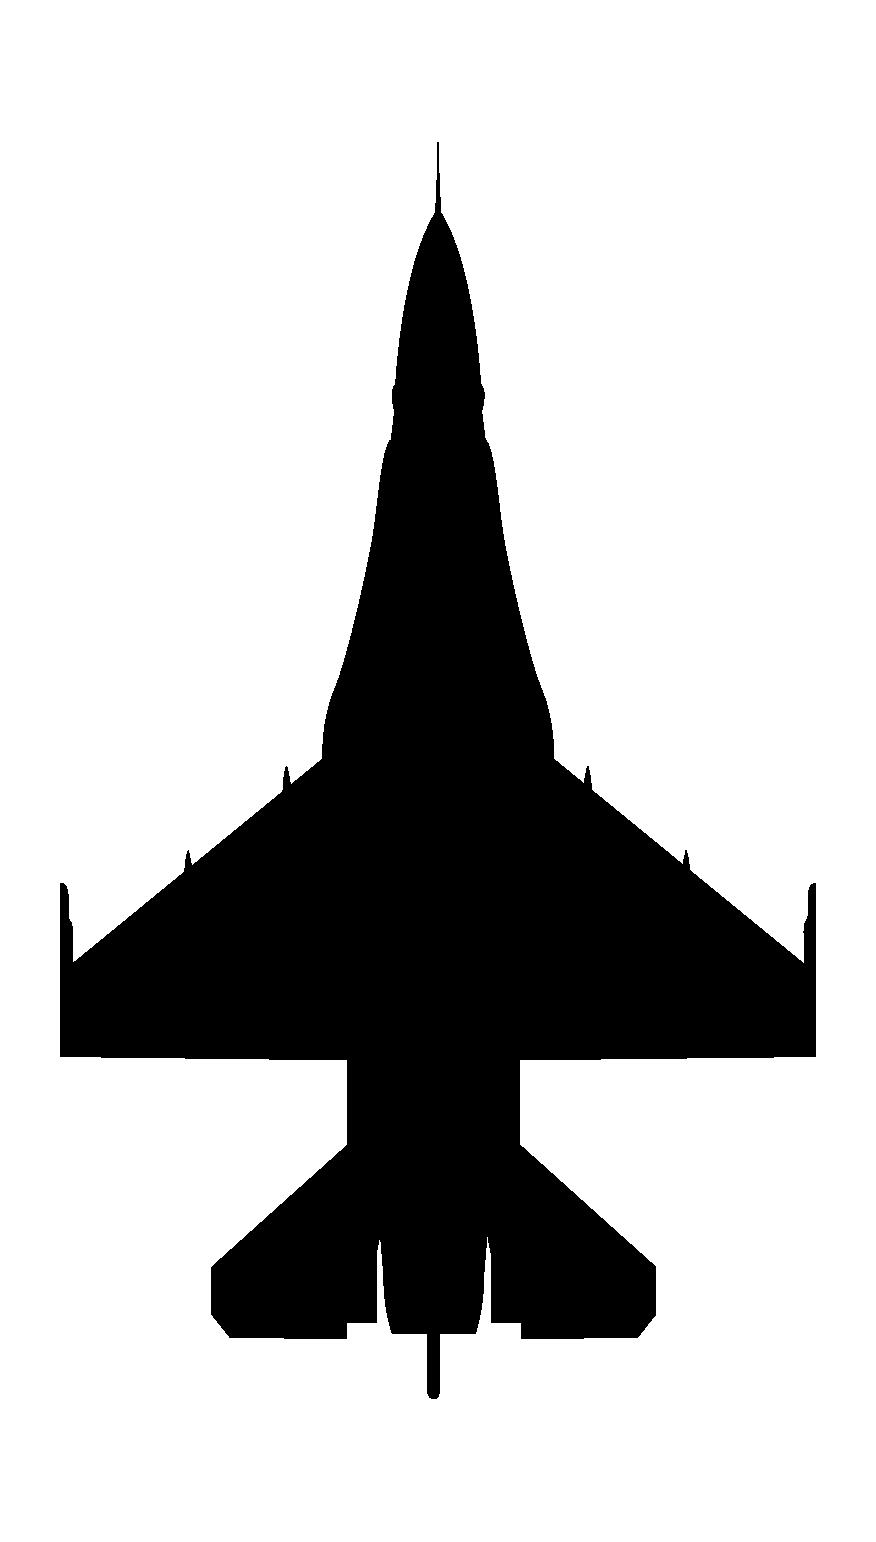
\includegraphics[
                    width=7.5mm,
                ]{diagrams/aircraft/silhouette_f16_top.pdf}
            };
            \draw[->] 
            (0,0) -- 
            (0,5) arc (180:0:5) --
            (10,0) 
            node[rotate=-180, anchor=south, yshift=-1mm]{
                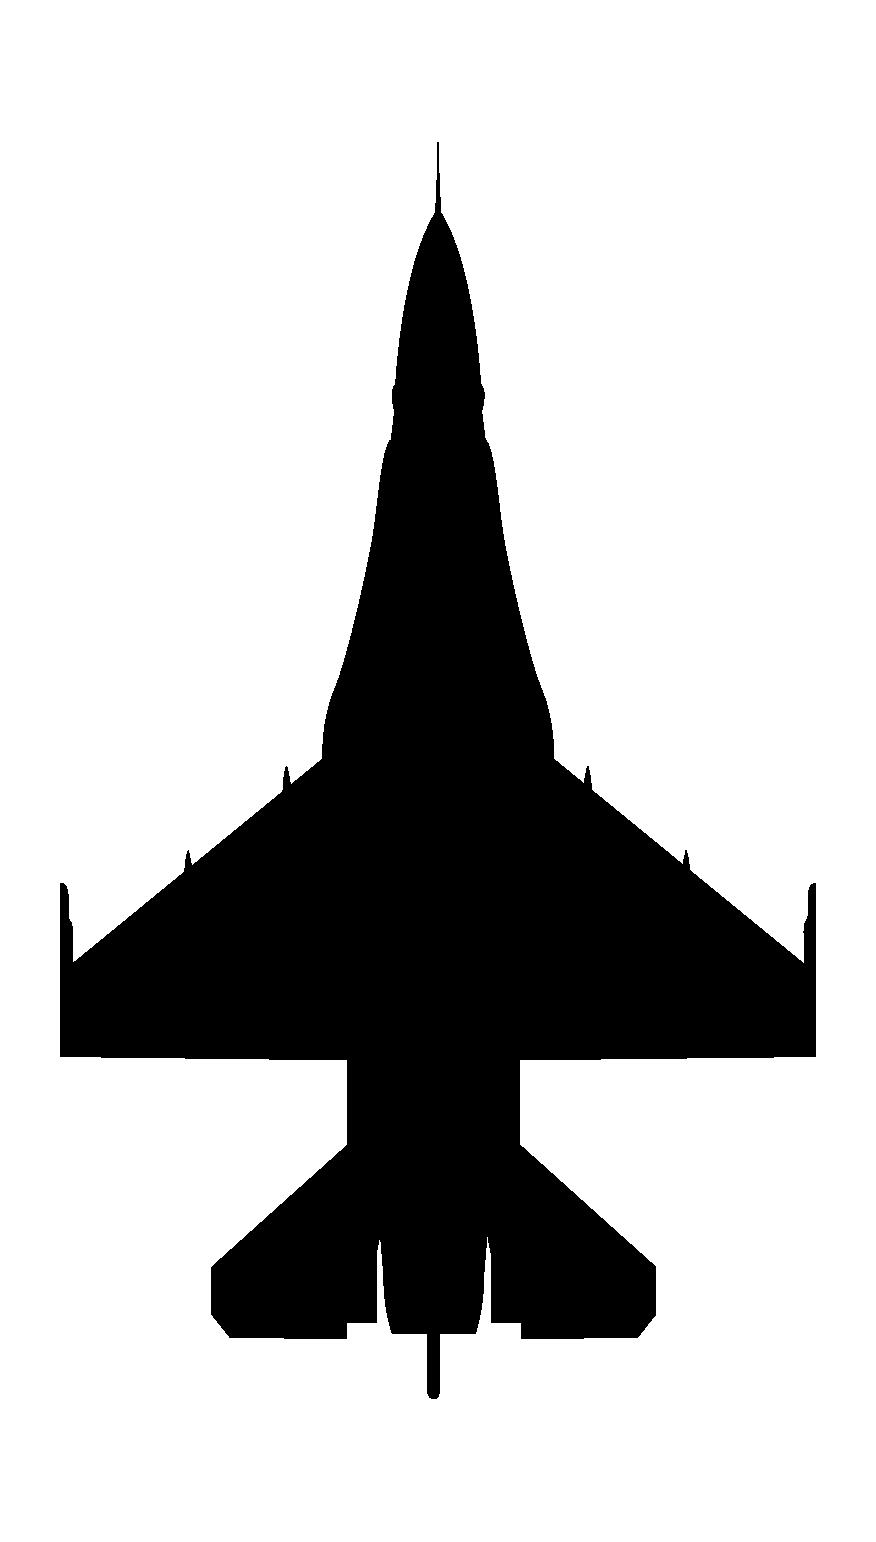
\includegraphics[
                width=7.5mm,
            ]{diagrams/aircraft/silhouette_f16_top.pdf}};
    
            % BANDIT
            \draw[rounded corners, ->] 
            (0,35) -- (0,25);

            % help line
            \draw[thin, dashed] 
            (0,25) -- (0,5);

        \end{tikzpicture}
        \caption{Go Cold}
        \label{fig:aa_weap:bvr:fightermaneuver:cold}
    \end{subfigure}
    \caption{Top-down view of basic BVR fighter maneuvers}
    \label{fig:aa_weap:bvr:fightermaneuver}
\end{figure}

\notebox{
    \textbf{Turning in after going cold can place fighter within bandit launch envelope}
}

\subsubsection{TARGET ASPECT}

\begin{tcoloritemize}
    \blueitem[Target Aspect]
    Angle between imaginary line connecting fighter-bandit and bandit heading
    \blueitem[Hot]
    \textbf{Target aspect --- 0-40 deg}
    \begin{itemize}
        \item offensive posture, maximizes closure
    \end{itemize}
    \blueitem[Flank]
    \textbf{Target aspect --- 40-70 deg}
    \begin{itemize}
        \item minimizes closure while maintaining radar track
    \end{itemize}
    \blueitem[Beam]
    \textbf{Target aspect --- 70-110 deg}
    \begin{itemize}
        \item defensive maneuver to break pulse-doppler radar track
    \end{itemize}
    \blueitem[Drag]
    \textbf{Target aspect --- 110-180 deg}
    \begin{itemize}
        \item defense to kinematically defeat missile
        \item often used in group tactics as ambush setup
    \end{itemize}
\end{tcoloritemize}

\begin{figure}[htbp]
    \centering
    \begin{subfigure}[b]{0.2\linewidth}
        \centering
        \begin{tikzpicture}[figstyle]
            % FIGHTER
            \node[
                anchor=north,
                yshift=1mm,
            ] (fighter) at (0,0) {
                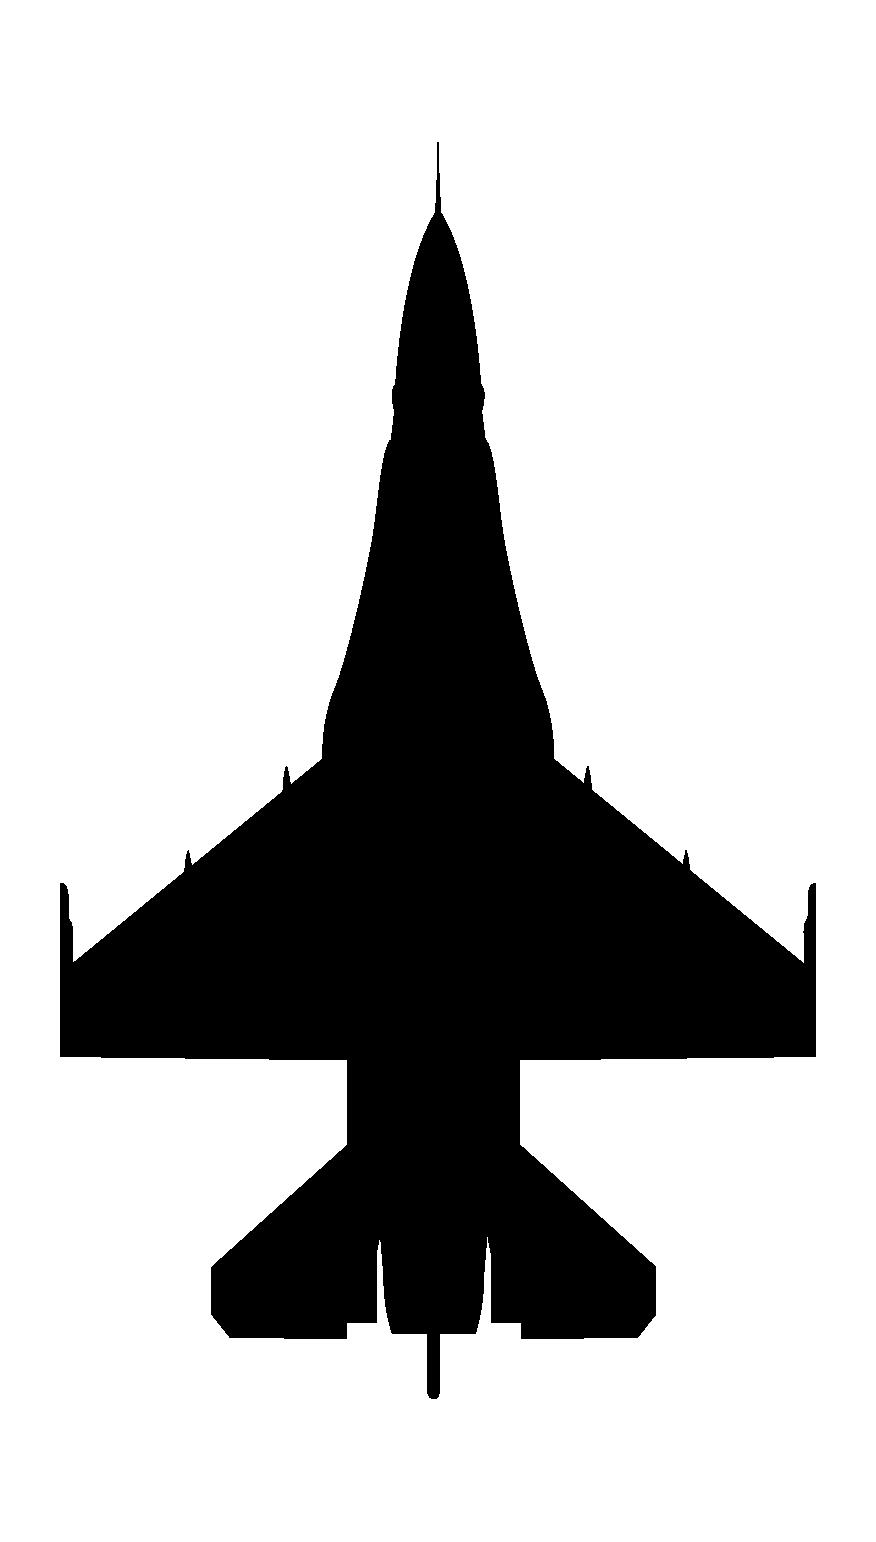
\includegraphics[
                    width=7.5mm,
                ]{diagrams/aircraft/silhouette_f16_top.pdf}
            };
    
            % BANDIT
            \draw[rounded corners, ->] 
            (0,20) -- +(-75:15);
    
            % help line
            \draw[thin, dashed] 
            (0,20) -- (0,0);
    
            \draw[thin]
            (0,10) arc (-90:-75:10) node[pos=1.0, right]{\small\titlefont 0-40$^\circ$};

        \end{tikzpicture}
        \caption{Hot}
        \label{fig:aa_weap:bvr:ta:hot}
    \end{subfigure}
    \begin{subfigure}[b]{0.2\linewidth}
        \centering
        \begin{tikzpicture}[figstyle]
            % FIGHTER
            \node[
                anchor=north,
                yshift=1mm,
            ] (fighter) at (0,0) {
                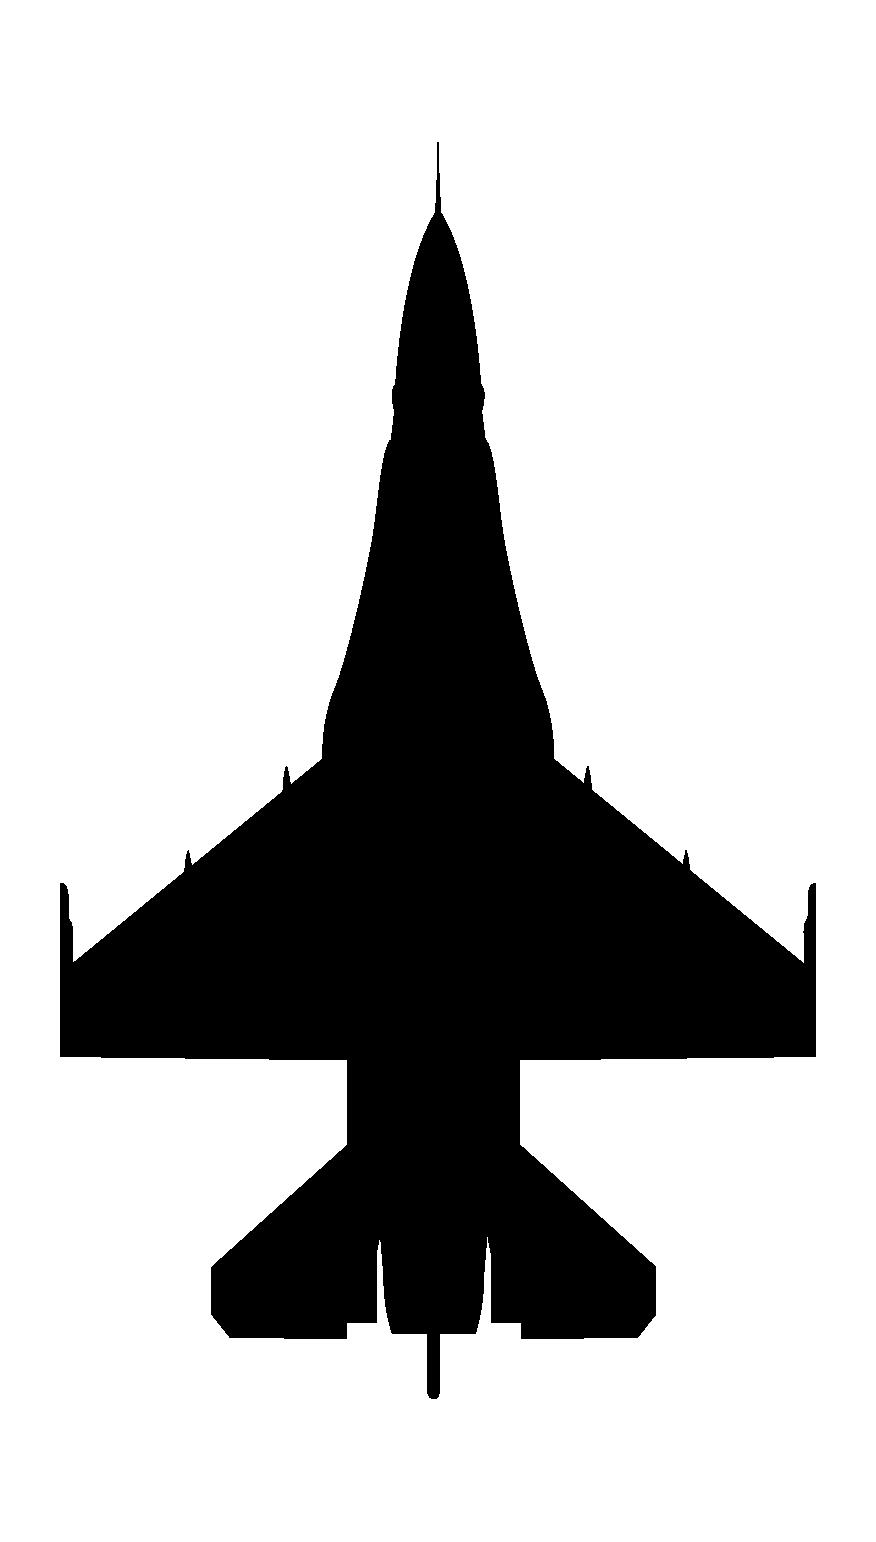
\includegraphics[
                    width=7.5mm,
                ]{diagrams/aircraft/silhouette_f16_top.pdf}
            };
    
            % BANDIT
            \draw[rounded corners, ->] 
            (0,20) -- +(-30:15);
    
            % help line
            \draw[thin, dashed] 
            (0,20) -- (0,0);
    
            \draw[thin]
            (0,10) arc (-90:-30:10) node[pos=0.25, below right]{\small\titlefont 40-70$^\circ$};

        \end{tikzpicture}
        \caption{Flank}
        \label{fig:aa_weap:bvr:ta:flank}
    \end{subfigure}
    \begin{subfigure}[b]{0.25\linewidth}
        \centering
        \begin{tikzpicture}[figstyle]
            % FIGHTER
            \node[
                anchor=north,
                yshift=1mm,
            ] (fighter) at (0,0) {
                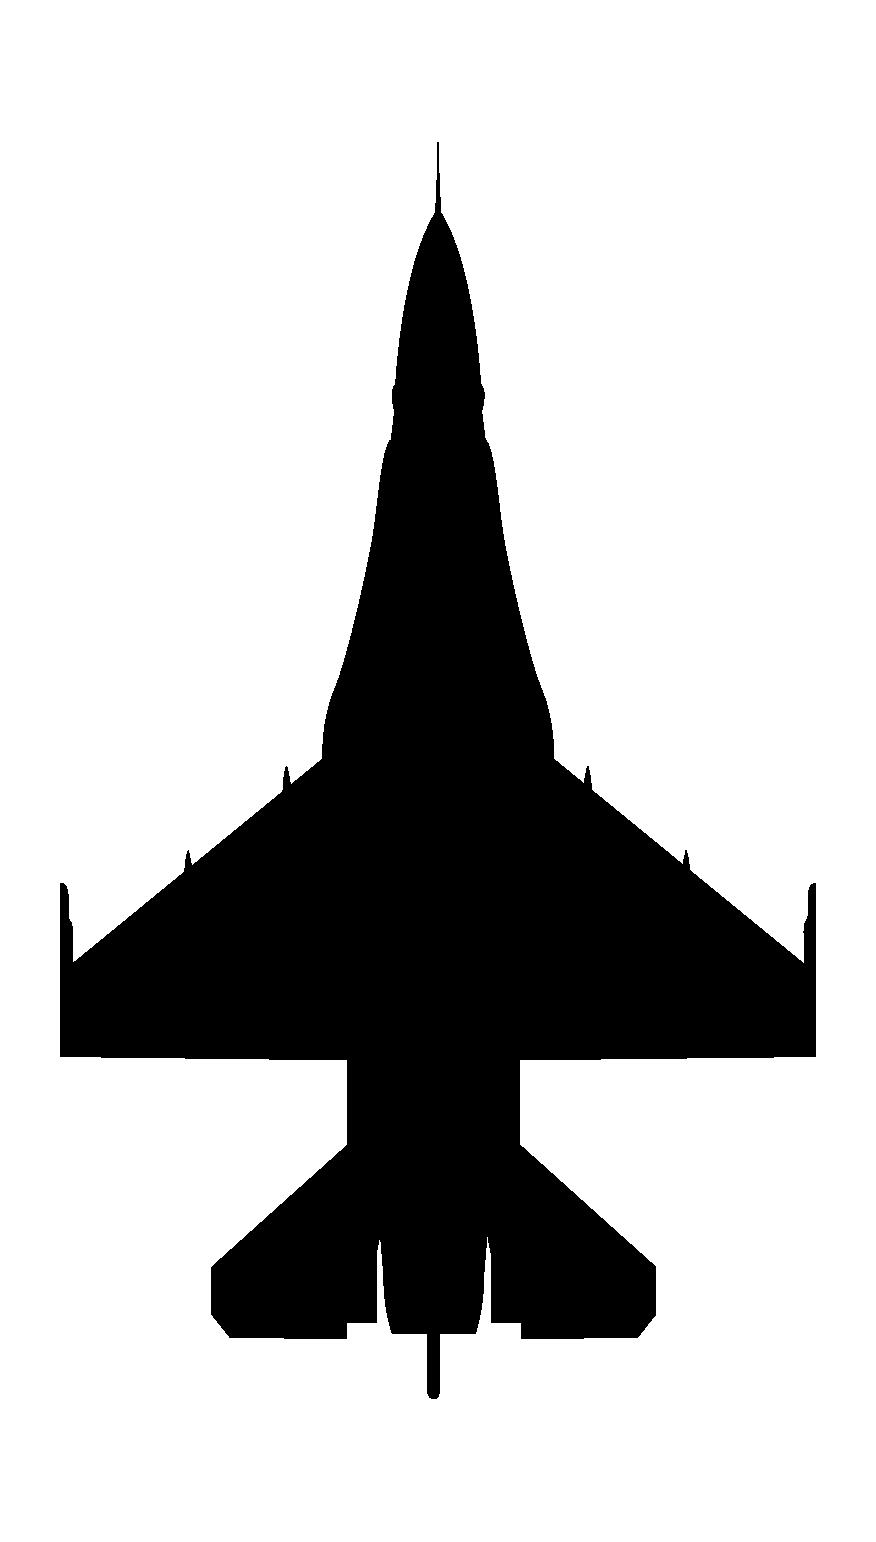
\includegraphics[
                    width=7.5mm,
                ]{diagrams/aircraft/silhouette_f16_top.pdf}
            };
    
            % BANDIT
            \draw[rounded corners, ->] 
            (0,20) -- +(0:15);
    
            % help line
            \draw[thin, dashed] 
            (0,20) -- (0,0);
    
            \draw[thin]
            (0,10) arc (-90:0:10) node[pos=0.25, below right]{\small\titlefont 70-110$^\circ$};
    
        \end{tikzpicture}
        \caption{Beam}
        \label{fig:aa_weap:bvr:ta:beam}
    \end{subfigure}
    \begin{subfigure}[b]{0.25\linewidth}
        \centering
        \begin{tikzpicture}[figstyle]
            % FIGHTER
            \node[
                anchor=north,
                yshift=1mm,
            ] (fighter) at (0,0) {
                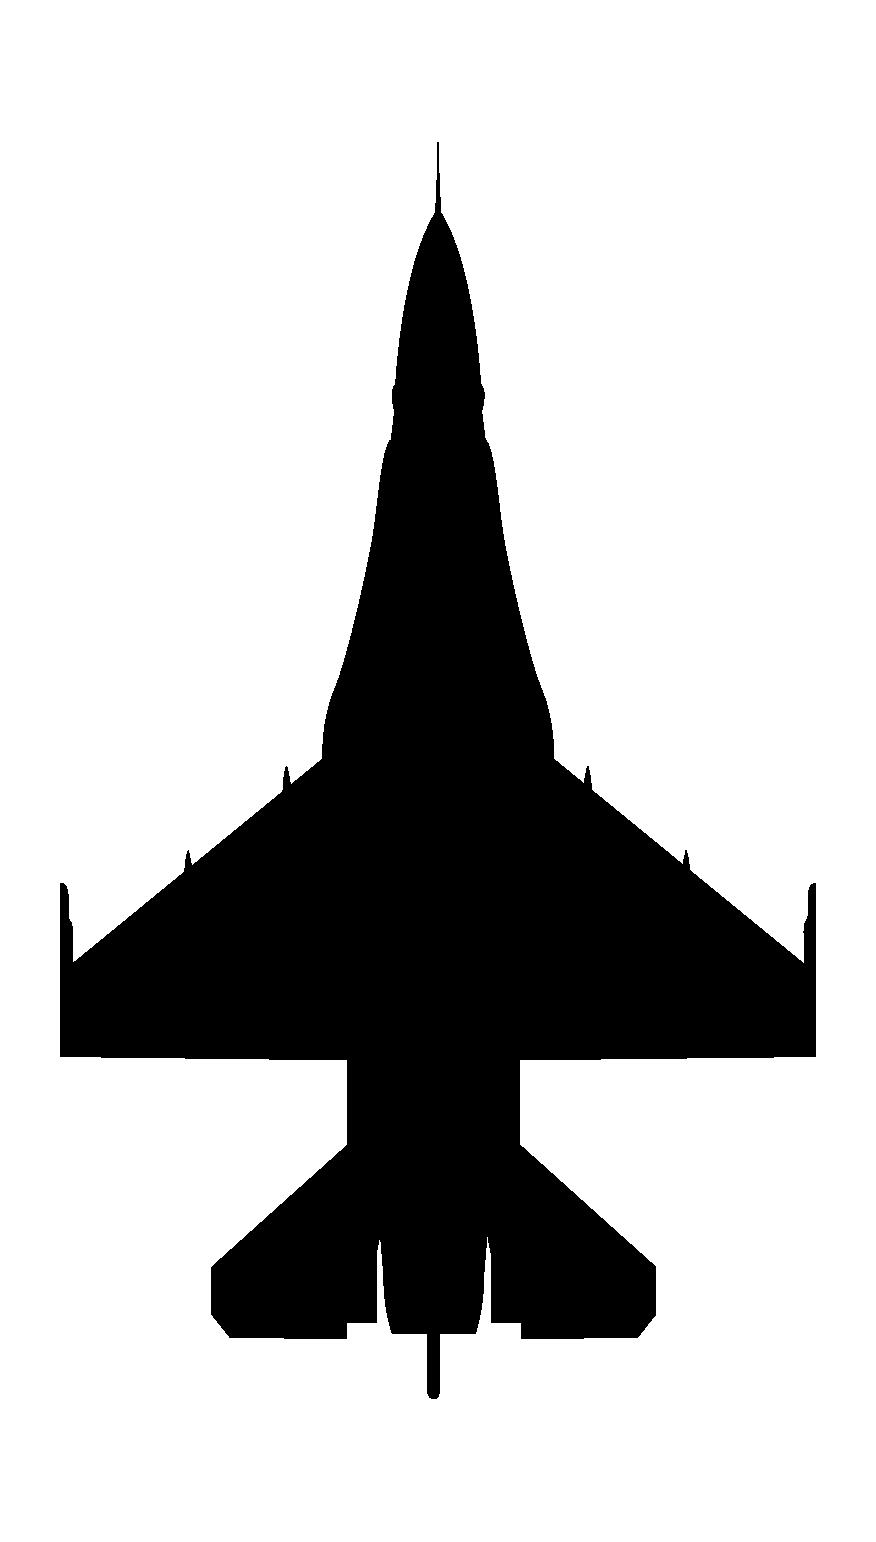
\includegraphics[
                    width=7.5mm,
                ]{diagrams/aircraft/silhouette_f16_top.pdf}
            };
    
            % BANDIT
            \draw[rounded corners, ->] 
            (0,20) -- +(90:15);
    
            % help line
            \draw[thin, dashed] 
            (0,20) -- (0,0);
    
            \draw[thin]
            (0,10) arc (-90:90:10) node[pos=0.125, below right]{\small\titlefont 110-180$^\circ$};
    
        \end{tikzpicture}
        \caption{Drag}
        \label{fig:aa_weap:bvr:ta:drag}
    \end{subfigure}
    \caption{Top down view illustrating target aspect classification}
    \label{fig:aa_weap:bvr:ta}
\end{figure}

\marginfigeometry

\subsection{INTERCEPT TIMELINES}

% \subsubsection{SKATE}
% \subsubsection{SHORT SKATE}
% \subsubsection{BANZAI}

\marginpar{
    \captionsetup{type=figure}
    \centering
    \begin{tikzpicture}[figstyle]
        
        \draw[->] 
            (0,0) -- 
            node[below, pos=0]{
                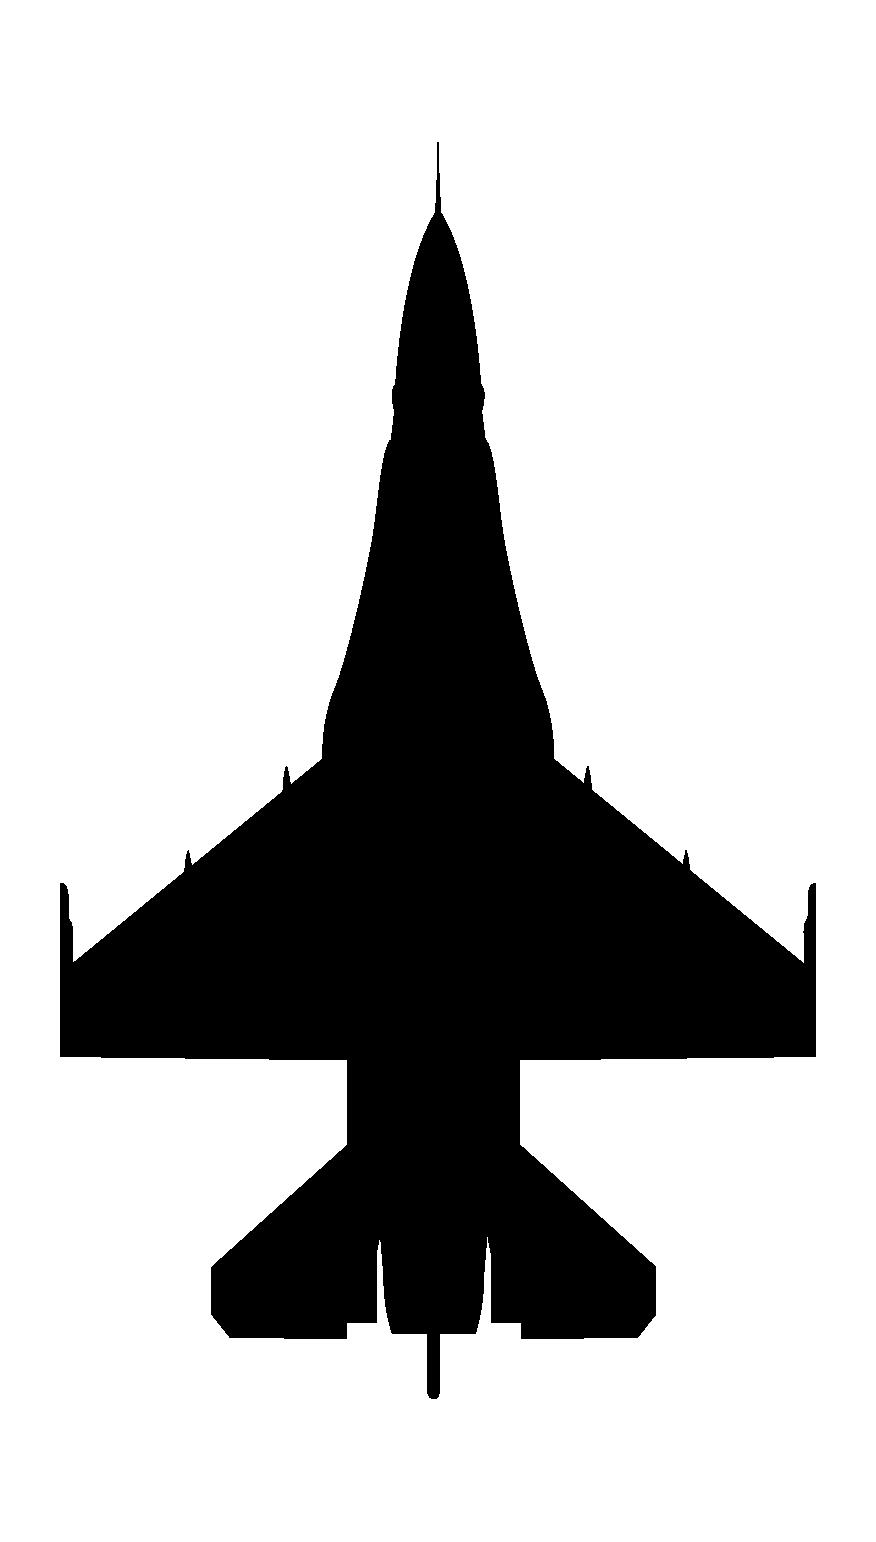
\includegraphics[
                width=7.5mm,
            ]{diagrams/aircraft/silhouette_f16_top.pdf}} 
            ++(0,20) 
            arc (180:90:5) 
            arc (-90:0:5) 
            -- ++(0,20) 
            arc (180:0:5) 
            -- ++(0,-50)
            node[below, pos=1, ]{
                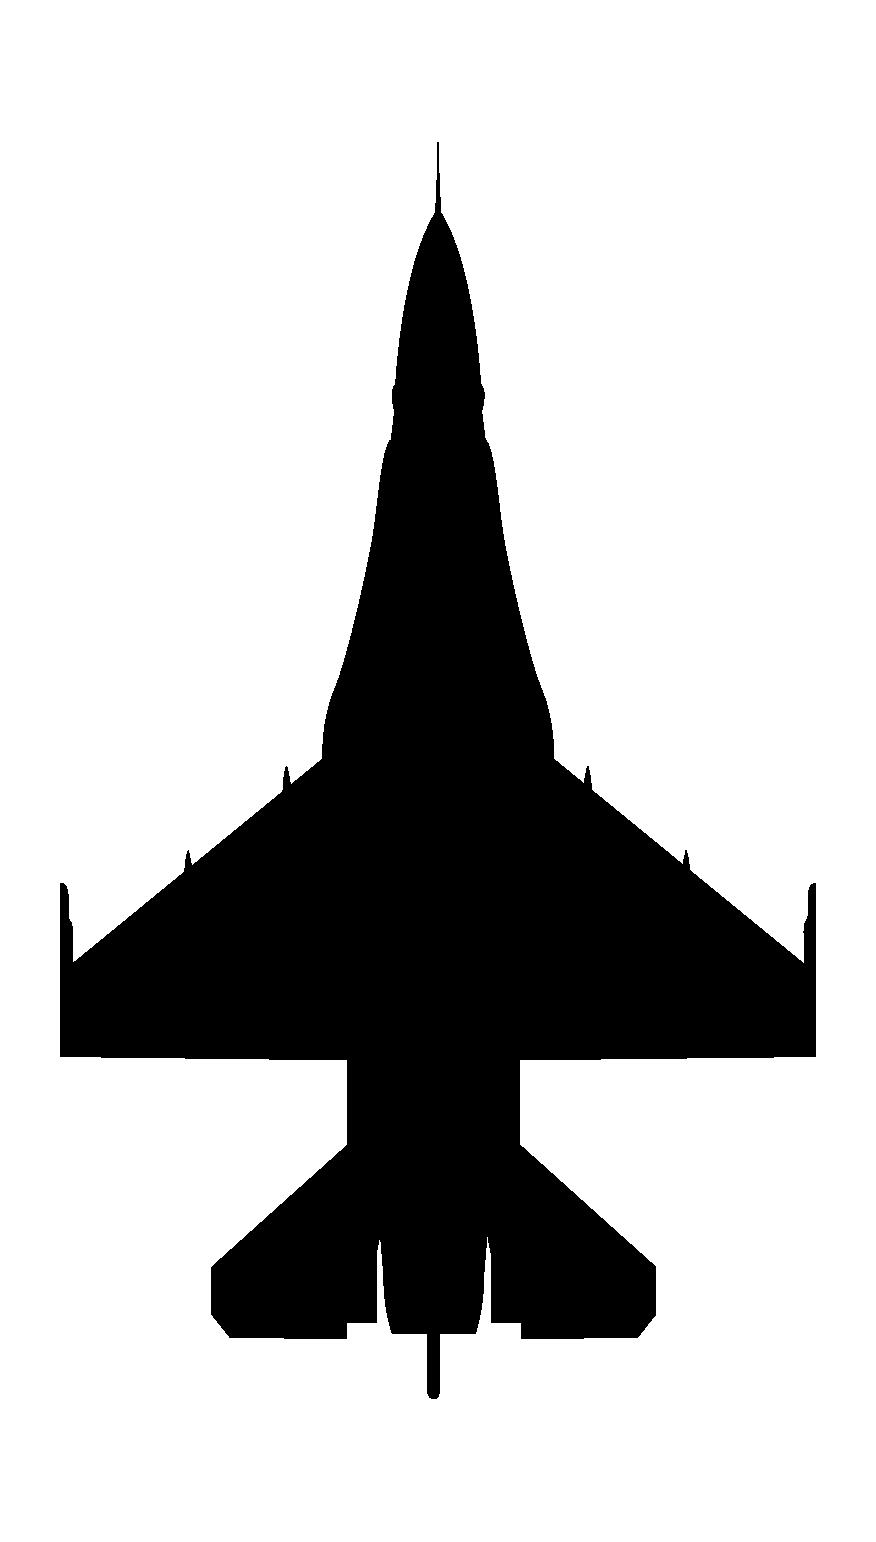
\includegraphics[
                    angle=180,
                    width=7.5mm,
            ]{diagrams/aircraft/silhouette_f16_top.pdf}};

    \end{tikzpicture}
    \caption{Work in progress timeline illustration}
}
\begin{center}
    \vspace{\textheight/4}
    \Large\titlefont\textbf{COMING SOON}
\end{center}

\marginfigrestore

\subsection{TWO-SHIP FORMATIONS}

\begin{tcoloritemize}
    \blueitem[Fighting Wing]
    \textbf{Easiest for wingman} --- used in low-threat areas

    \medskip

    \textbf{Advantages}
    \begin{itemize}
        \item easy to maintain
        \item leader's 6'o'clock covered
        \item allows heads-down time
    \end{itemize}

    \textbf{Disadvantages}
    \begin{itemize}
        \item wingman's 6'o'clock NOT covered
        \item close proximity
    \end{itemize}

    Reference \cref{fig:aa_weap:form:fightingwing} for illustration
    \blueitem[Wedge]
    \textbf{Similar to fighting wing} --- more spaced out
    
    \medskip

    \textbf{Advantages}
    \begin{itemize}
        \item easy to maintain
        \item leader's 6'o'clock covered
        \item free for aggressive maneuvering
    \end{itemize}

    \textbf{Disadvantages}
    \begin{itemize}
        \item wingman's 6'o'clock NOT covered
        \item lead changes difficult
    \end{itemize}

    Reference \cref{fig:aa_weap:form:wedge} for illustration
\end{tcoloritemize}

\begin{figure}[htbp]
    \centering
    \begin{minipage}[b]{0.5\textwidth}
        \centering
        \begin{tikzpicture}[figstyle]
            
            \coordinate (lead) at (0,0);
            \coordinate (wing) at ($(lead)+(-45:27.5)$);
    
            \draw[dashed]
            (lead) -- ++(-30:15) arc (-30:-60:15) -- (lead);
    
            \draw[fill=color2!15]
            ($(lead)+(-30:15)$) 
            -- ++(-30:25) node[font=\footnotesize, pos=1, right] {30$^\circ$}
            arc  (-30:-60:40) 
            node[font=\footnotesize, below, pos=0.5, rotate=45] {0.5nm}
            node[font=\footnotesize, pos=1, below right] {60$^\circ$}
            -- ++(120:25)
            arc (-60:-30:15)
            node[font=\footnotesize, below, pos=0.5, rotate=45] {0.1nm};
    
            \node[yshift=-3mm] (leadfig) at (lead) {
                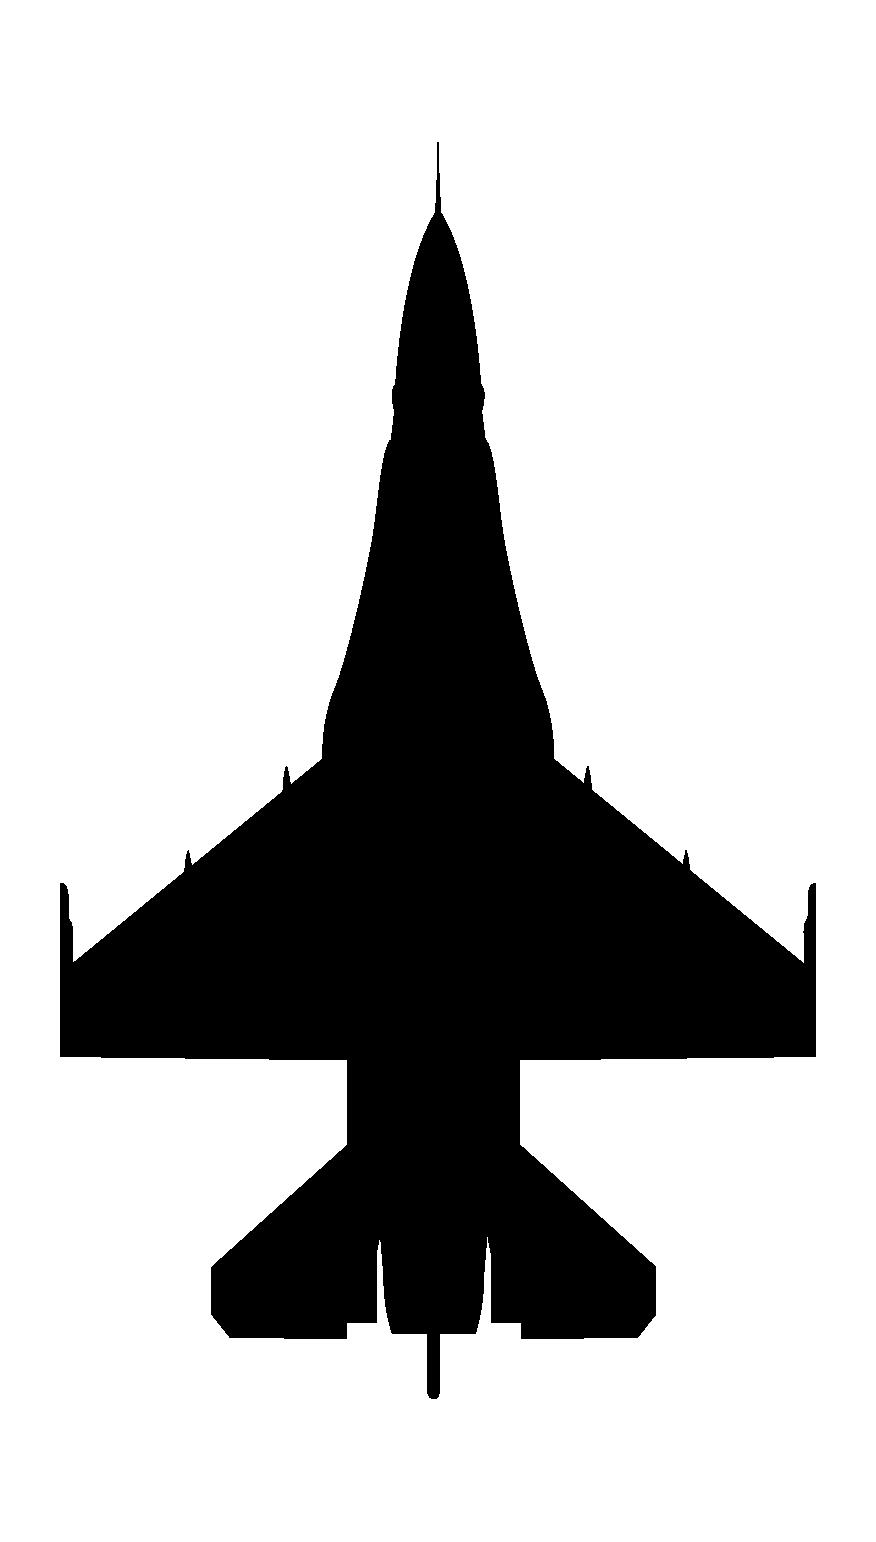
\includegraphics[
                    width=7.5mm,
                ]{diagrams/aircraft/silhouette_f16_top.pdf}
            };
            
            \node[] (wingfig) at (wing) {
                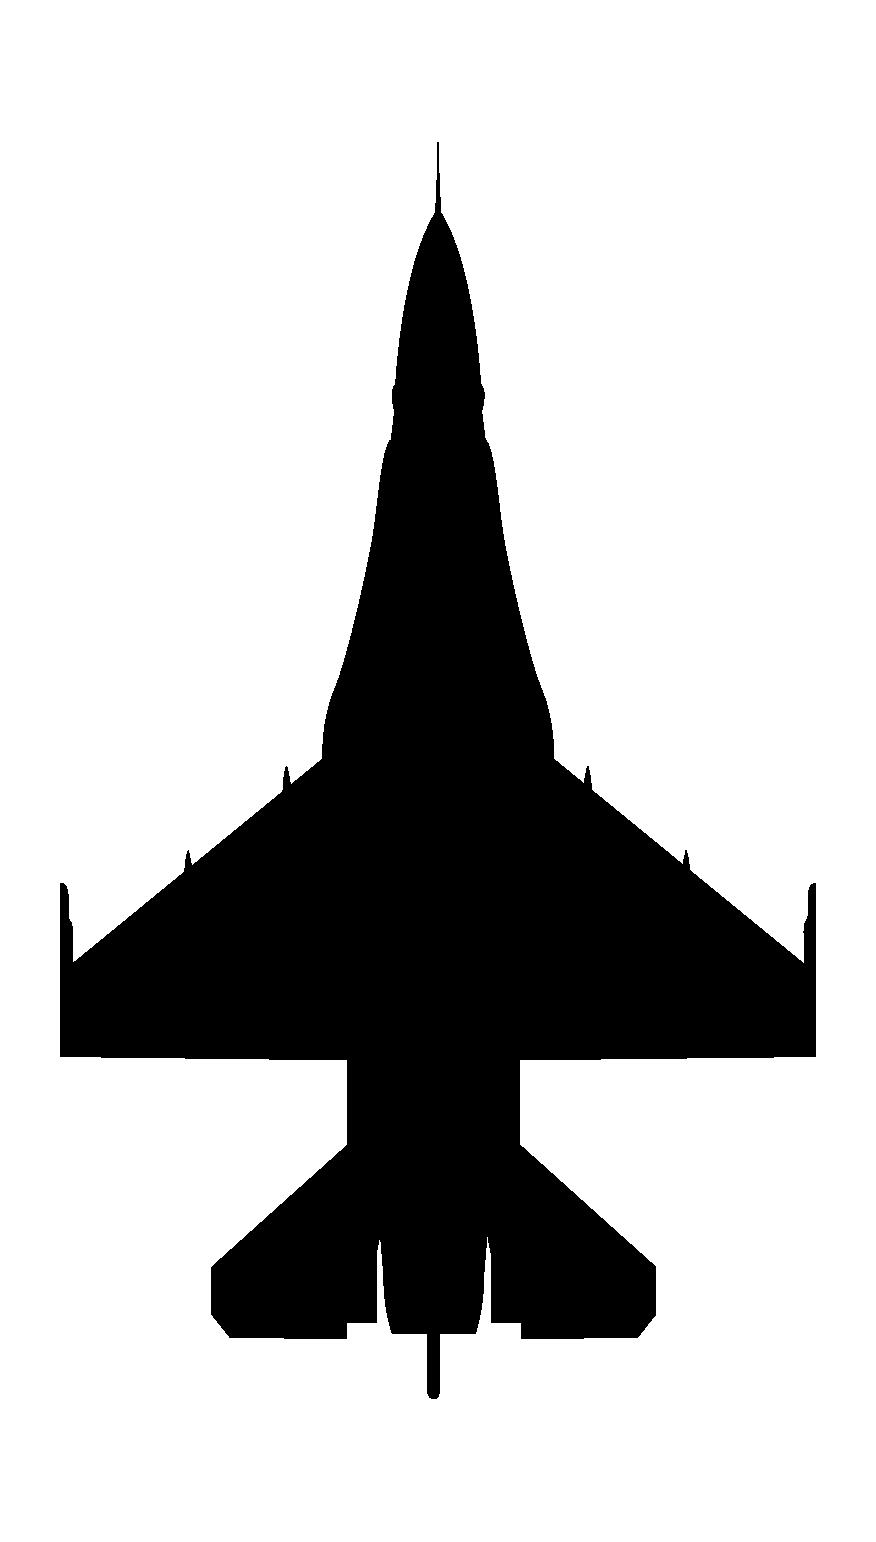
\includegraphics[
                    width=7.5mm,
                ]{diagrams/aircraft/silhouette_f16_top.pdf}
            };
    
        \end{tikzpicture}
        \caption{Fighting wing formation}
        \label{fig:aa_weap:form:fightingwing}
    \end{minipage}%
    \begin{minipage}[b]{0.5\textwidth}
        \centering
        \begin{tikzpicture}[figstyle]
            
            \coordinate (lead) at (0,0);
            \coordinate (wing) at ($(lead)+(-45:30)$);
    
            \draw[dashed]
            (lead) -- ++(-30:20) arc (-30:-60:20) -- (lead);
    
            \draw[fill=color2!15]
            ($(lead)+(-30:20)$) 
            -- ++(-30:20) node[font=\footnotesize, pos=1, right] {30$^\circ$}
            arc  (-30:-60:40) 
            node[font=\footnotesize, below, pos=0.5, rotate=45] {1.0 nm}
            node[font=\footnotesize, pos=1, below right] {60$^\circ$}
            -- ++(120:20)
            arc (-60:-30:20)
            node[font=\footnotesize, below, pos=0.5, rotate=45] {0.5 nm};
    
            \node[yshift=-3mm] (leadfig) at (lead) {
                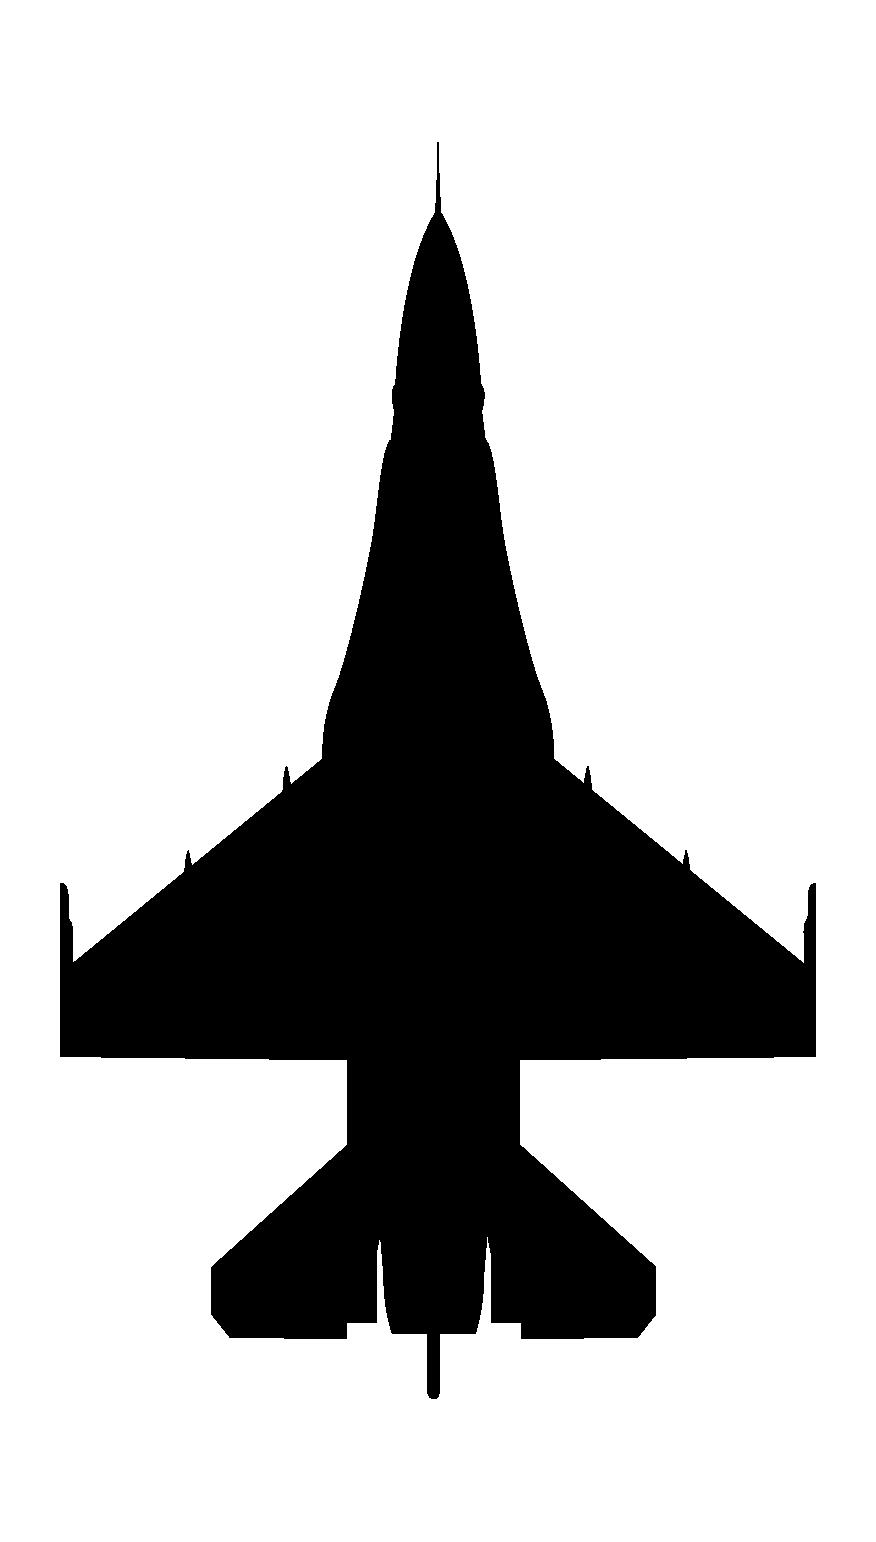
\includegraphics[
                    width=7.5mm,
                ]{diagrams/aircraft/silhouette_f16_top.pdf}
            };
            
            \node[] (wingfig) at (wing) {
                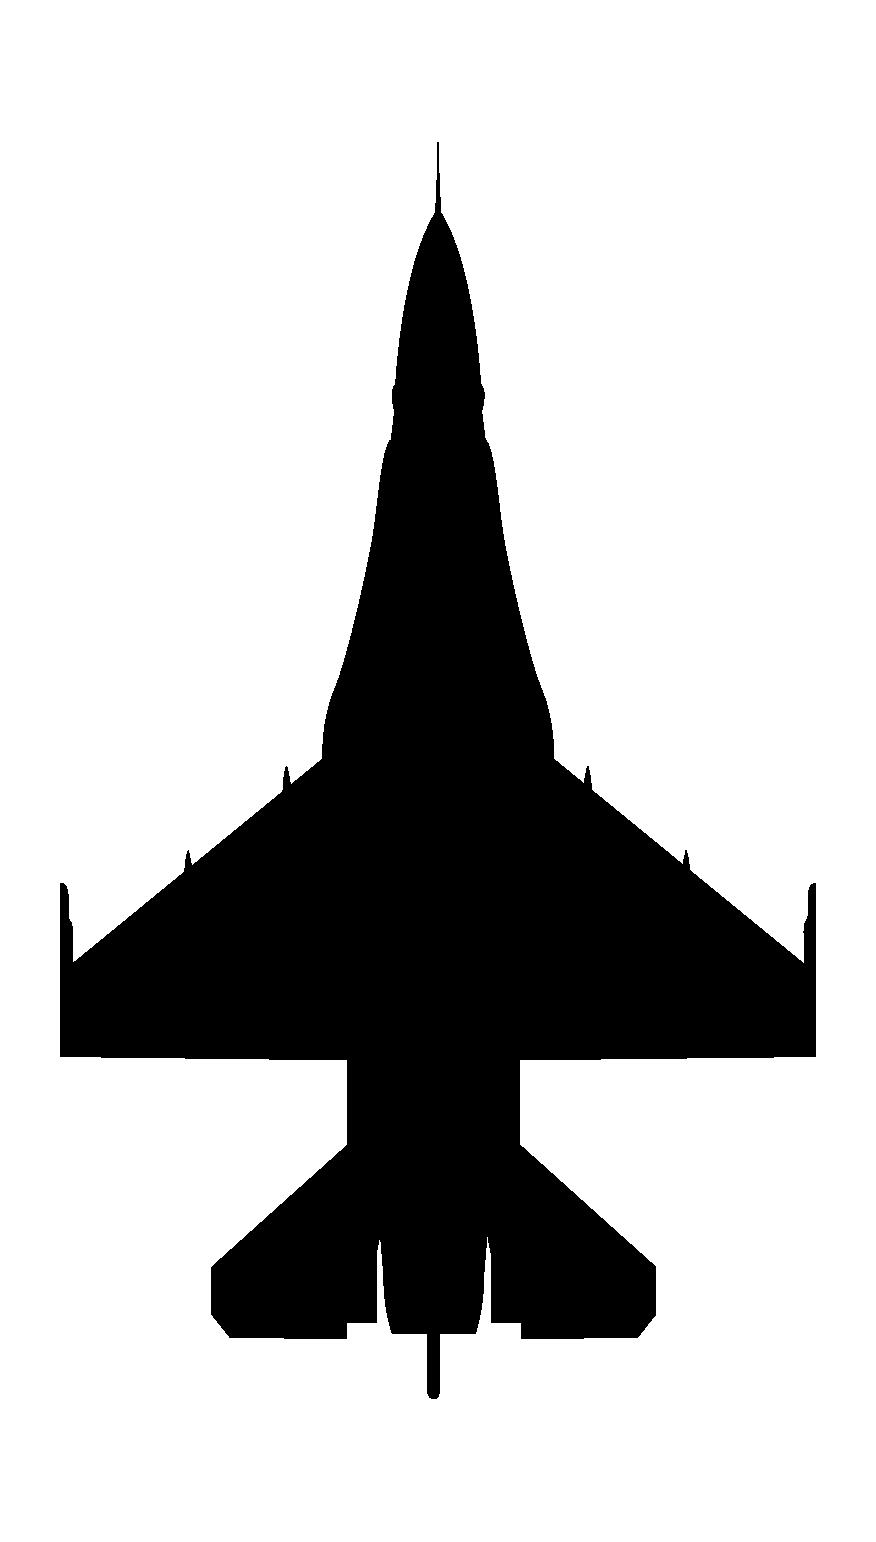
\includegraphics[
                    width=7.5mm,
                ]{diagrams/aircraft/silhouette_f16_top.pdf}
            };
    
        \end{tikzpicture}
        \caption{Two-ship wedge formation}
        \label{fig:aa_weap:form:wedge}
    \end{minipage}
\end{figure}

\begin{tcoloritemize}
    \blueitem[Line Abreast]
    \textbf{Tactical A-A Formation} --- mutual 6'o'clock cover, ensures all flight members in position to shoot simultaneously
    \medskip

    \textbf{Advantages}
    \begin{itemize}
        \item mutual 6'o'clock cover
        \item laterally spread
        \item simplifies tactical turns
        \item allows simultaneous bandit engagement
    \end{itemize}

    \textbf{Disadvantages}
    \begin{itemize}
        \item difficult to maintain
    \end{itemize}

    Reference \cref{fig:aa_weap:form:lineabreast} for illustration
\end{tcoloritemize}

\begin{figure}[htbp]
    \centering
    \begin{tikzpicture}[figstyle]
        
        \coordinate (lead) at (0,0);
        \coordinate (wing) at ($(lead)+(0:40)$);

        \draw[dashed]
        (lead) -- ++(0:20) arc (0:-20:20) -- (lead);

        \draw[fill=color2!15]
        ($(lead)+(0:20)$) 
        -- ++(0:40) node[font=\footnotesize, pos=1, right] {0$^\circ$}
        arc  (0:-20:60) 
        node[font=\footnotesize, right, pos=0.5] {2.0 nm}
        node[font=\footnotesize, pos=1, below right] {20$^\circ$}
        -- ++(160:40)
        arc (-20:0:20)
        node[font=\footnotesize, right, pos=0.5] {0.7 nm};

        \node[yshift=-3mm] (leadfig) at (lead) {
            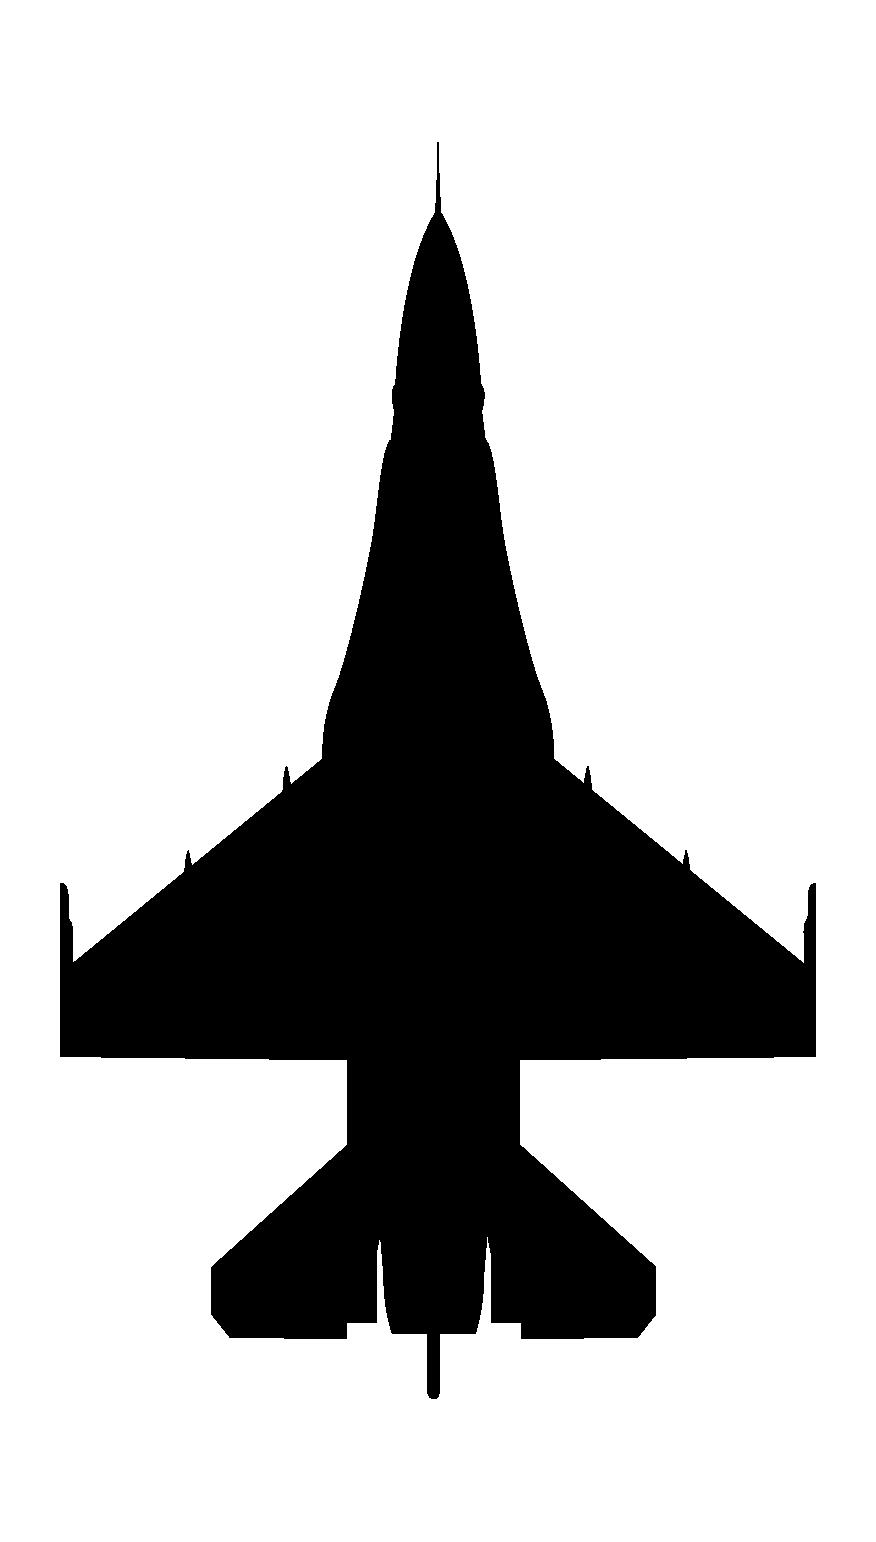
\includegraphics[
                width=7.5mm,
            ]{diagrams/aircraft/silhouette_f16_top.pdf}
        };
        
        \node[yshift=-3mm] (wingfig) at (wing) {
            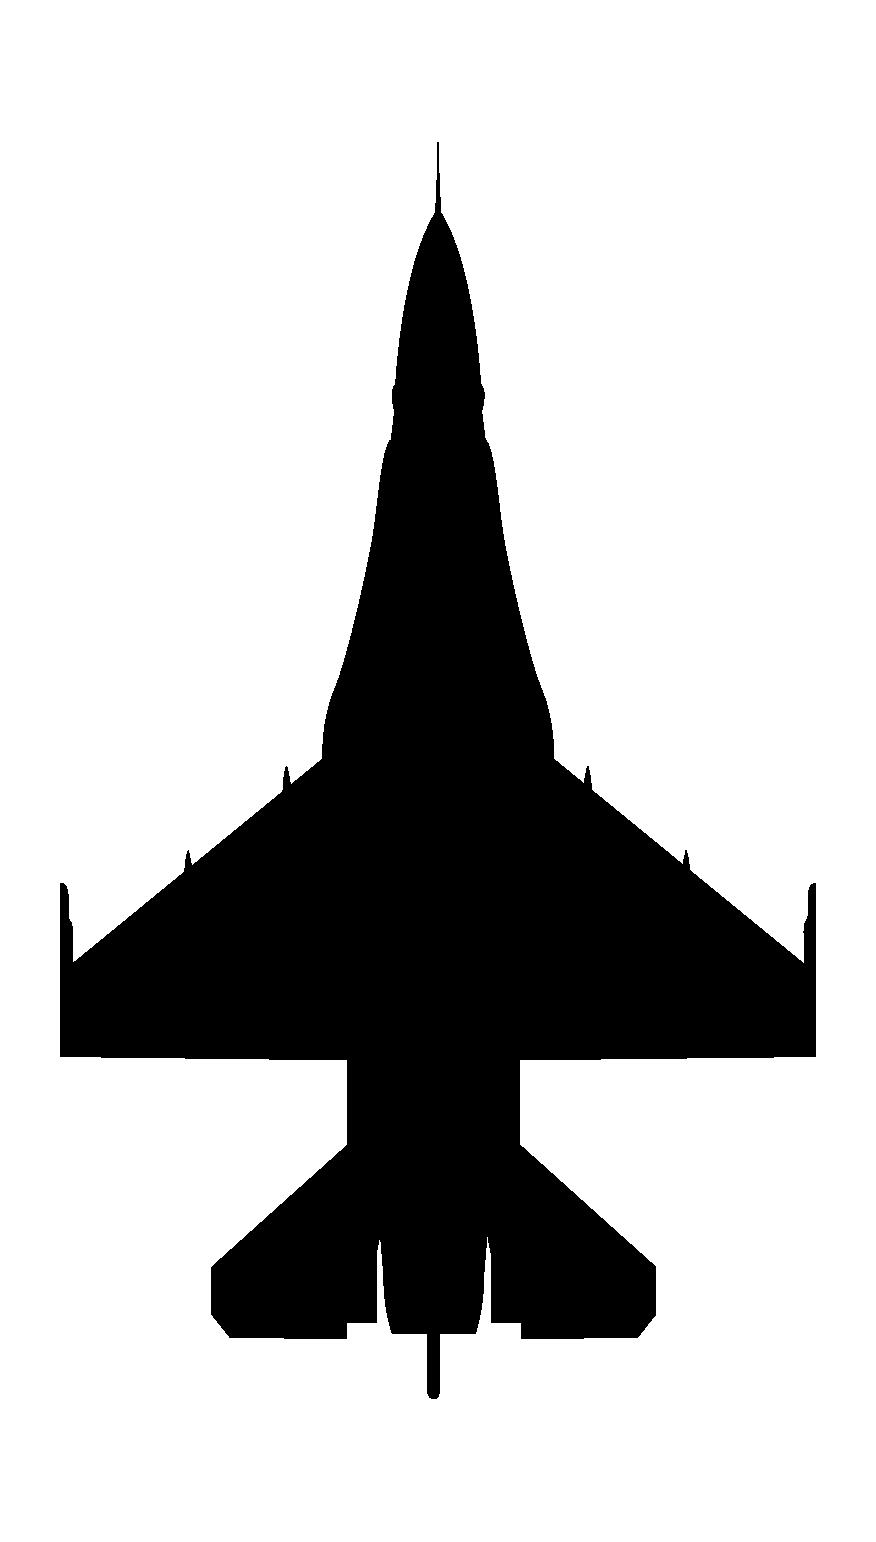
\includegraphics[
                width=7.5mm,
            ]{diagrams/aircraft/silhouette_f16_top.pdf}
        };

    \end{tikzpicture}
    \caption{Two-ship line abreast formation}
    \label{fig:aa_weap:form:lineabreast}
\end{figure}

\clearpage

\subsection{TACTICAL TURNS}

\begin{tcoloritemize}
    \blueitem[Tactical Turn]
    \textbf{Maintains line abreast formation}
    
    \begin{itemize}
        \item flight member on outside must initiate turn
    \end{itemize}
    \medskip

    Reference \cref{fig:aa_weap:form:tacturn} for illustration
\end{tcoloritemize}

\begin{figure}[htbp]
    \centering
    \begin{subfigure}[b]{0.45\linewidth}
        \centering
        \begin{tikzpicture}[figstyle]
            
            \draw[->] 
            (0,0) -- 
            node[below, pos=0]{
                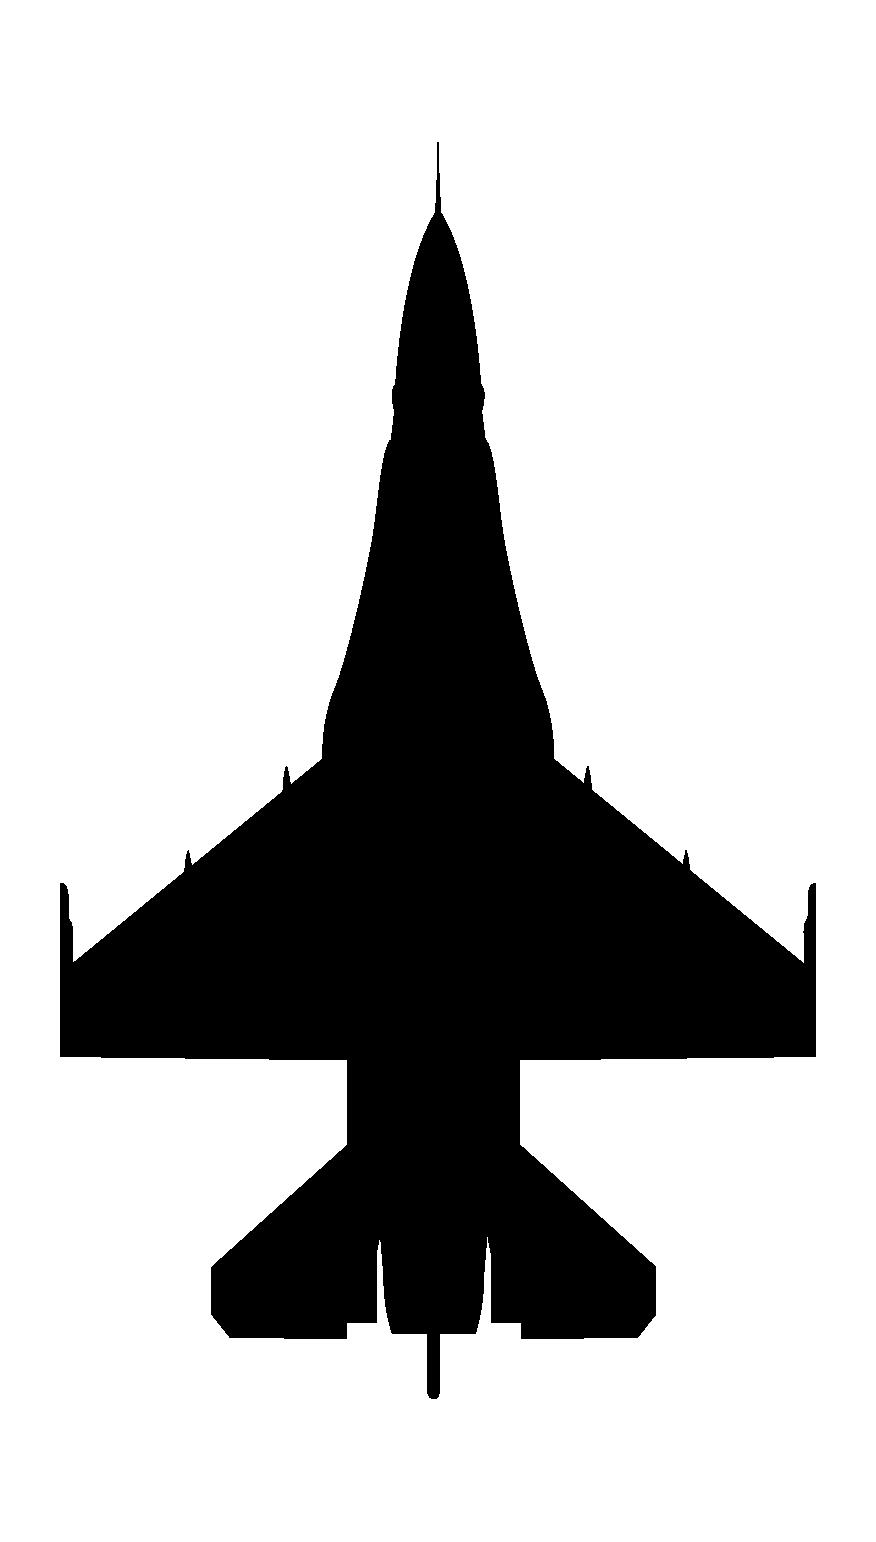
\includegraphics[
                width=7.5mm,
            ]{diagrams/aircraft/silhouette_f16_top.pdf}} 
            ++(0,10) 
            arc (180:90:10) 
            -- ++(20,0) 
            node[above, pos=1, rotate=-90]{
                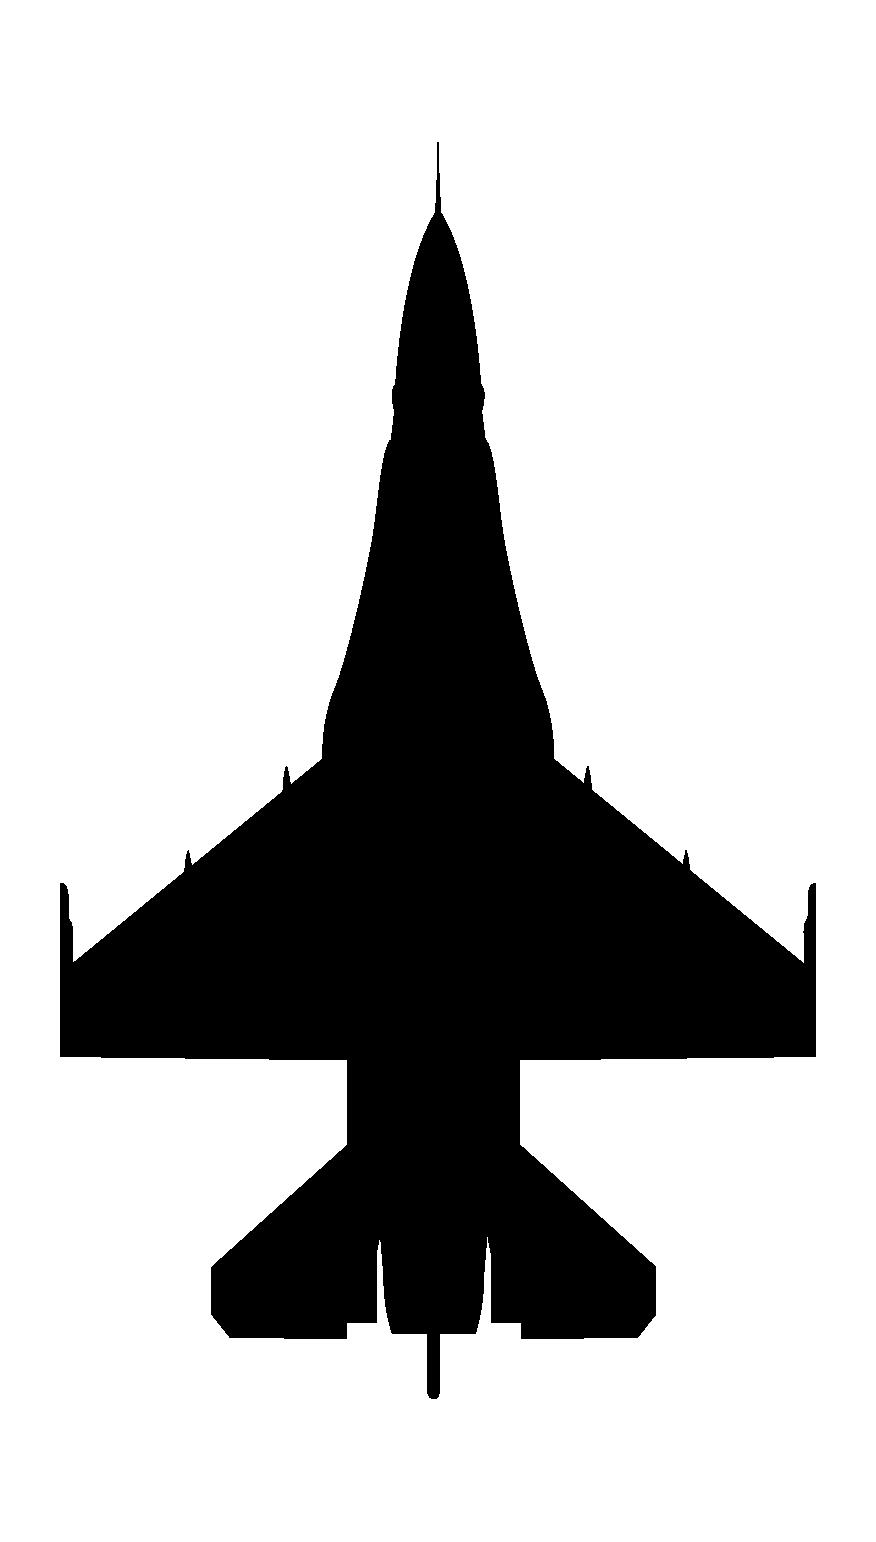
\includegraphics[
                    width=7.5mm,
            ]{diagrams/aircraft/silhouette_f16_top.pdf}};
                
            \draw[->] 
            (10,0) -- 
            node[below, pos=0]{
                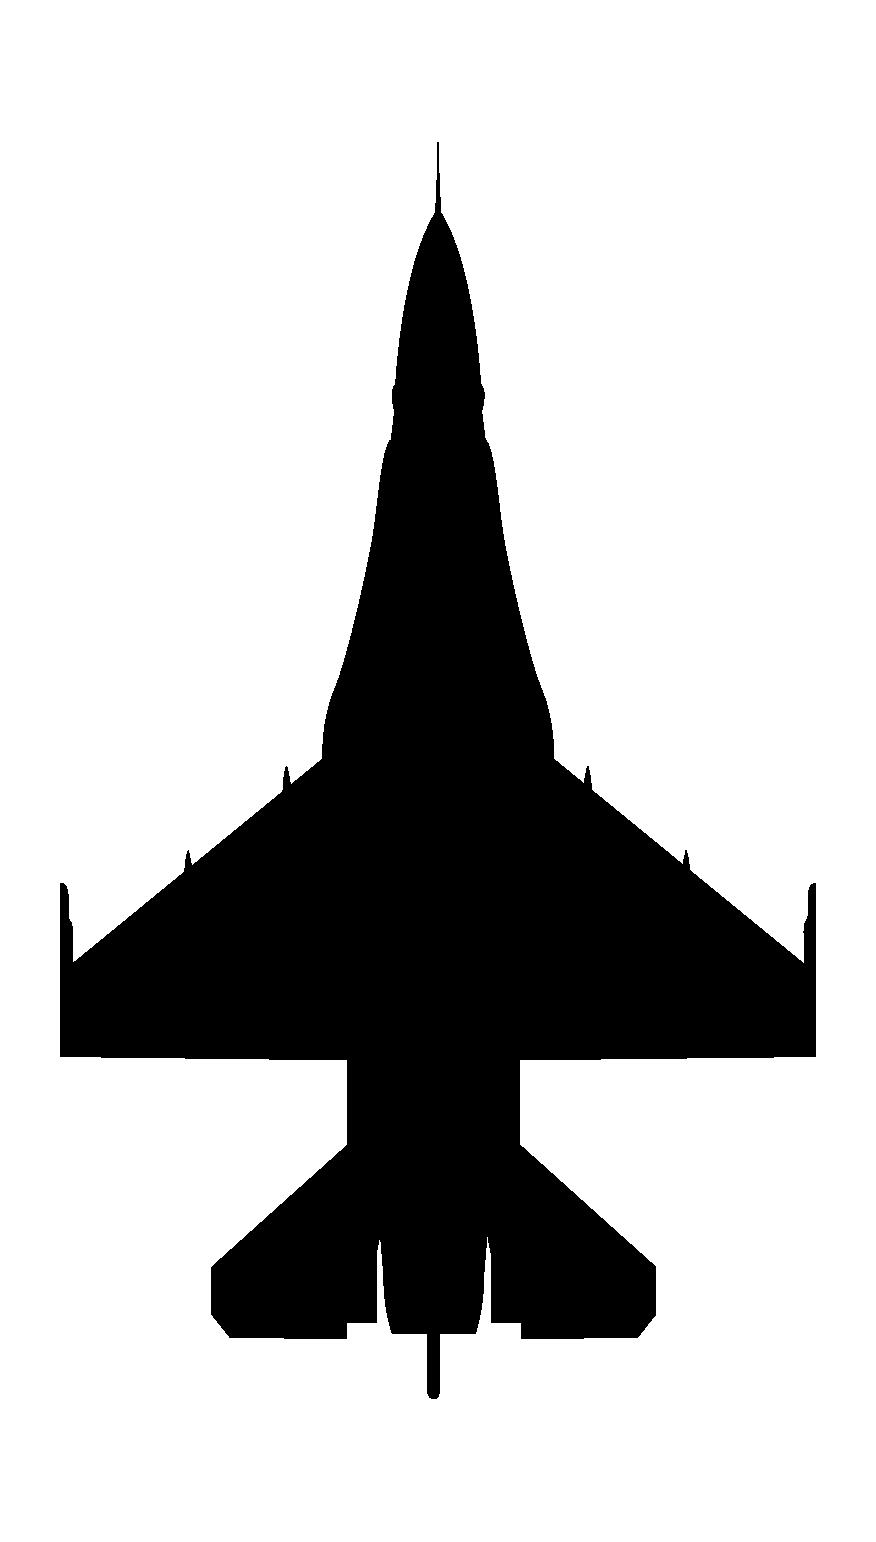
\includegraphics[
                width=7.5mm,
            ]{diagrams/aircraft/silhouette_f16_top.pdf}} 
            ++(0,20) 
            arc (180:90:10) 
            -- ++(10,0) 
            node[above, pos=1, rotate=-90]{
                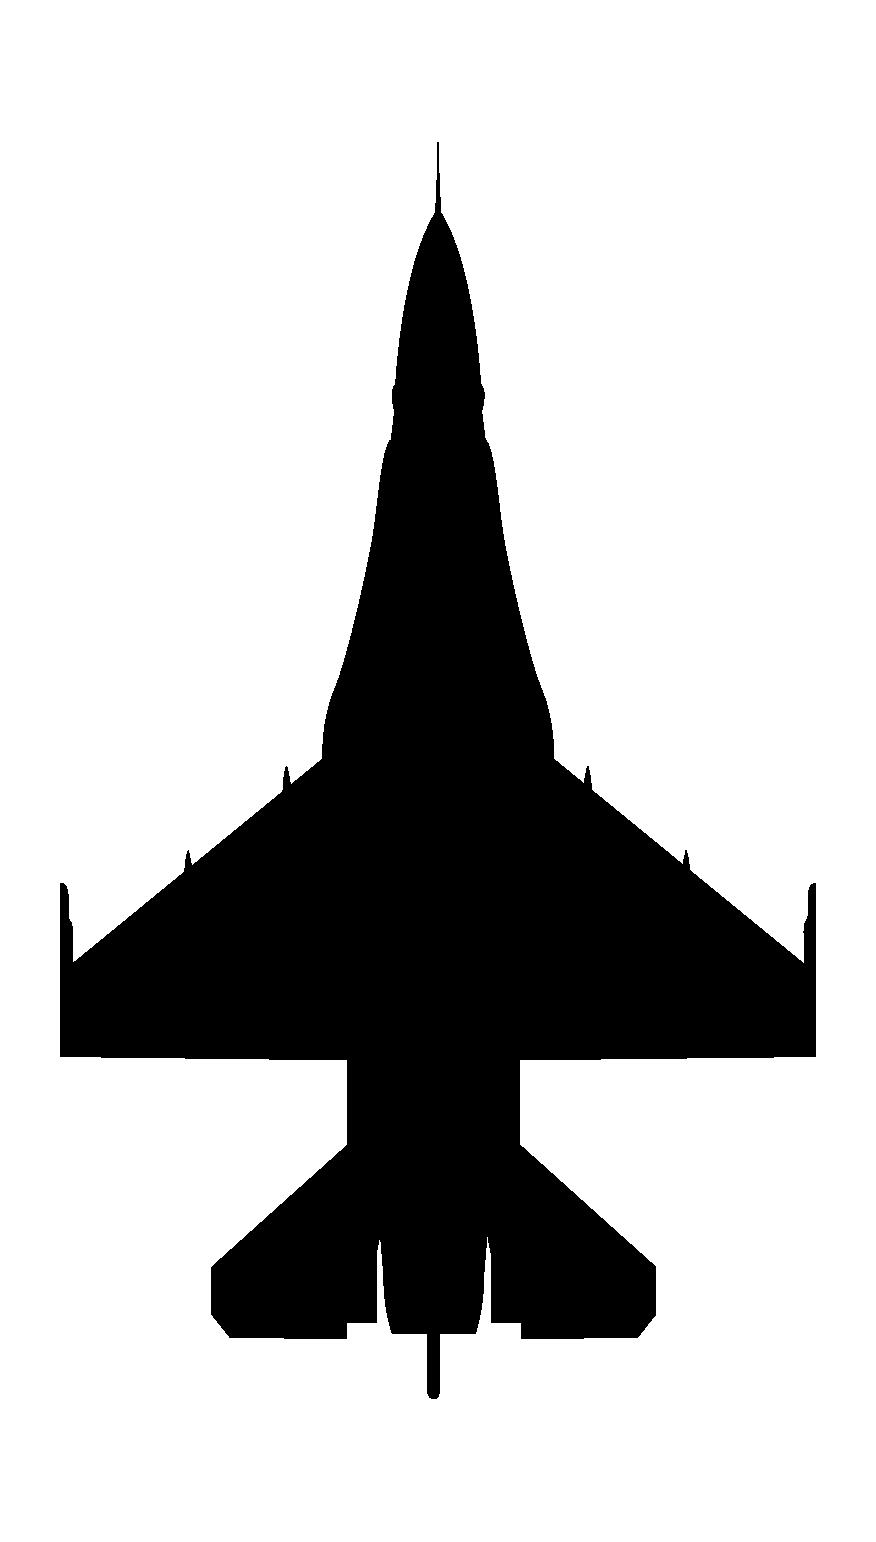
\includegraphics[
                    width=7.5mm,
            ]{diagrams/aircraft/silhouette_f16_top.pdf}};
        \end{tikzpicture}
        \caption{90 right}
    \end{subfigure}
    \begin{subfigure}[b]{0.45\linewidth}
        \centering
        \begin{tikzpicture}[figstyle]
            
            \draw[->] 
            (0,0) -- 
            node[below, pos=0]{
                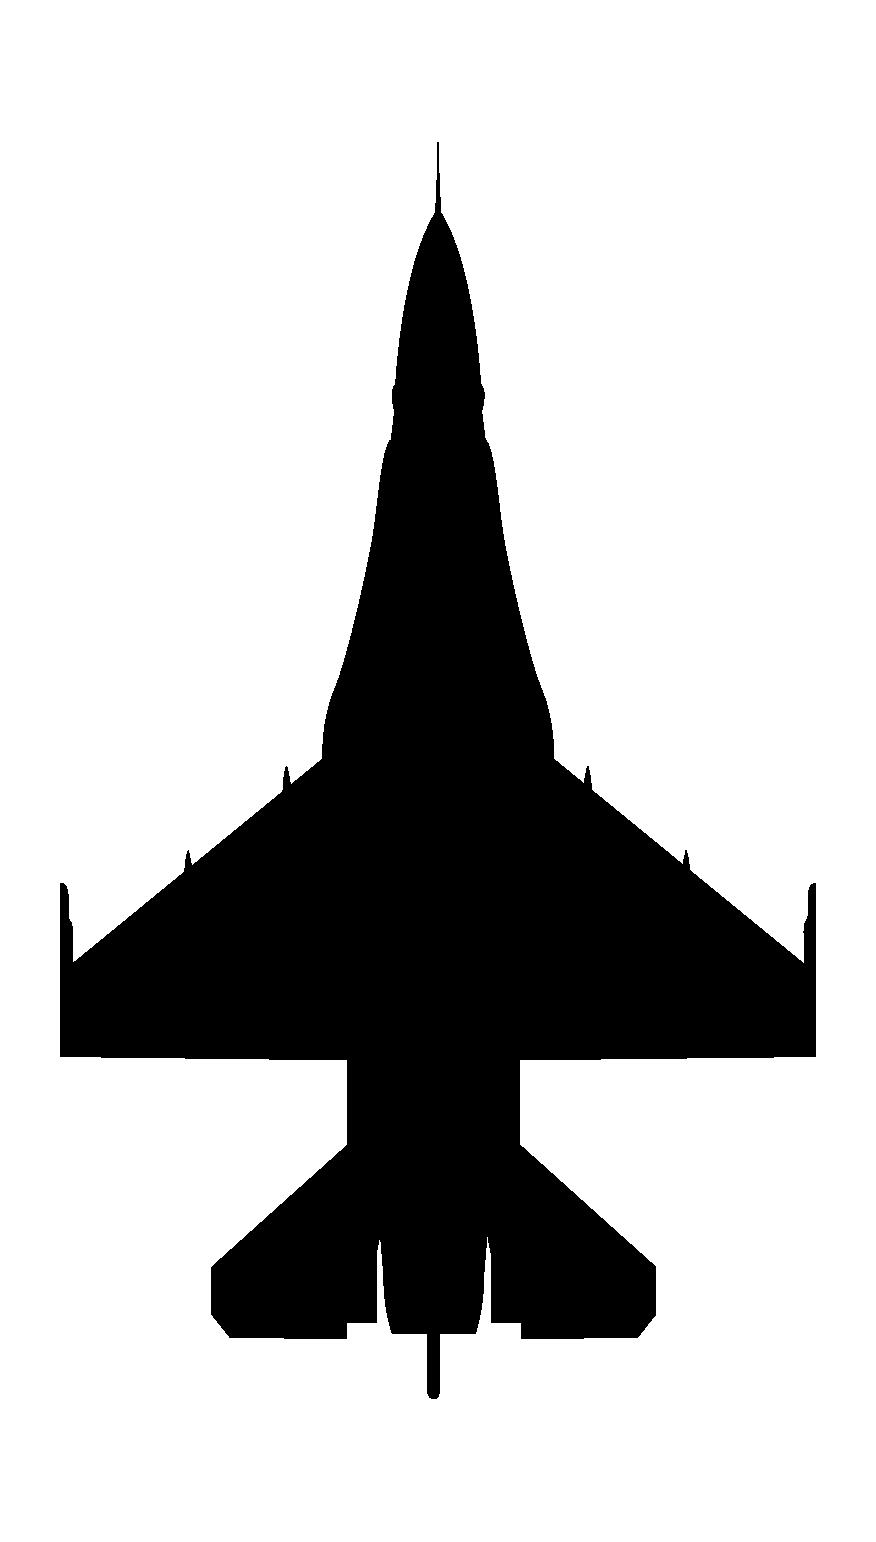
\includegraphics[
                width=7.5mm,
            ]{diagrams/aircraft/silhouette_f16_top.pdf}} 
            ++(0,27.5) 
            arc (0:45:10)  
            -- ++(-5,5) 
            node[above, pos=1, rotate=45]{
                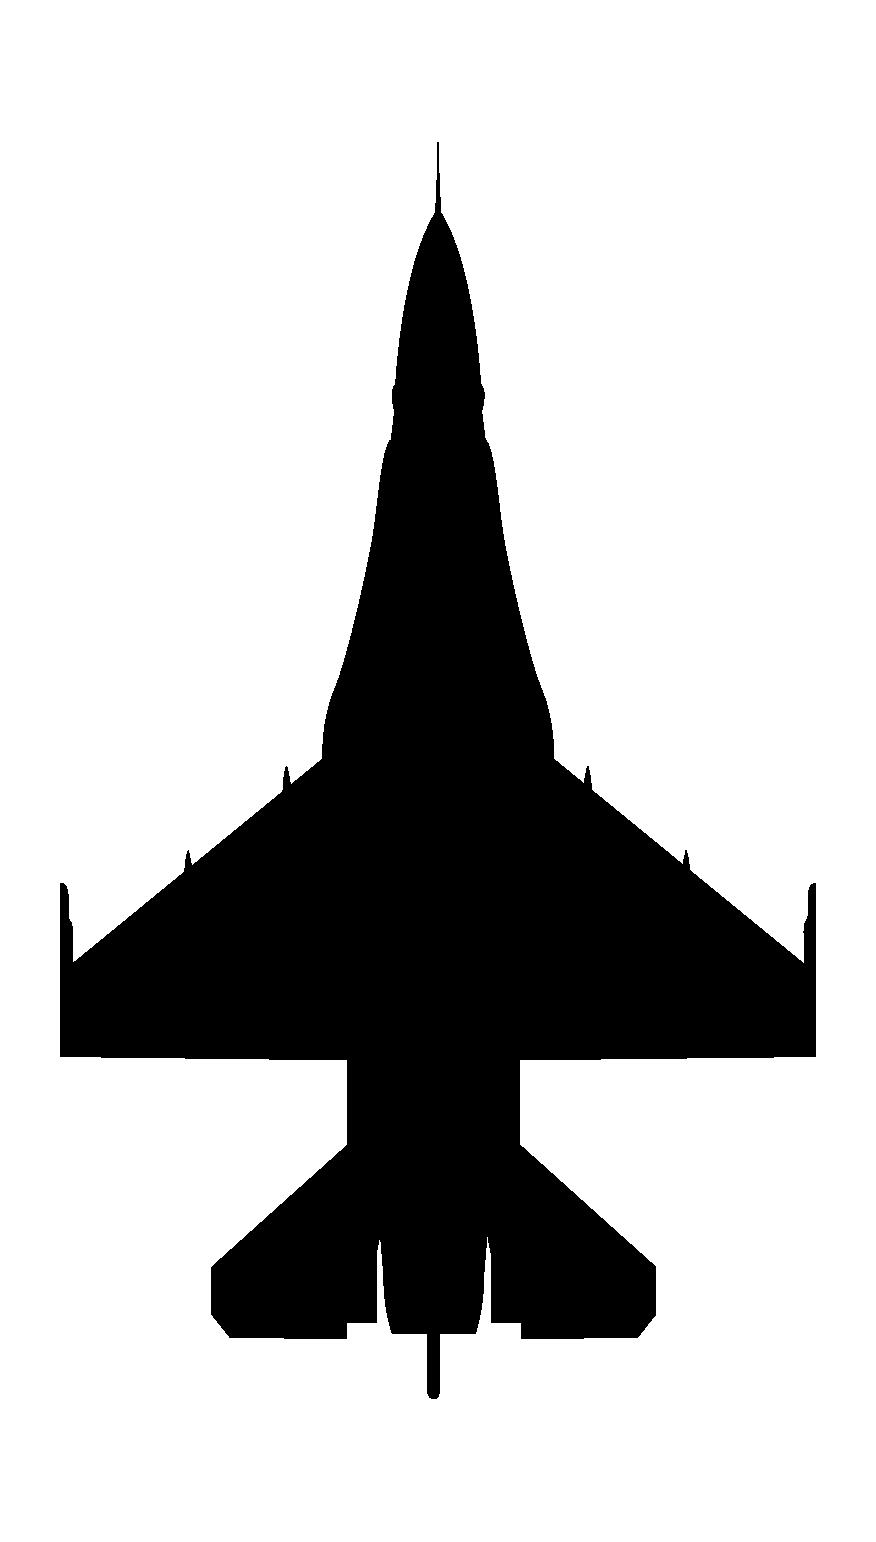
\includegraphics[
                    width=7.5mm,
            ]{diagrams/aircraft/silhouette_f16_top.pdf}};
                
            \draw[->] 
            (10,0) -- 
            node[below, pos=0]{
                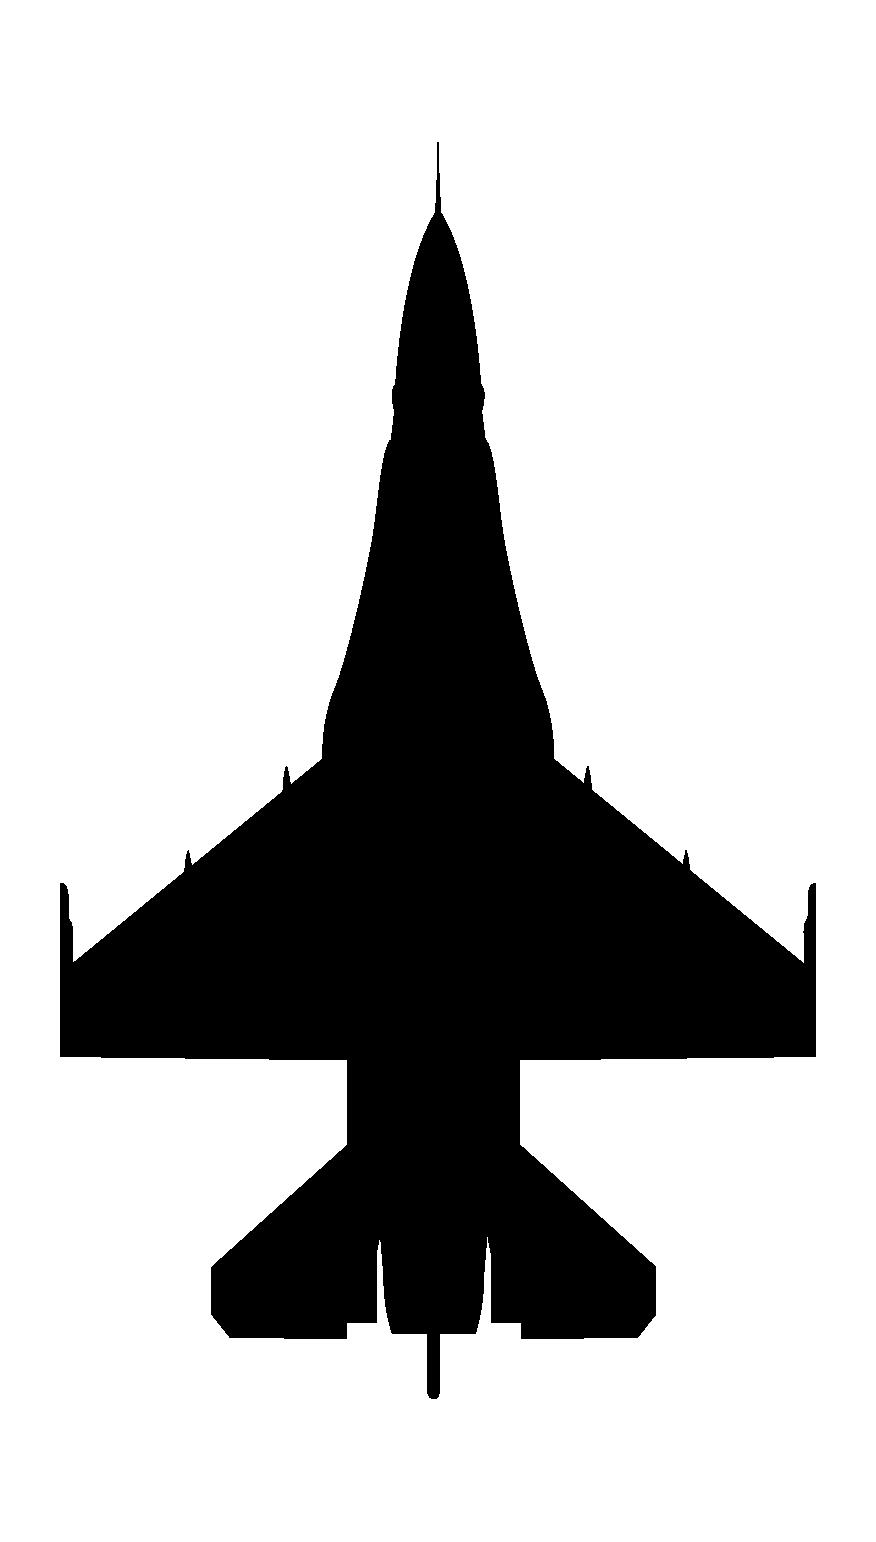
\includegraphics[
                width=7.5mm,
            ]{diagrams/aircraft/silhouette_f16_top.pdf}} 
            ++(0,2.5) 
            arc (0:45:10) 
            -- ++(-22.5,22.5) 
            node[above, pos=1, rotate=45]{
                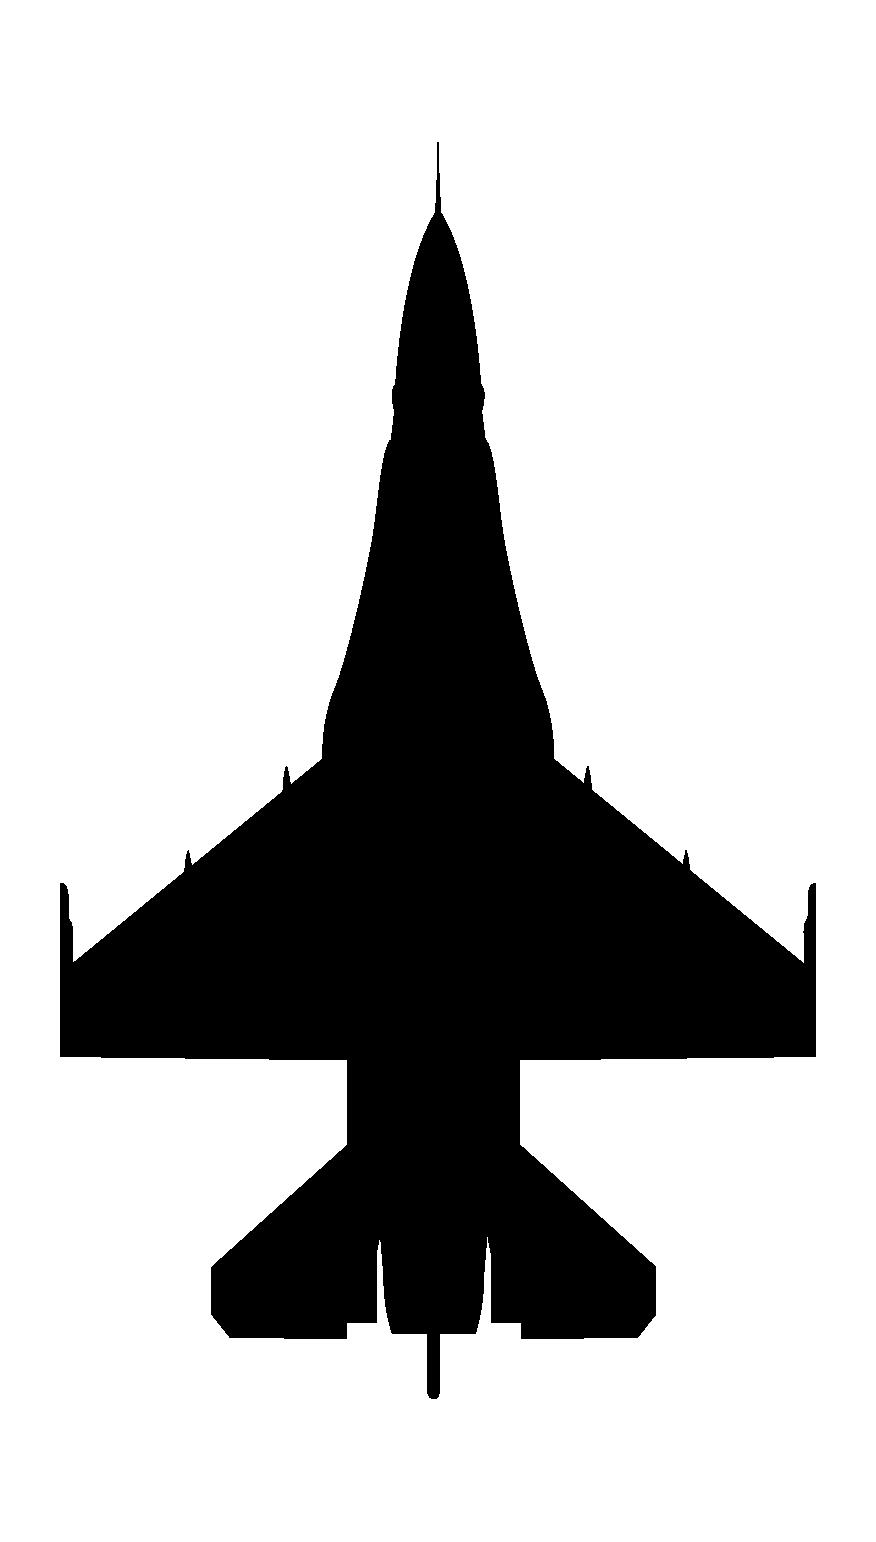
\includegraphics[
                    width=7.5mm,
            ]{diagrams/aircraft/silhouette_f16_top.pdf}};
    
        \end{tikzpicture}
        \caption{45 left}
    \end{subfigure}
    \caption{Tactical turn}
    \label{fig:aa_weap:form:tacturn}
\end{figure}

\begin{figure}[htbp]
    \centering
    \begin{tikzpicture}[figstyle]
            
        \draw[->] 
        (0,0) -- 
        node[below, pos=0]{
            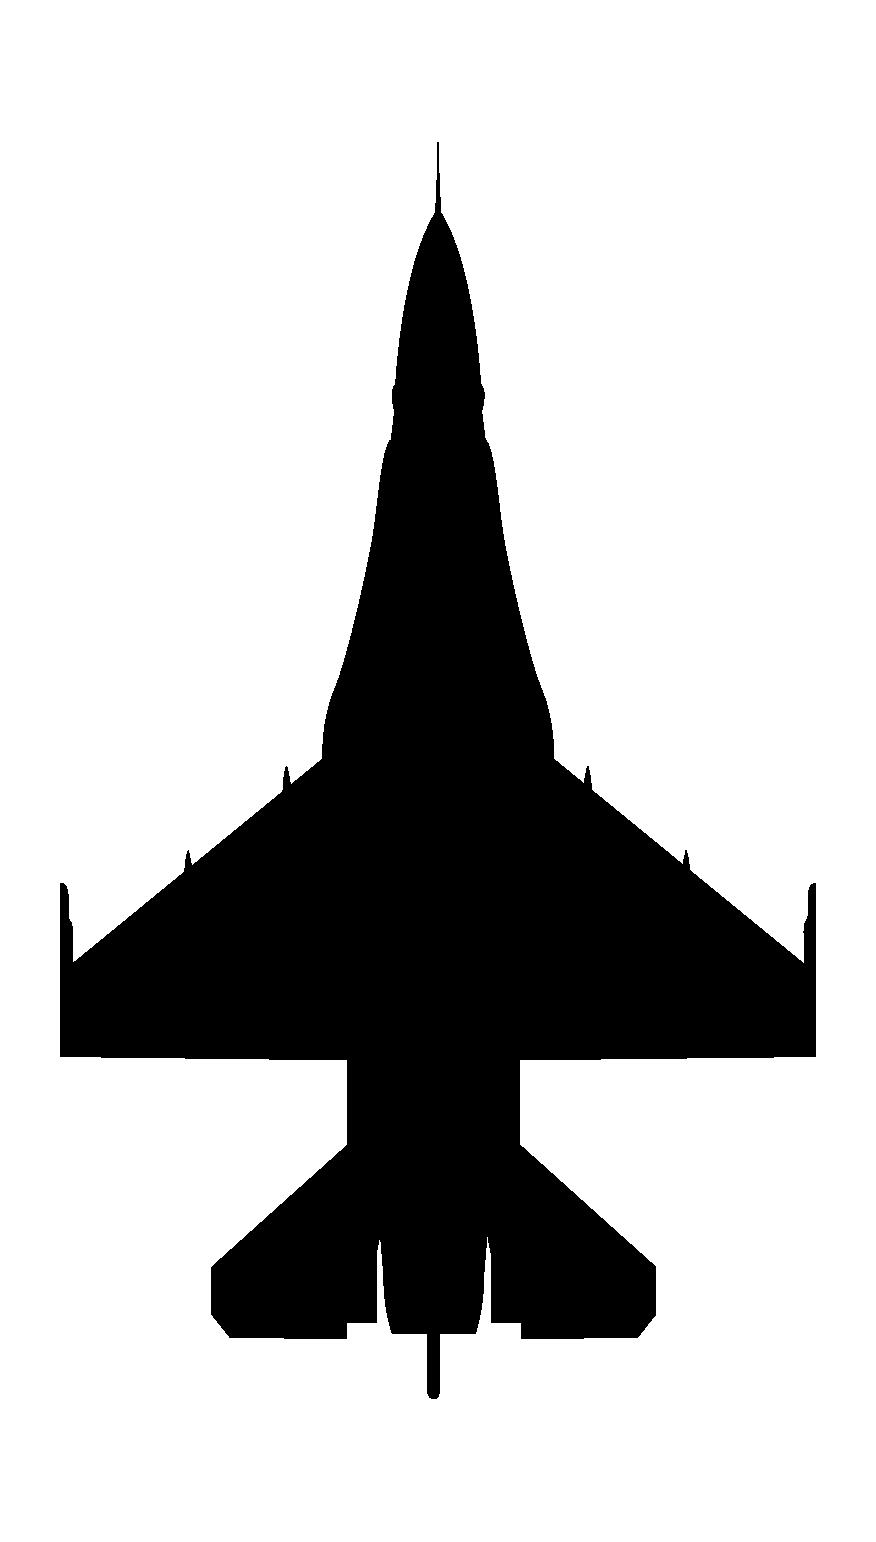
\includegraphics[
            width=7.5mm,
        ]{diagrams/aircraft/silhouette_f16_top.pdf}} 
        ++(0,20) 
        arc (180:00:10) 
        -- ++(0,-10)
        node[above, pos=1, rotate=180]{
            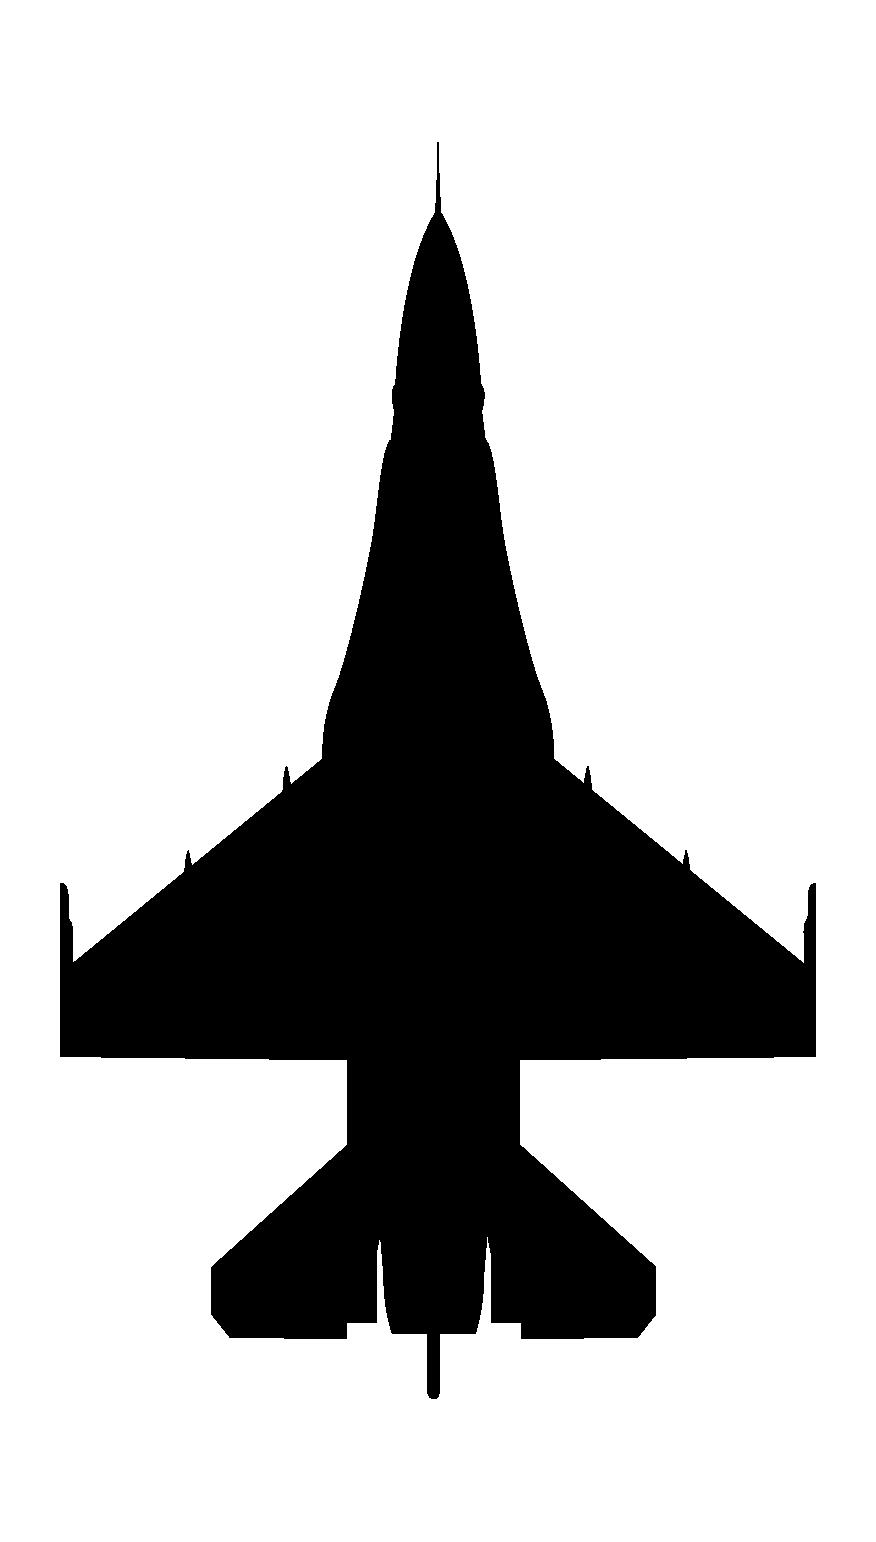
\includegraphics[
                width=7.5mm,
        ]{diagrams/aircraft/silhouette_f16_top.pdf}};
            
        \draw[->] 
        (10,0) -- 
        node[below, pos=0]{
            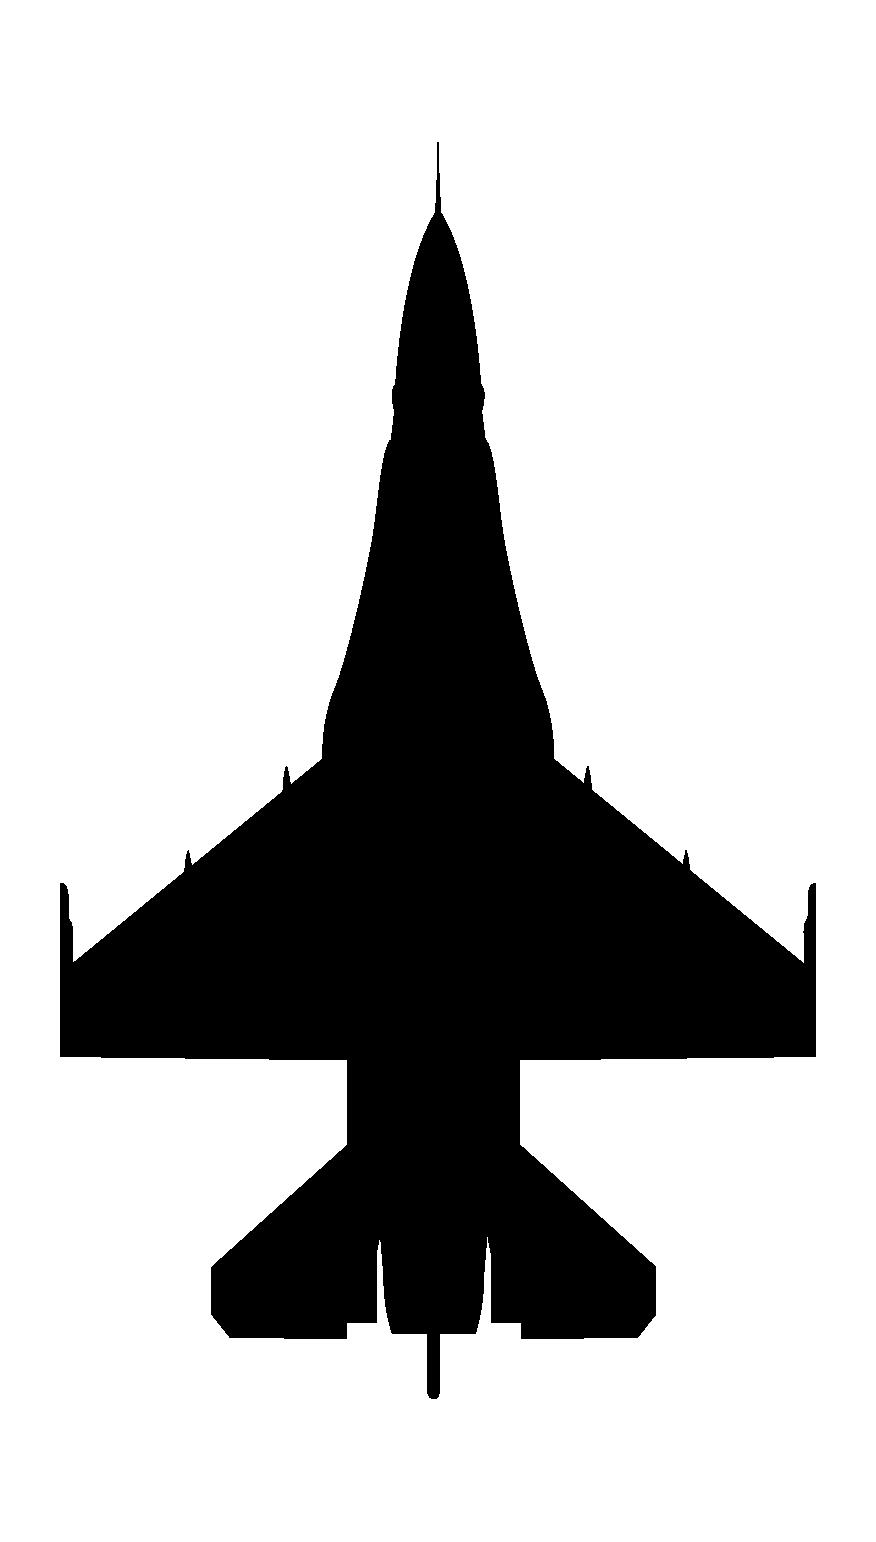
\includegraphics[
            width=7.5mm,
        ]{diagrams/aircraft/silhouette_f16_top.pdf}} 
        ++(0,20) 
        arc (180:0:10) 
        -- ++(0,-10)
        node[above, pos=1, rotate=180]{
            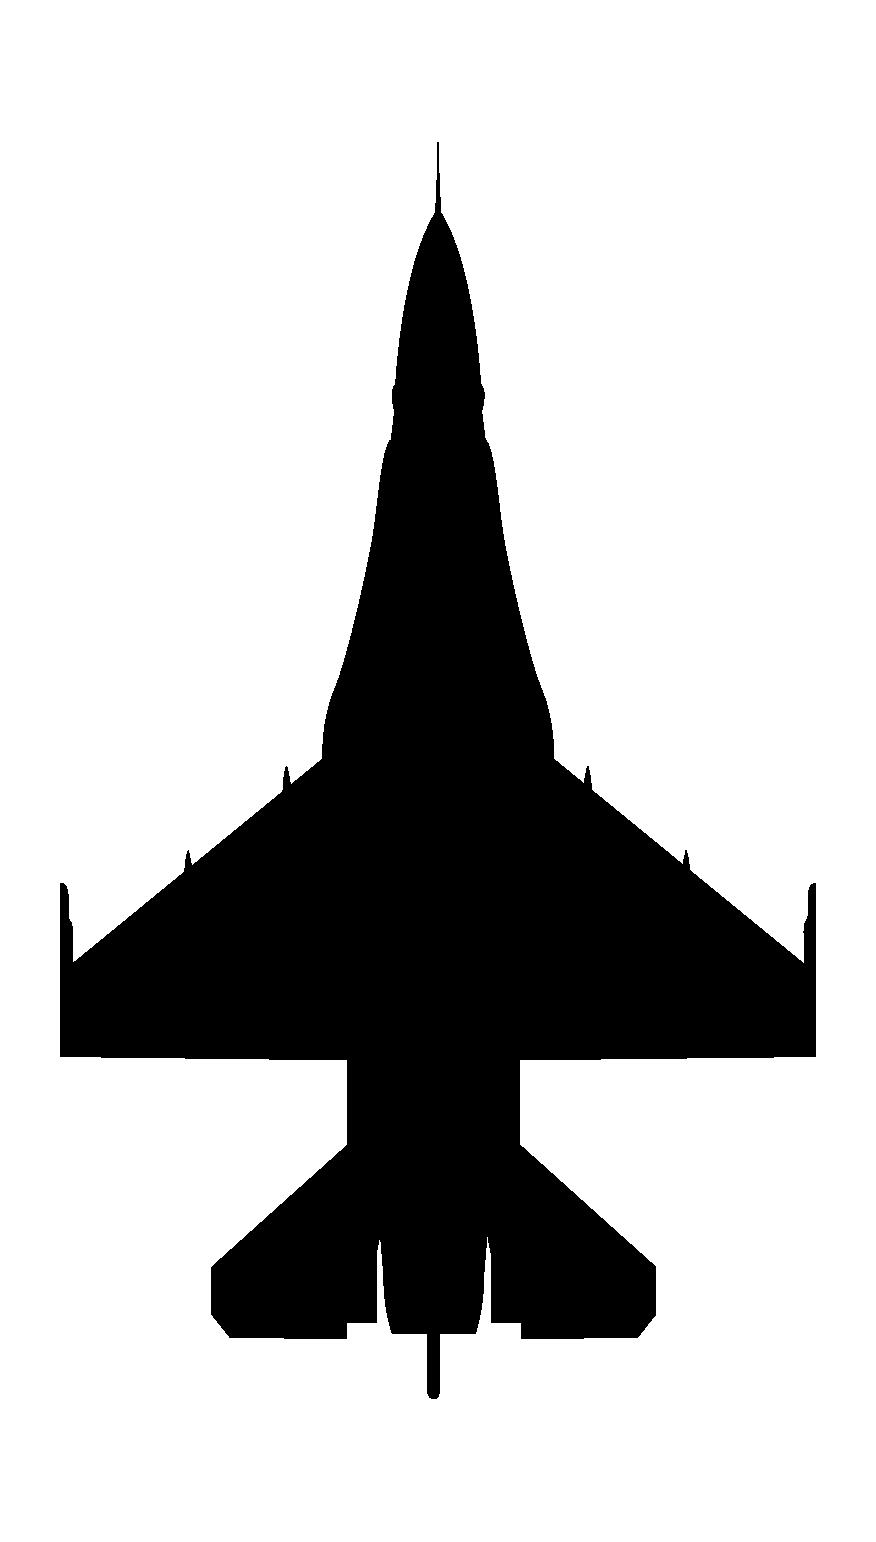
\includegraphics[
                width=7.5mm,
        ]{diagrams/aircraft/silhouette_f16_top.pdf}};

    \end{tikzpicture}
    \caption{Hook turn}
    \label{fig:aa_weap:form:hookturn}
\end{figure}

\begin{figure}[htbp]
    \centering
    \begin{tikzpicture}[figstyle]
            
        \draw[->] 
        (0,0) -- 
        node[below, pos=0]{
            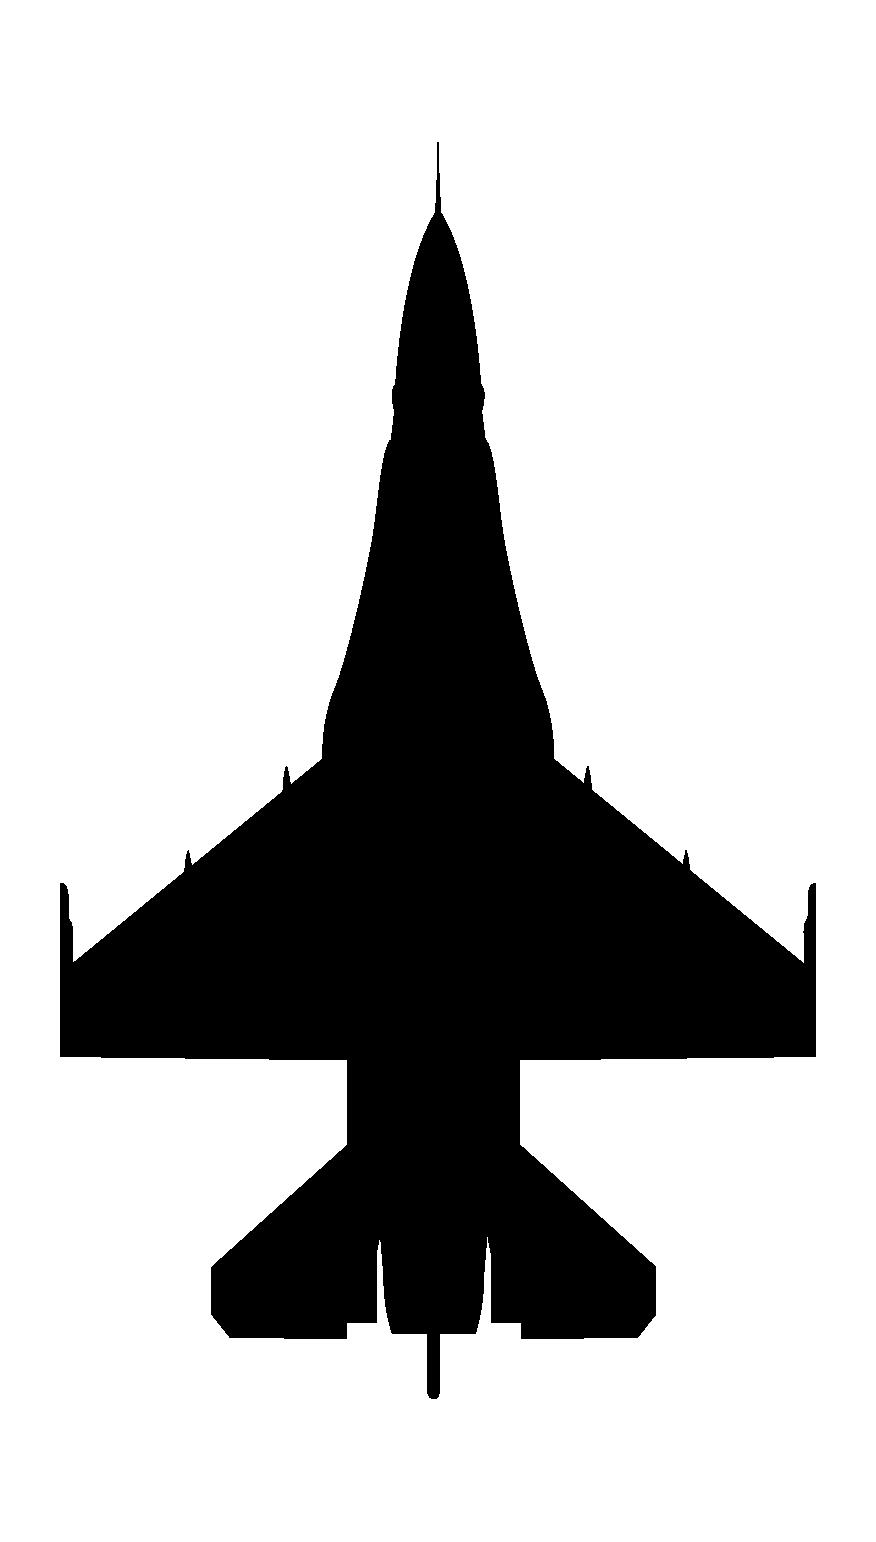
\includegraphics[
            width=7.5mm,
        ]{diagrams/aircraft/silhouette_f16_top.pdf}} 
        ++(0,20) 
        arc (180:00:10) 
        -- ++(0,-10)
        node[above, pos=1, rotate=180]{
            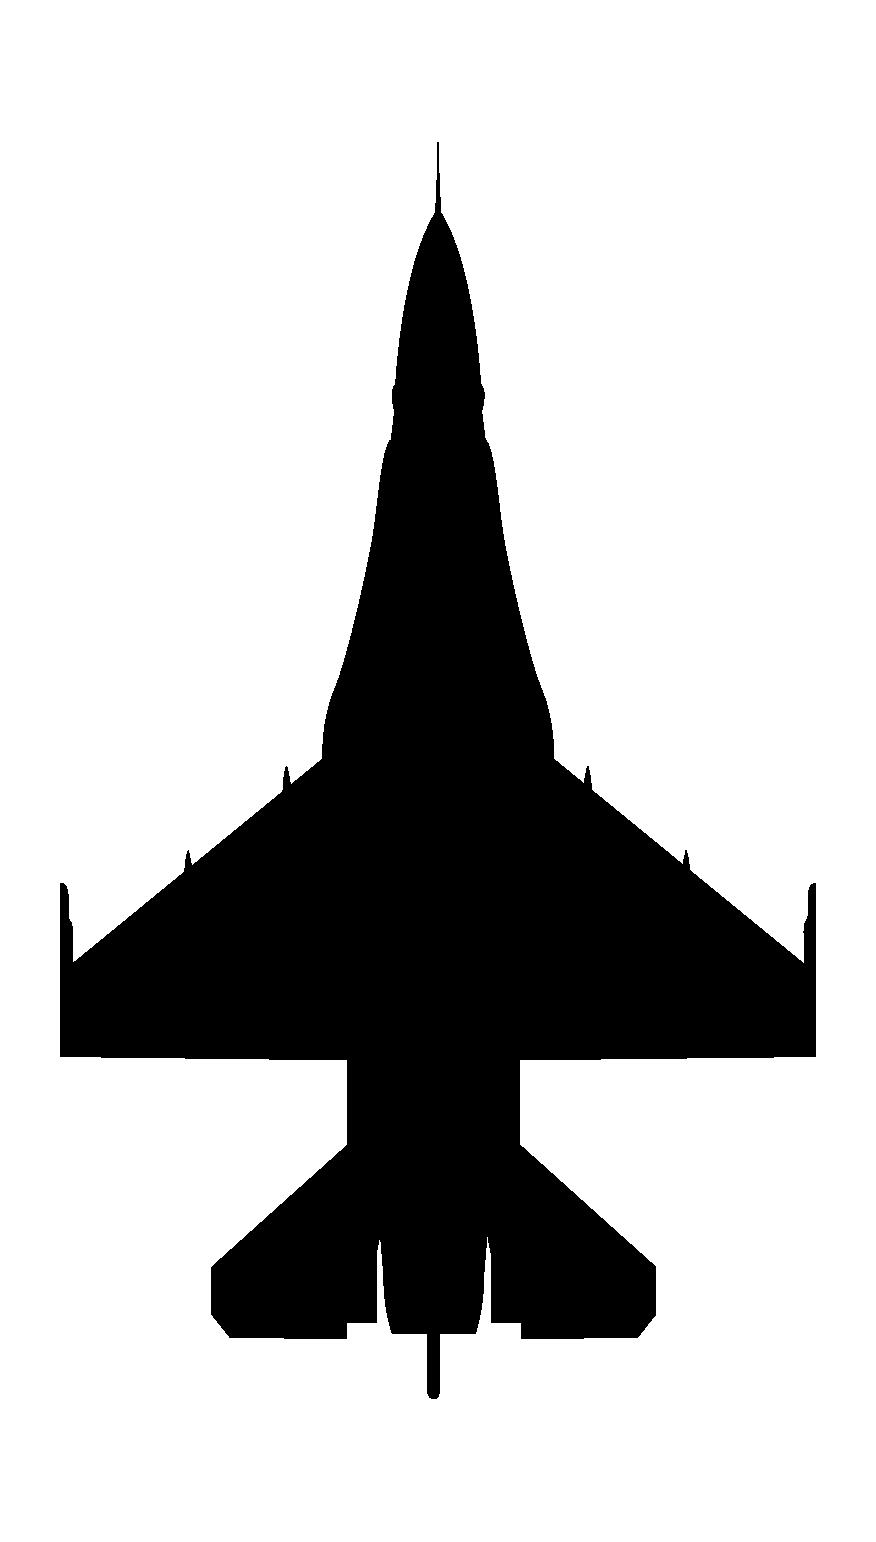
\includegraphics[
                width=7.5mm,
        ]{diagrams/aircraft/silhouette_f16_top.pdf}};
            
        \draw[->] 
        (10,0) -- 
        node[below, pos=0]{
            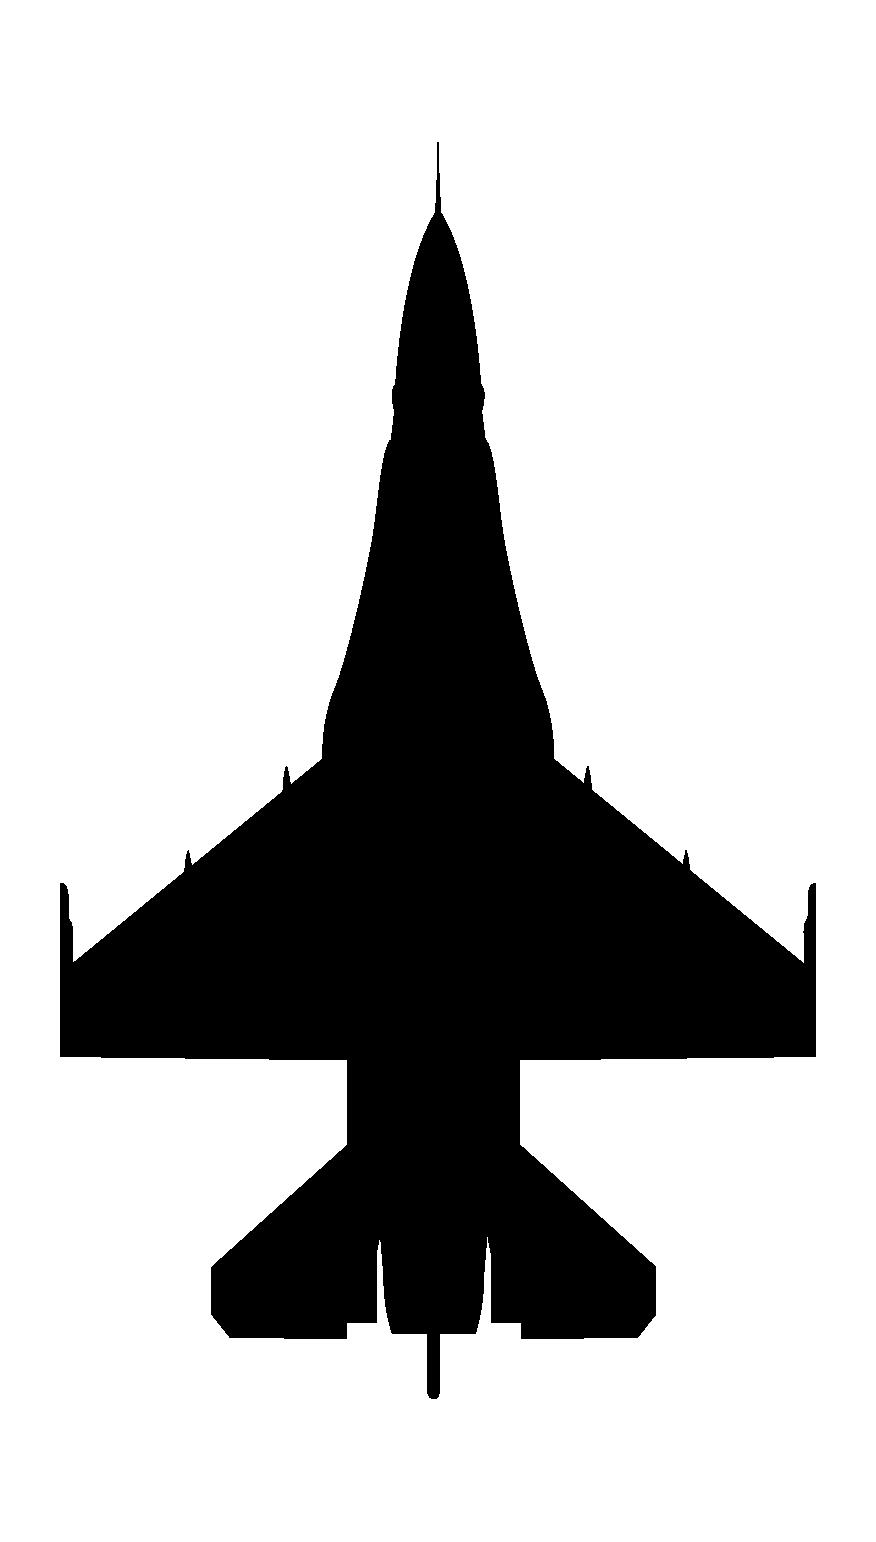
\includegraphics[
            width=7.5mm,
        ]{diagrams/aircraft/silhouette_f16_top.pdf}} 
        ++(0,20) 
        arc (0:180:10) 
        -- ++(0,-10)
        node[above, pos=1, rotate=180]{
            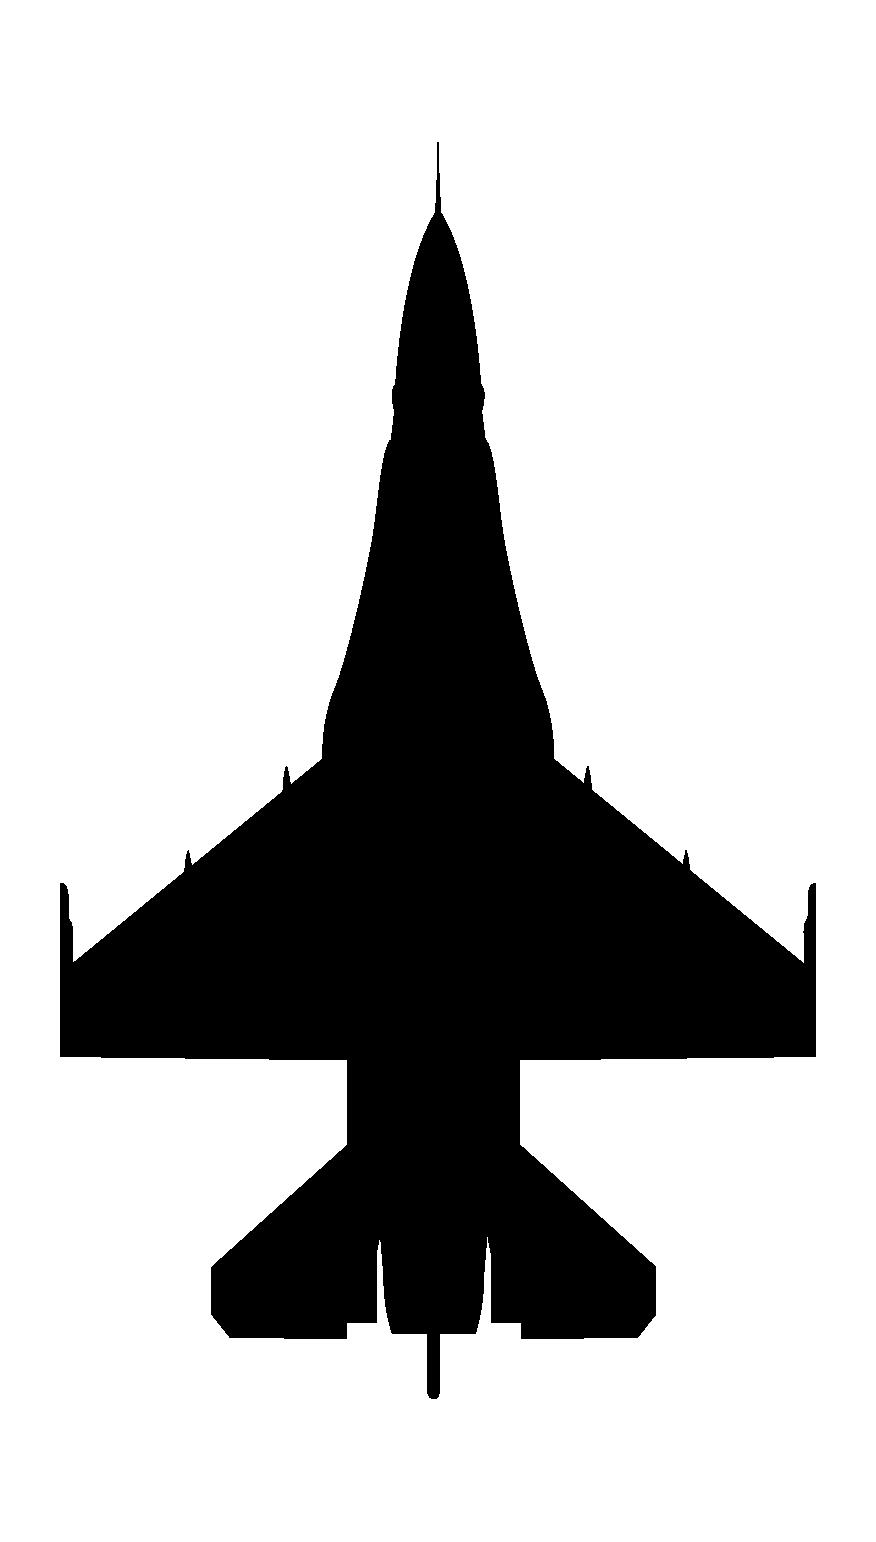
\includegraphics[
                width=7.5mm,
        ]{diagrams/aircraft/silhouette_f16_top.pdf}};

    \end{tikzpicture}
    \caption{Cross turn}
    \label{fig:aa_weap:form:crossturn}
\end{figure}

\begin{figure}[htbp]
    \centering
    \begin{tikzpicture}[figstyle]
            
        \draw[->] 
        (0,0) -- 
        node[below, pos=0]{
            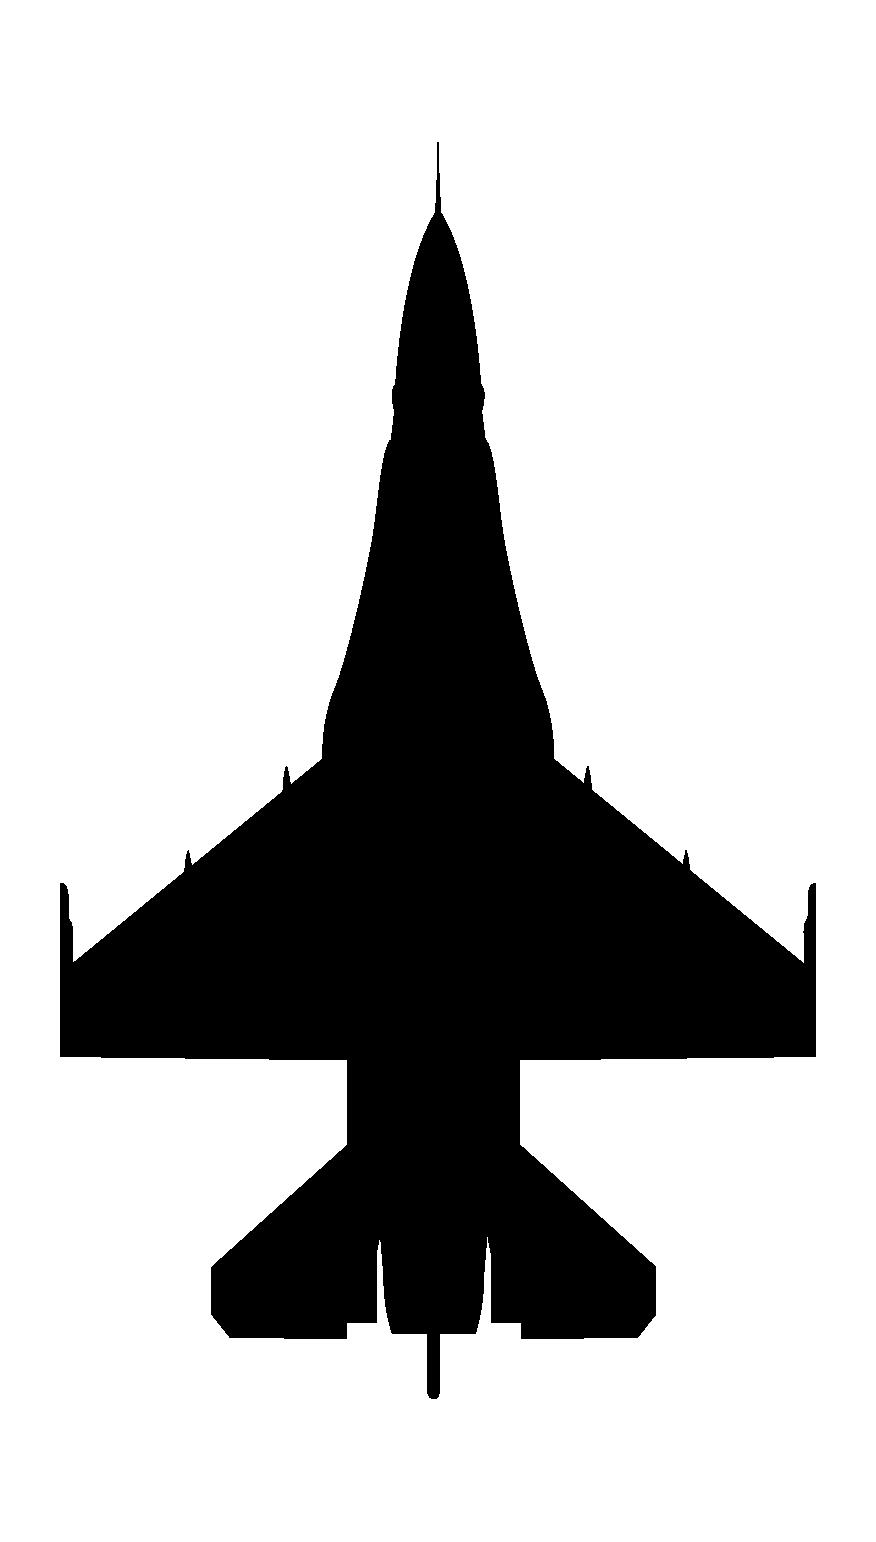
\includegraphics[
            width=7.5mm,
        ]{diagrams/aircraft/silhouette_f16_top.pdf}} 
        ++(0,5) 
        arc (180:135:17) 
        arc (-45:0:17) 
        -- ++(0,5)
        node[above, pos=1]{
            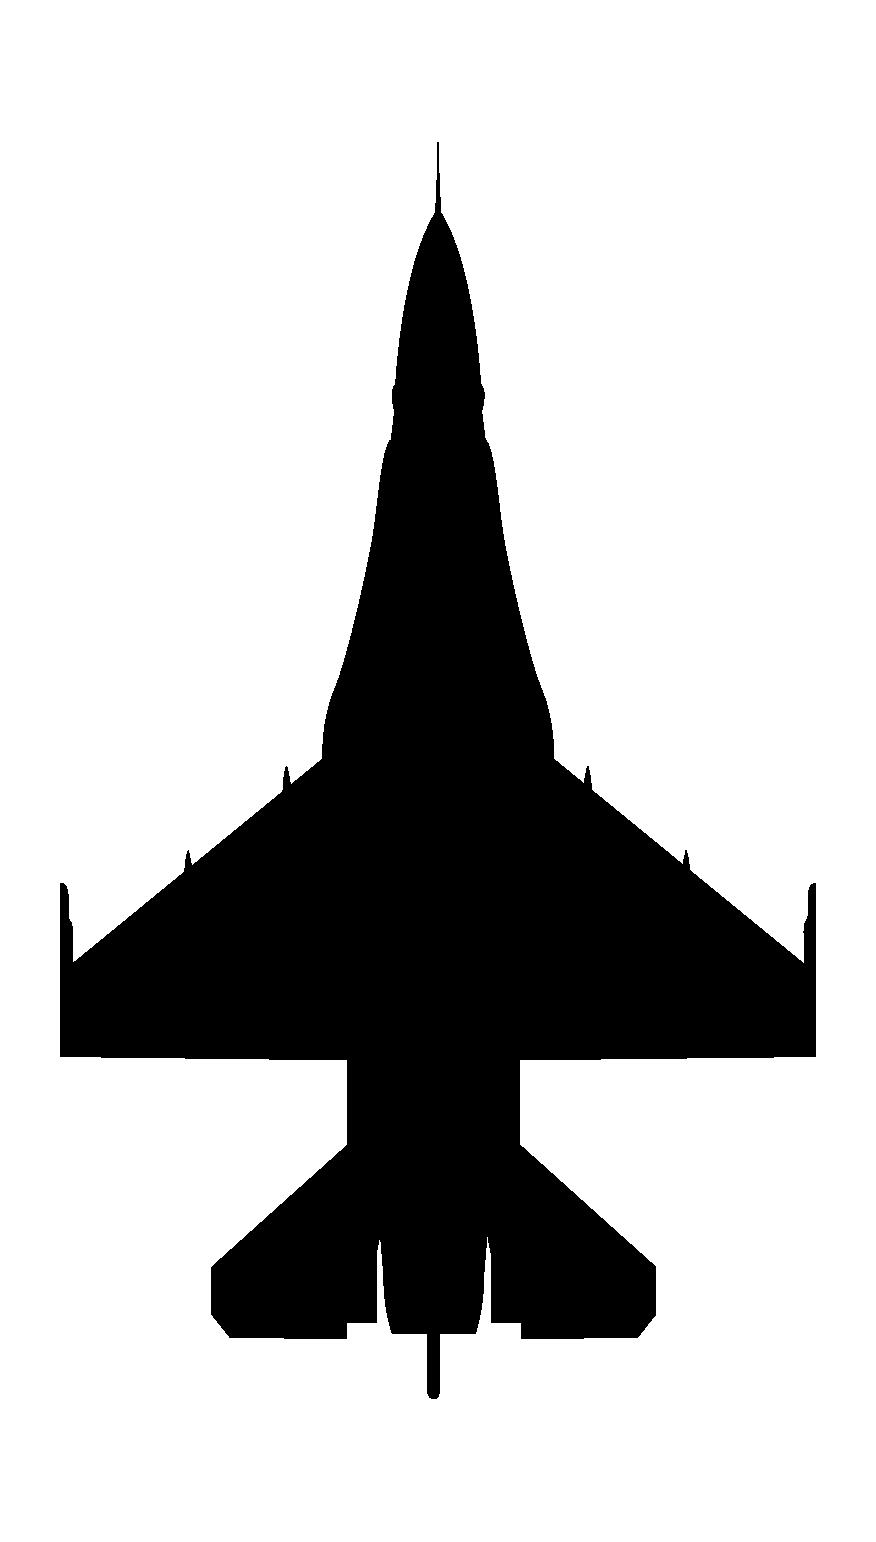
\includegraphics[
                width=7.5mm,
        ]{diagrams/aircraft/silhouette_f16_top.pdf}};
            
        \draw[->] 
        (10,0) -- 
        node[below, pos=0]{
            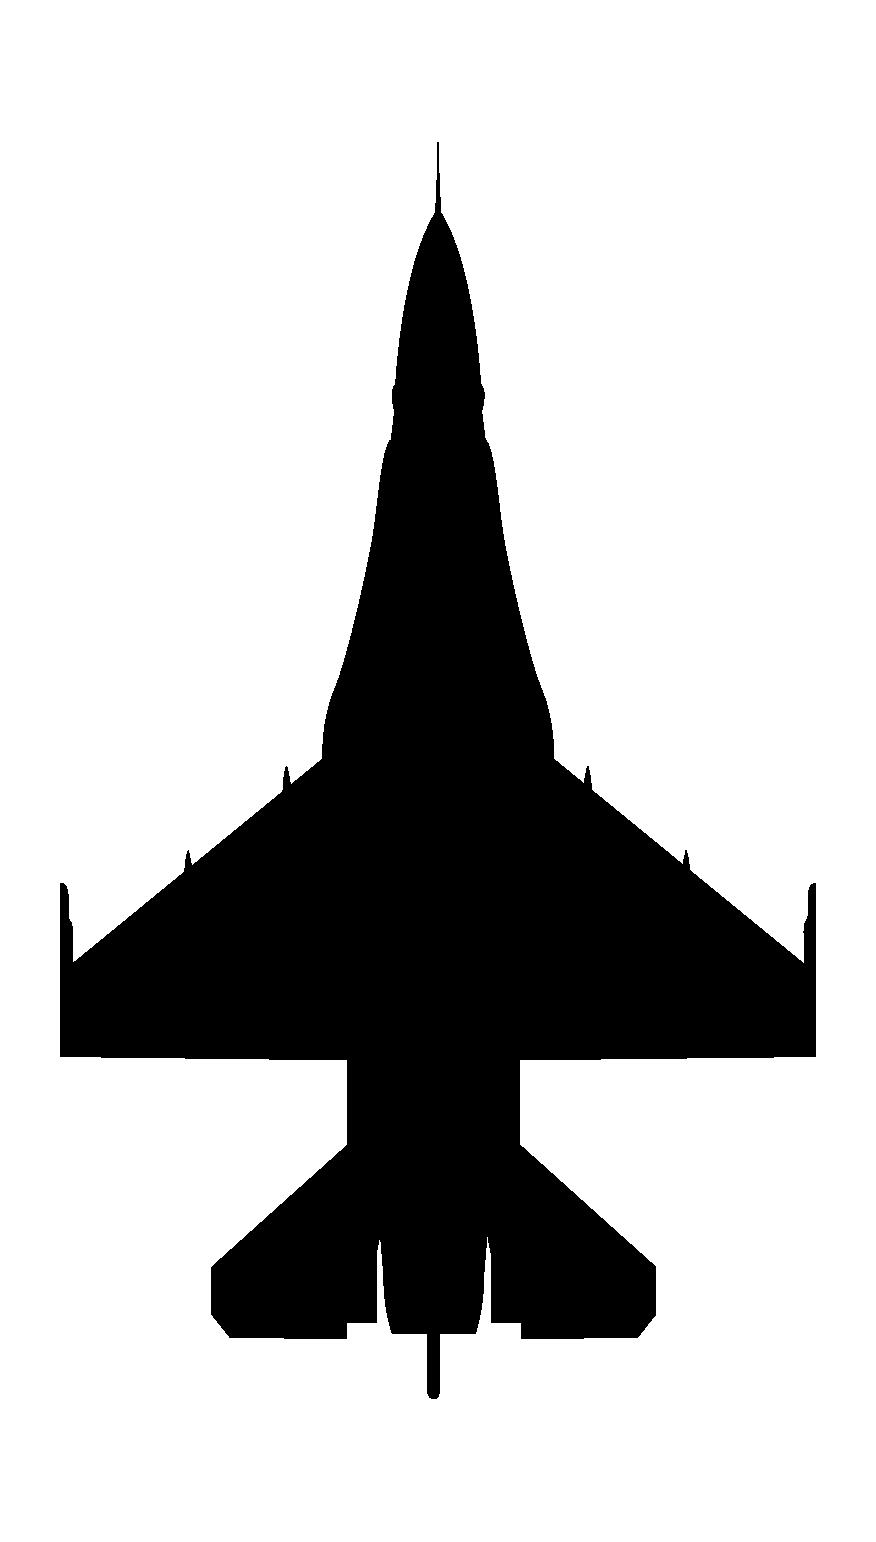
\includegraphics[
            width=7.5mm,
        ]{diagrams/aircraft/silhouette_f16_top.pdf}} 
        ++(0,5) 
        arc (0:45:17) 
        arc (-135:-180:17) 
        -- ++(0,5)
        node[above, pos=1]{
            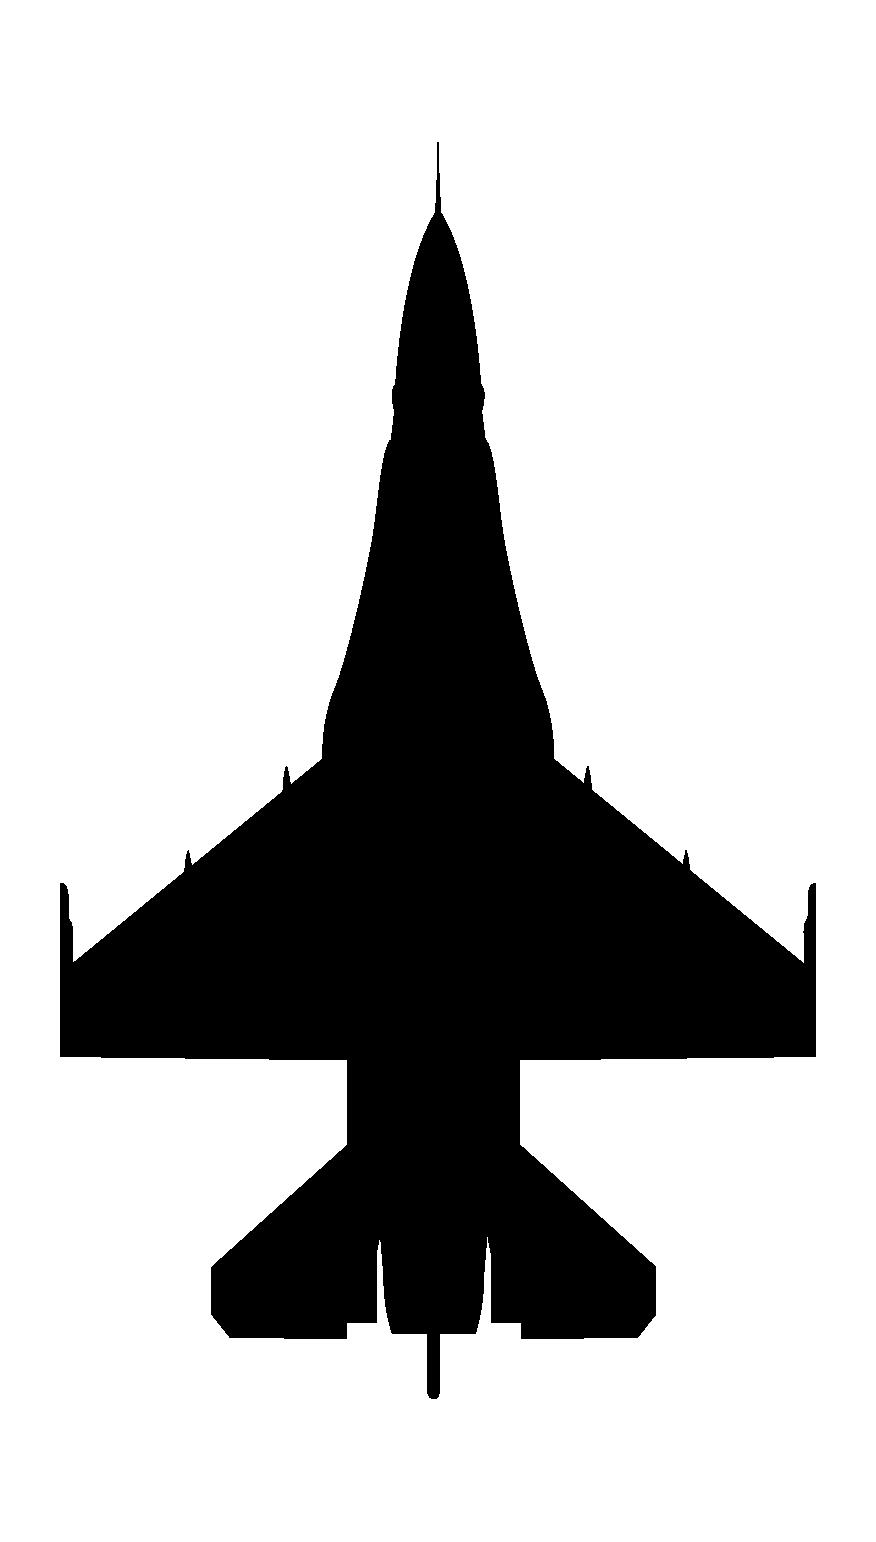
\includegraphics[
                width=7.5mm,
        ]{diagrams/aircraft/silhouette_f16_top.pdf}};

    \end{tikzpicture}
    \caption{Shackle}
    \label{fig:aa_weap:form:shackle}
\end{figure}

\clearpage

\subsection{FOUR-SHIP FORMATIONS}

\begin{figure}[htbp]
    \centering
    \begin{minipage}[b]{0.5\textwidth}
        \centering
        \begin{tikzpicture}[figstyle]
            
            \coordinate (1) at (0,0);
            \coordinate (2) at ($(1)+(20,0)$);
            \coordinate (3) at ($(1)+(0,-30)$);
            \coordinate (4) at ($(3)+(20,0)$);

            \draw[thin, <->]
            ($(1)+(-5,0)$) 
            -- ($(3)+(-5,0)$)
            node[font=\footnotesize, pos=0.5, rotate=90, above] {1.5-3.0 nm};
            \draw[thin]
            (1) -- ($(1)+(-7,0)$)
            (3) -- ($(3)+(-7,0)$);

            \draw[thin, <->]
            ($(1)+(0,5)$) 
            -- ($(2)+(0,5)$)
            node[font=\footnotesize, pos=0.5, above] {line abreast};
            \draw[thin]
            (1) -- ($(1)+(0,7)$)
            (2) -- ($(2)+(0,7)$);

            \draw[thin, <->]
            ($(3)+(0,5)$) 
            -- ($(4)+(0,5)$)
            node[font=\footnotesize, pos=0.5, above] {line abreast};
            \draw[thin]
            (3) -- ($(3)+(0,7)$)
            (4) -- ($(4)+(0,7)$);


            \node[yshift=-2mm] (1fig) at (1) {
                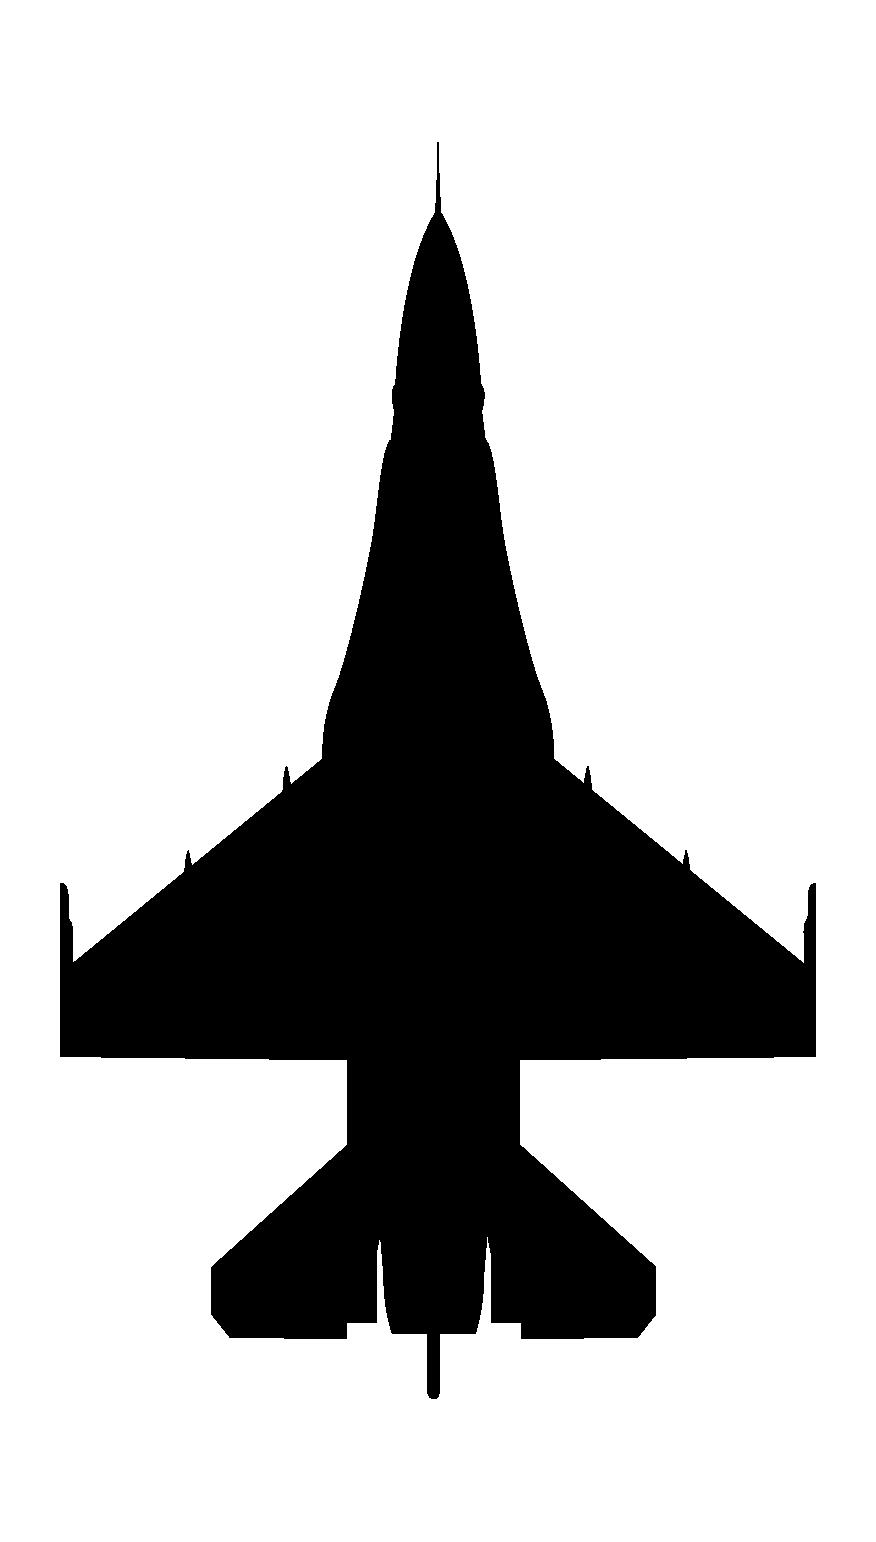
\includegraphics[
                    width=7.5mm,
                ]{diagrams/aircraft/silhouette_f16_top.pdf}
            };
            
            \node[yshift=-2mm] (2fig) at (2) {
                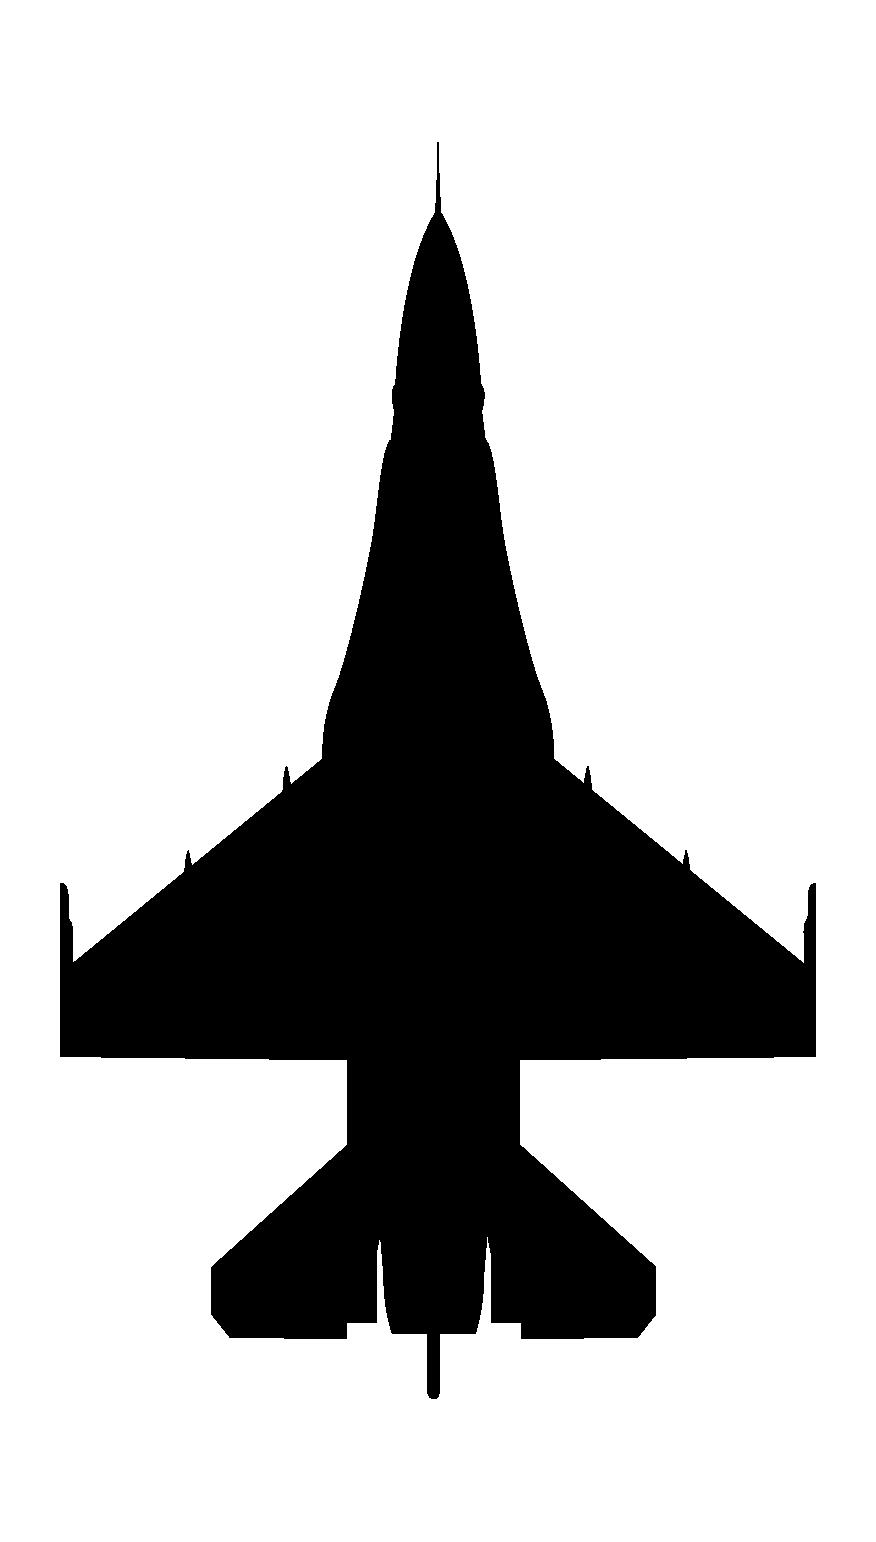
\includegraphics[
                    width=7.5mm,
                ]{diagrams/aircraft/silhouette_f16_top.pdf}
            };

            \node[yshift=-2mm] (3fig) at (3) {
                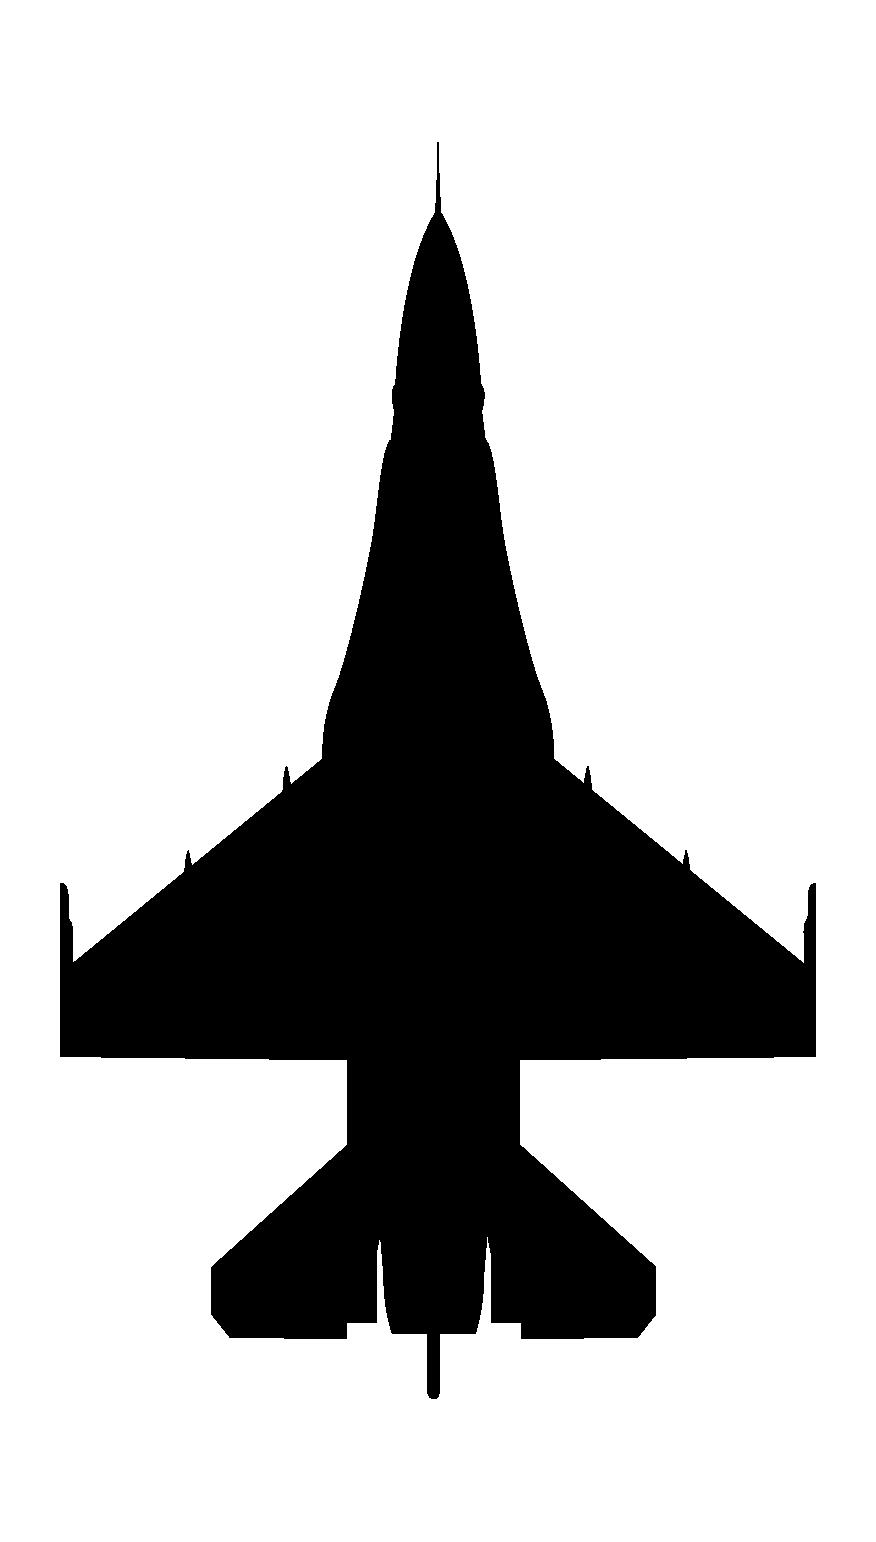
\includegraphics[
                    width=7.5mm,
                ]{diagrams/aircraft/silhouette_f16_top.pdf}
            };
            
            \node[yshift=-2mm] (4fig) at (4) {
                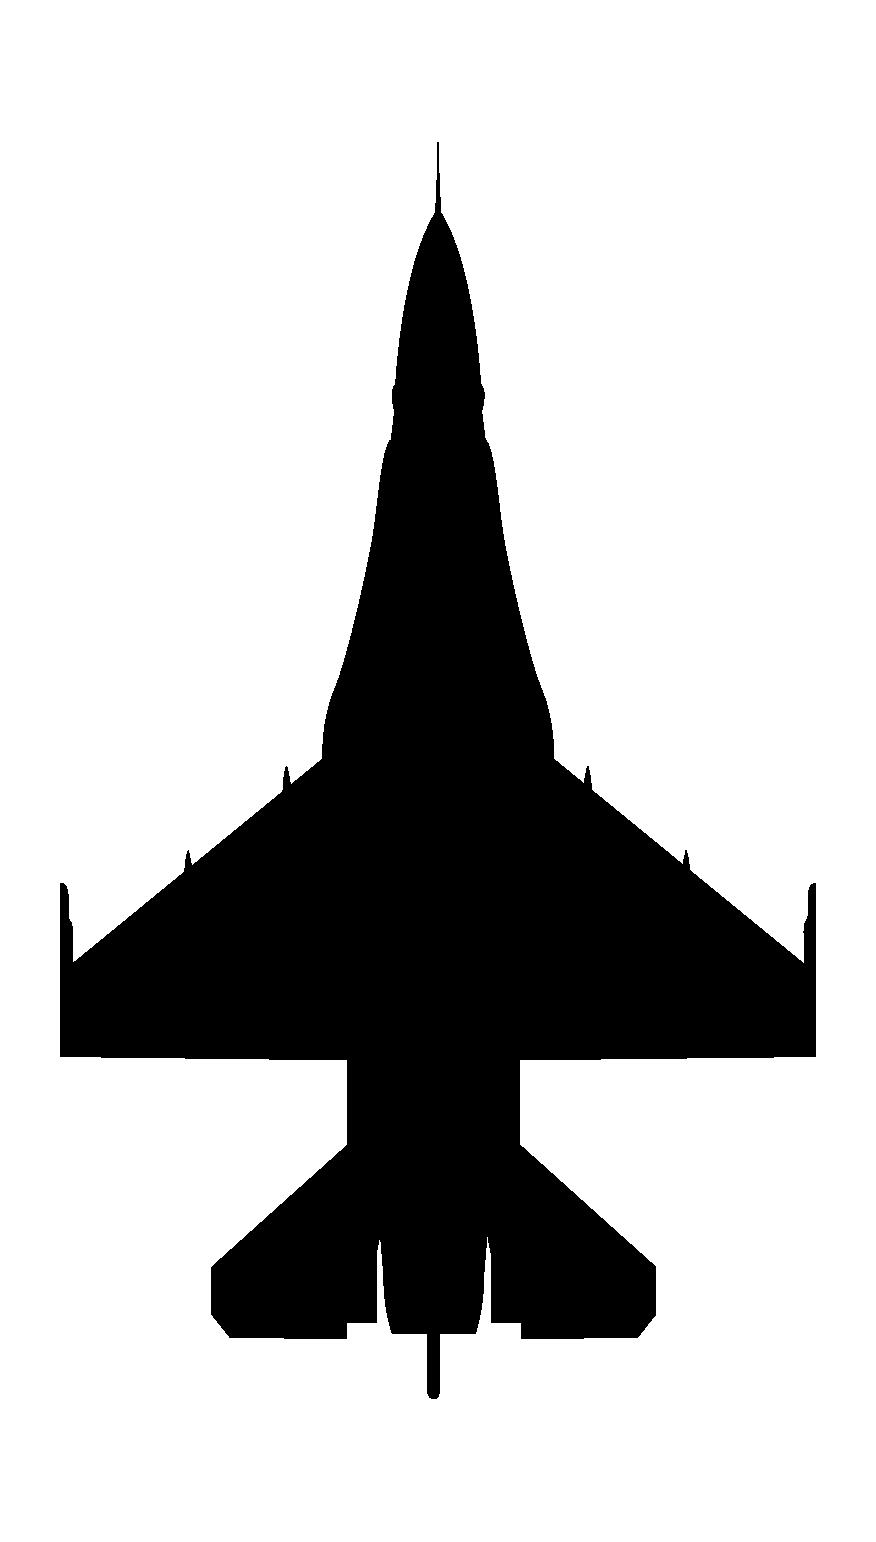
\includegraphics[
                    width=7.5mm,
                ]{diagrams/aircraft/silhouette_f16_top.pdf}
            };

            \node[anchor=north, font=\footnotesize] (1label) at (1fig.south) {1};
            \node[anchor=north, font=\footnotesize] (2label) at (2fig.south) {2};
            \node[anchor=north, font=\footnotesize] (3label) at (3fig.south) {3};
            \node[anchor=north, font=\footnotesize] (4label) at (4fig.south) {4};

        \end{tikzpicture}
        \caption{Four-ship box formation}
        \label{fig:aa_weap:form:box}
    \end{minipage}%
    \begin{minipage}[b]{0.5\textwidth}
        \centering
        \begin{tikzpicture}[figstyle]
            
            \coordinate (1) at (0,0);
            \coordinate (2) at ($(1)+(20,0)$);
            \coordinate (3) at ($(1)+(10,-30)$);
            \coordinate (4) at ($(3)+(20,0)$);

            \draw[thin, <->]
            ($(1)+(-5,0)$) 
            -- ($(3)+(-15,0)$)
            node[font=\footnotesize, pos=0.5, rotate=90, above] {1.5-3.0 nm};
            \draw[thin]
            (1) -- ($(1)+(-7,0)$)
            (3) -- ($(3)+(-17,0)$);

            \draw[thin, <->]
            ($(1)+(0,5)$) 
            -- ($(2)+(0,5)$)
            node[font=\footnotesize, pos=0.5, above] {line abreast};
            \draw[thin]
            (1) -- ($(1)+(0,7)$)
            (2) -- ($(2)+(0,7)$);

            \draw[thin, <->]
            ($(3)+(0,5)$) 
            -- ($(4)+(0,5)$)
            node[font=\footnotesize, pos=0.5, above] {line abreast};
            \draw[thin]
            (3) -- ($(3)+(0,7)$)
            (4) -- ($(4)+(0,7)$);


            \node[yshift=-2mm] (1fig) at (1) {
                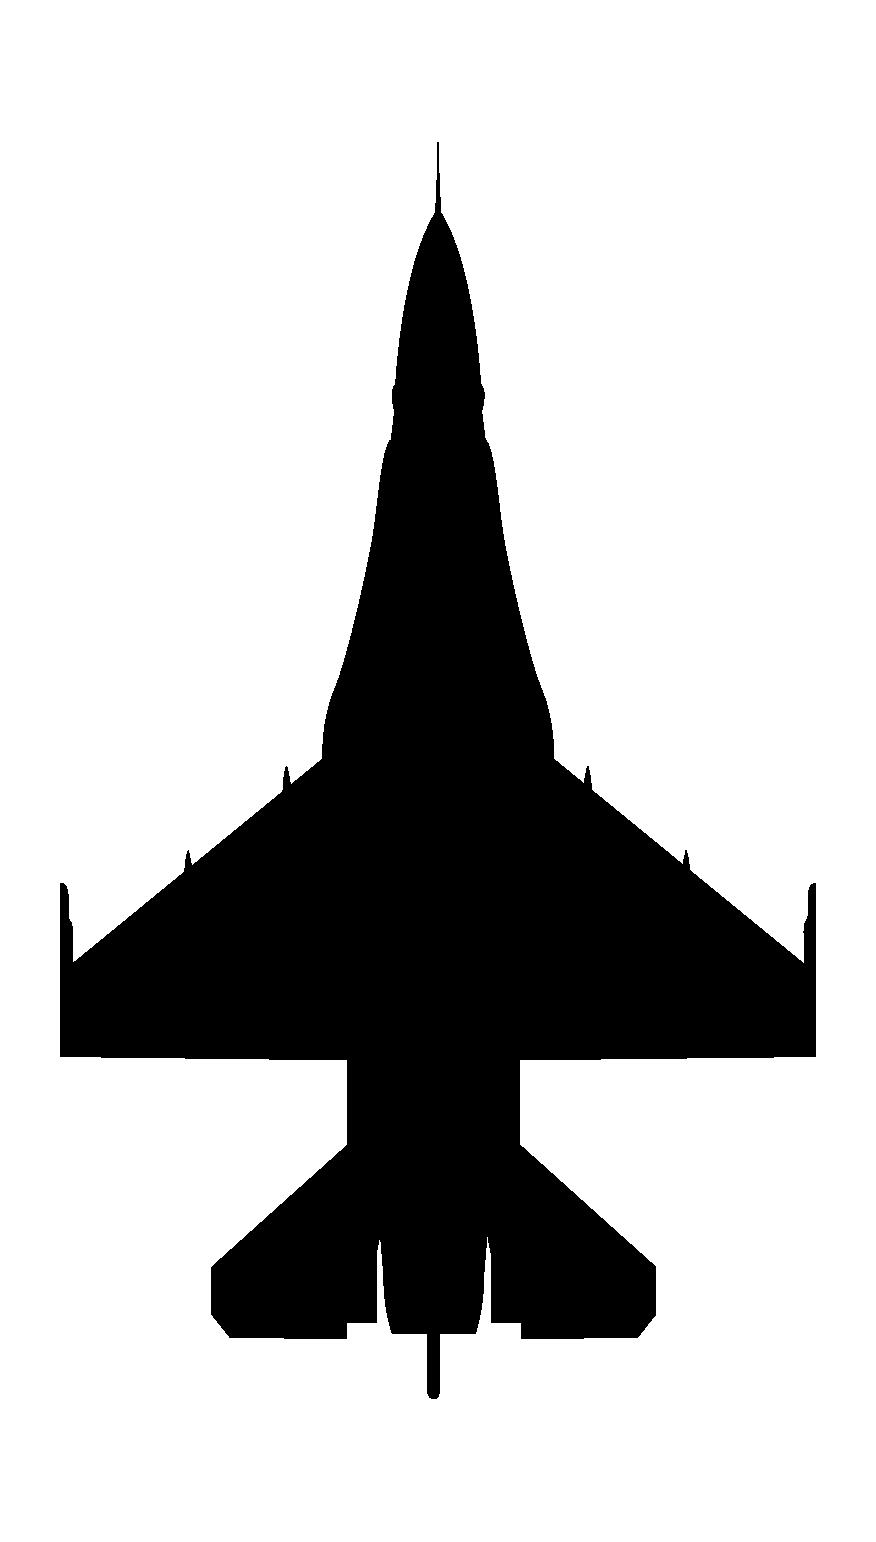
\includegraphics[
                    width=7.5mm,
                ]{diagrams/aircraft/silhouette_f16_top.pdf}
            };
            
            \node[yshift=-2mm] (2fig) at (2) {
                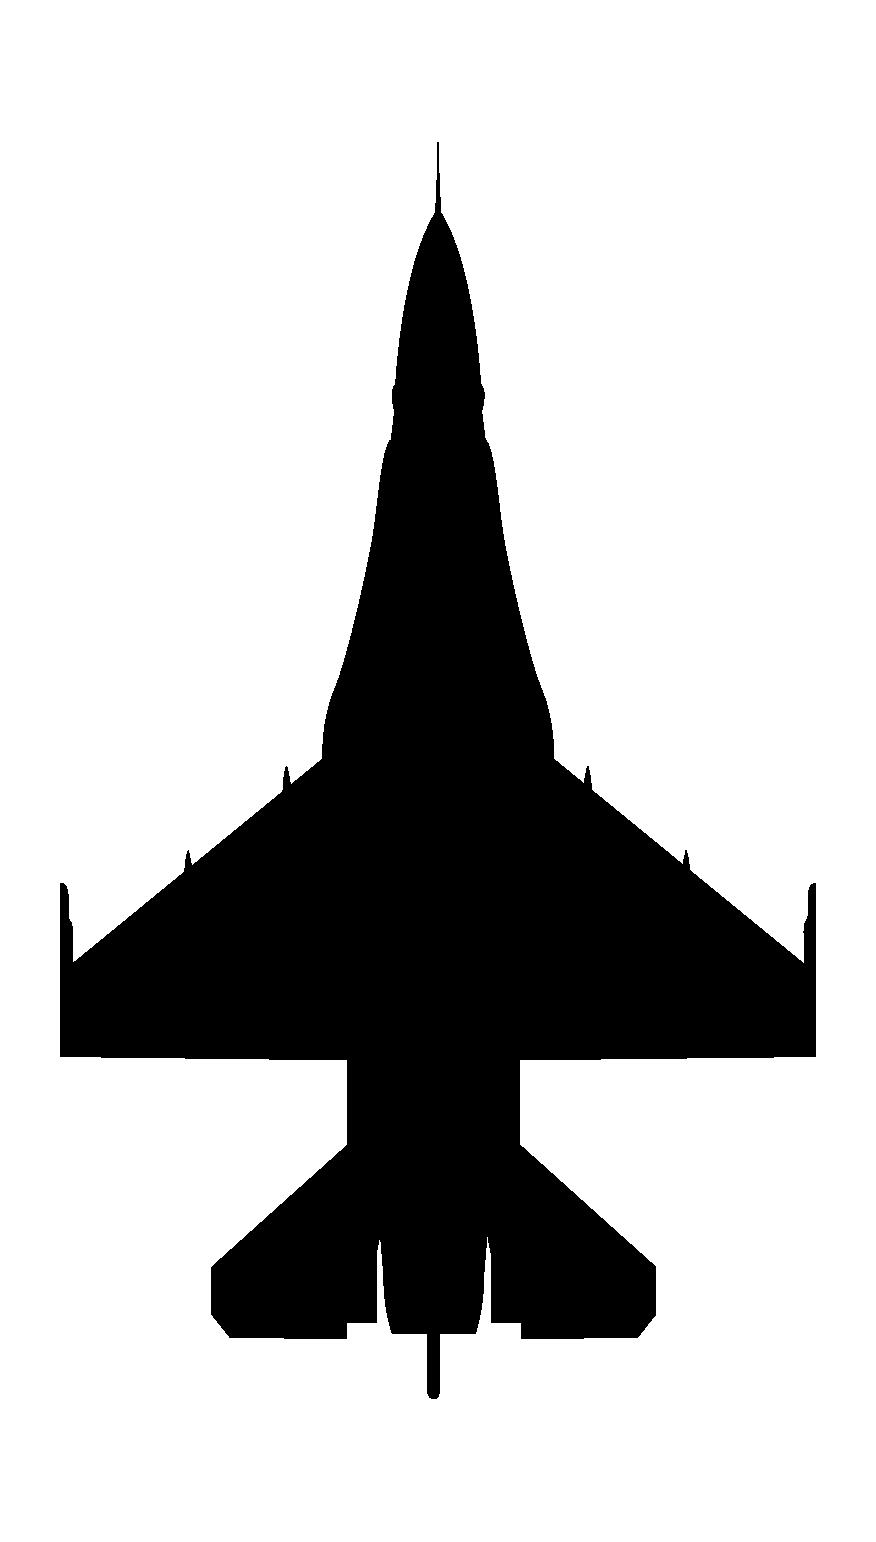
\includegraphics[
                    width=7.5mm,
                ]{diagrams/aircraft/silhouette_f16_top.pdf}
            };

            \node[yshift=-2mm] (3fig) at (3) {
                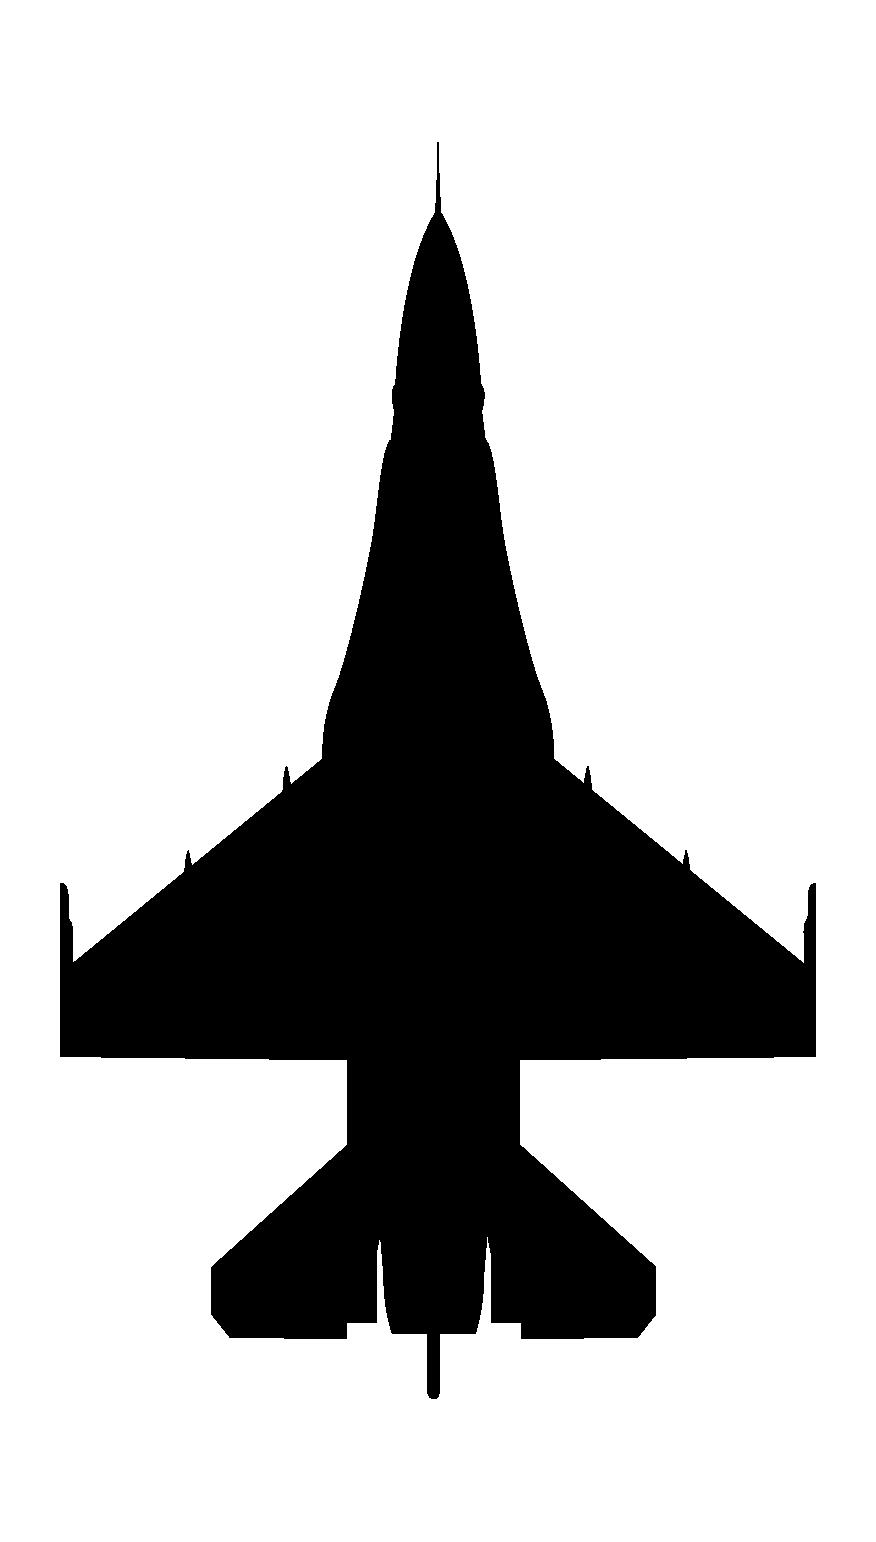
\includegraphics[
                    width=7.5mm,
                ]{diagrams/aircraft/silhouette_f16_top.pdf}
            };
            
            \node[yshift=-2mm] (4fig) at (4) {
                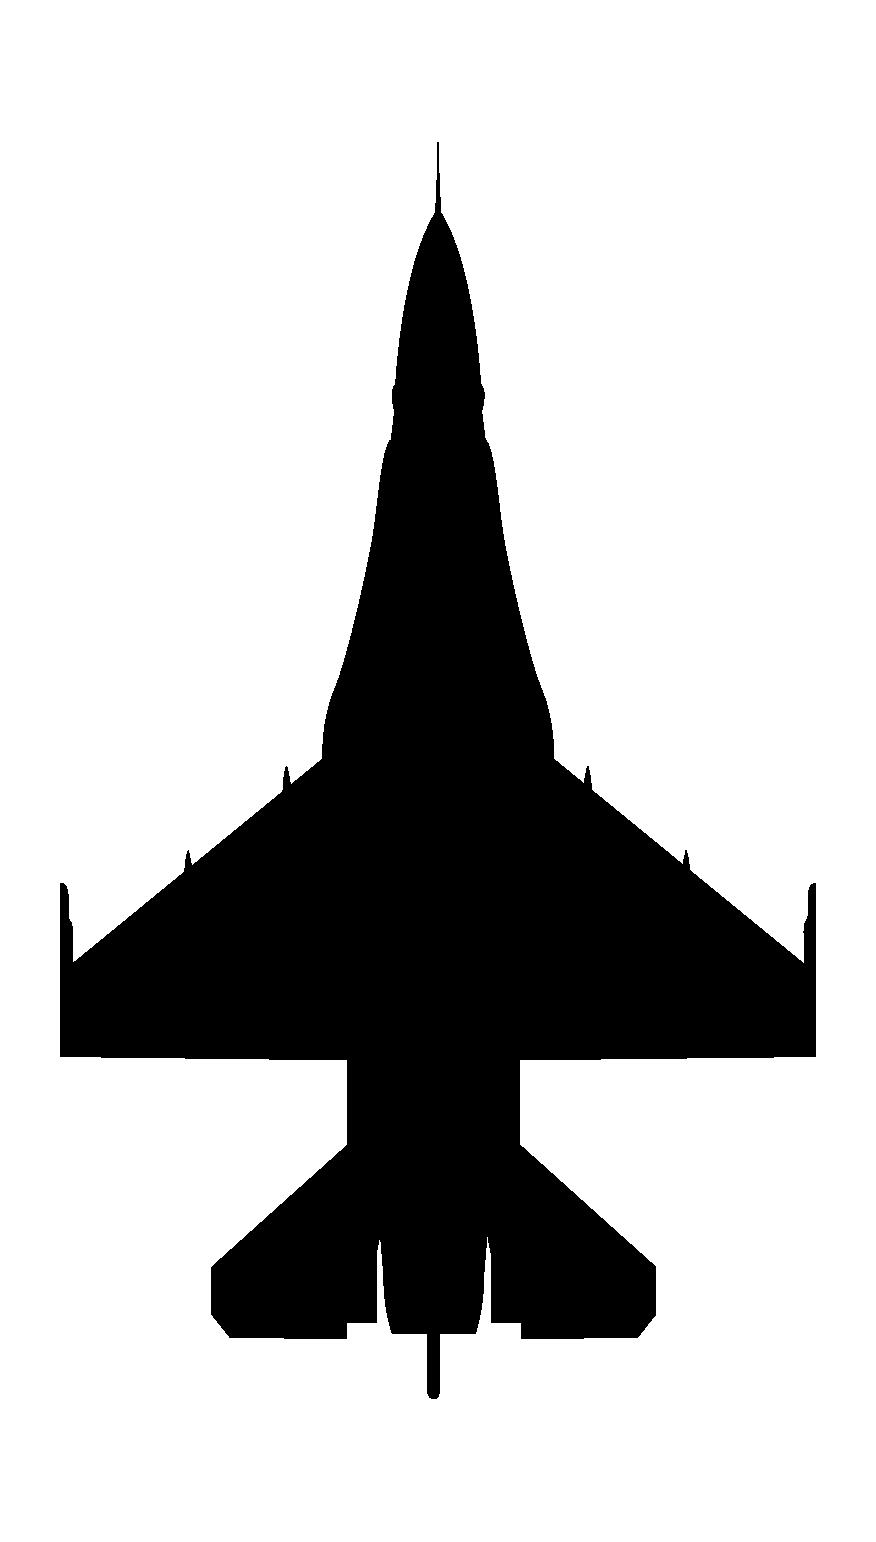
\includegraphics[
                    width=7.5mm,
                ]{diagrams/aircraft/silhouette_f16_top.pdf}
            };

            \node[anchor=north, font=\footnotesize] (1label) at (1fig.south) {1};
            \node[anchor=north, font=\footnotesize] (2label) at (2fig.south) {2};
            \node[anchor=north, font=\footnotesize] (3label) at (3fig.south) {3};
            \node[anchor=north, font=\footnotesize] (4label) at (4fig.south) {4};

        \end{tikzpicture}
        \caption{Four-ship offset box formation}
        \label{fig:aa_weap:form:boxoffset}
    \end{minipage}
\end{figure}

\begin{figure}[htbp]
    \centering
    \begin{tikzpicture}[figstyle]
        
        \coordinate (1) at (0,0);
        \coordinate (2) at ($(1)+(-135:20)$);
        \coordinate (3) at ($(1)+(20,0)$);
        \coordinate (4) at ($(3)+(-45:20)$);

        \draw[thin]
        (1) -- (2) node[font=\footnotesize, pos=0.5, above left] {fighting wing}
        (3) -- (4)node[font=\footnotesize, pos=0.5, above right] {fighting wing};

        \draw[thin, <->]
        ($(1)+(0,5)$) 
        -- ($(3)+(0,5)$)
        node[font=\footnotesize, pos=0.5, above] {line abreast};
        \draw[thin]
        (1) -- ($(1)+(0,7)$)
        (3) -- ($(3)+(0,7)$);

        \node[yshift=-2mm] (1fig) at (1) {
            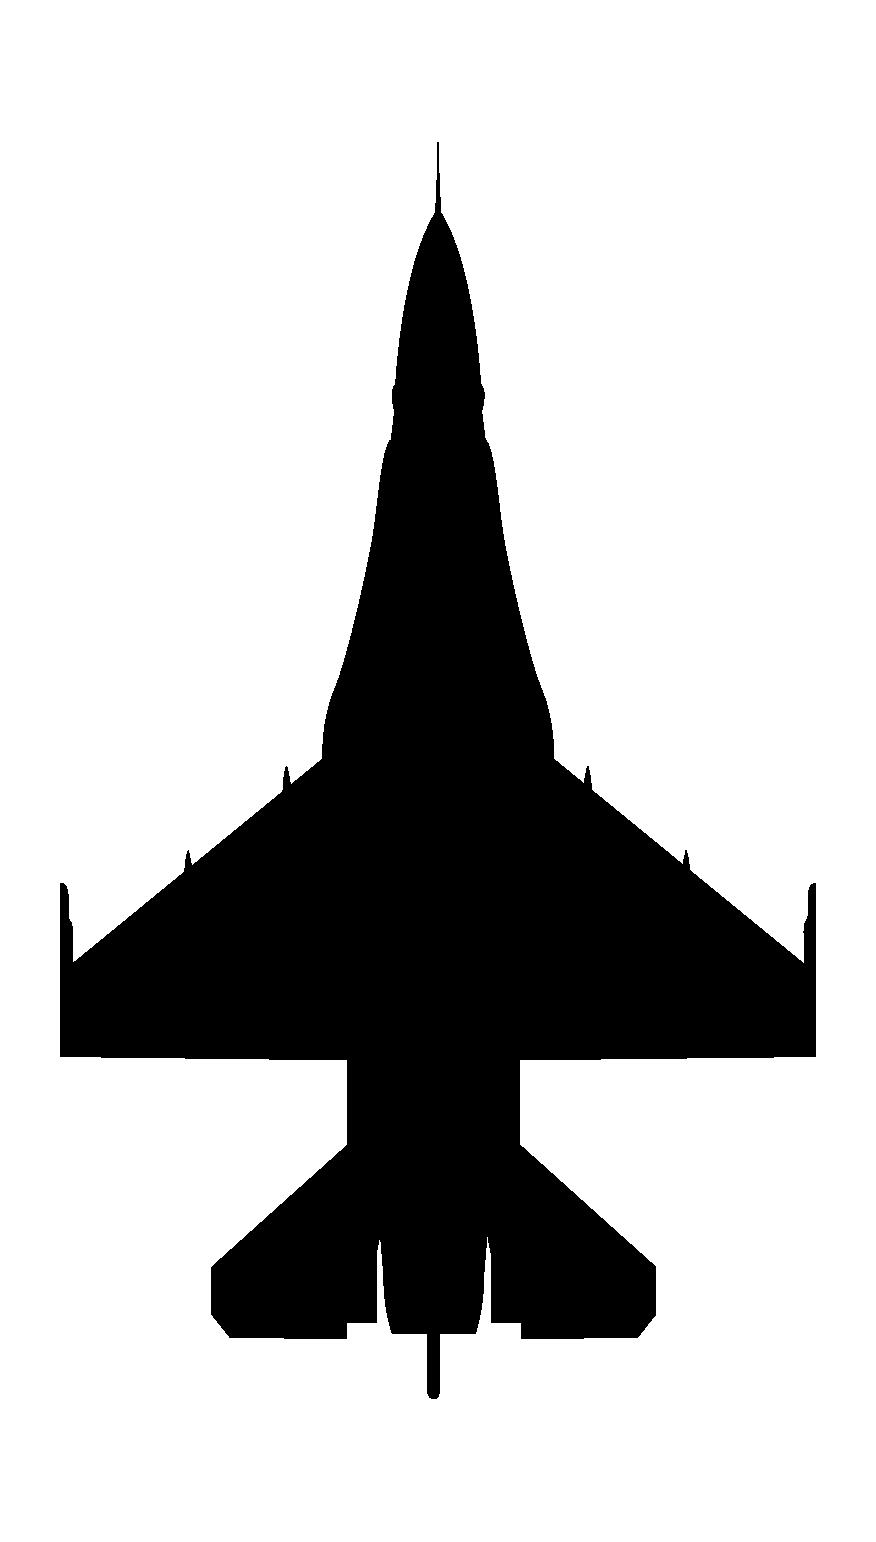
\includegraphics[
                width=7.5mm,
            ]{diagrams/aircraft/silhouette_f16_top.pdf}
        };
        
        \node[yshift=-2mm] (2fig) at (2) {
            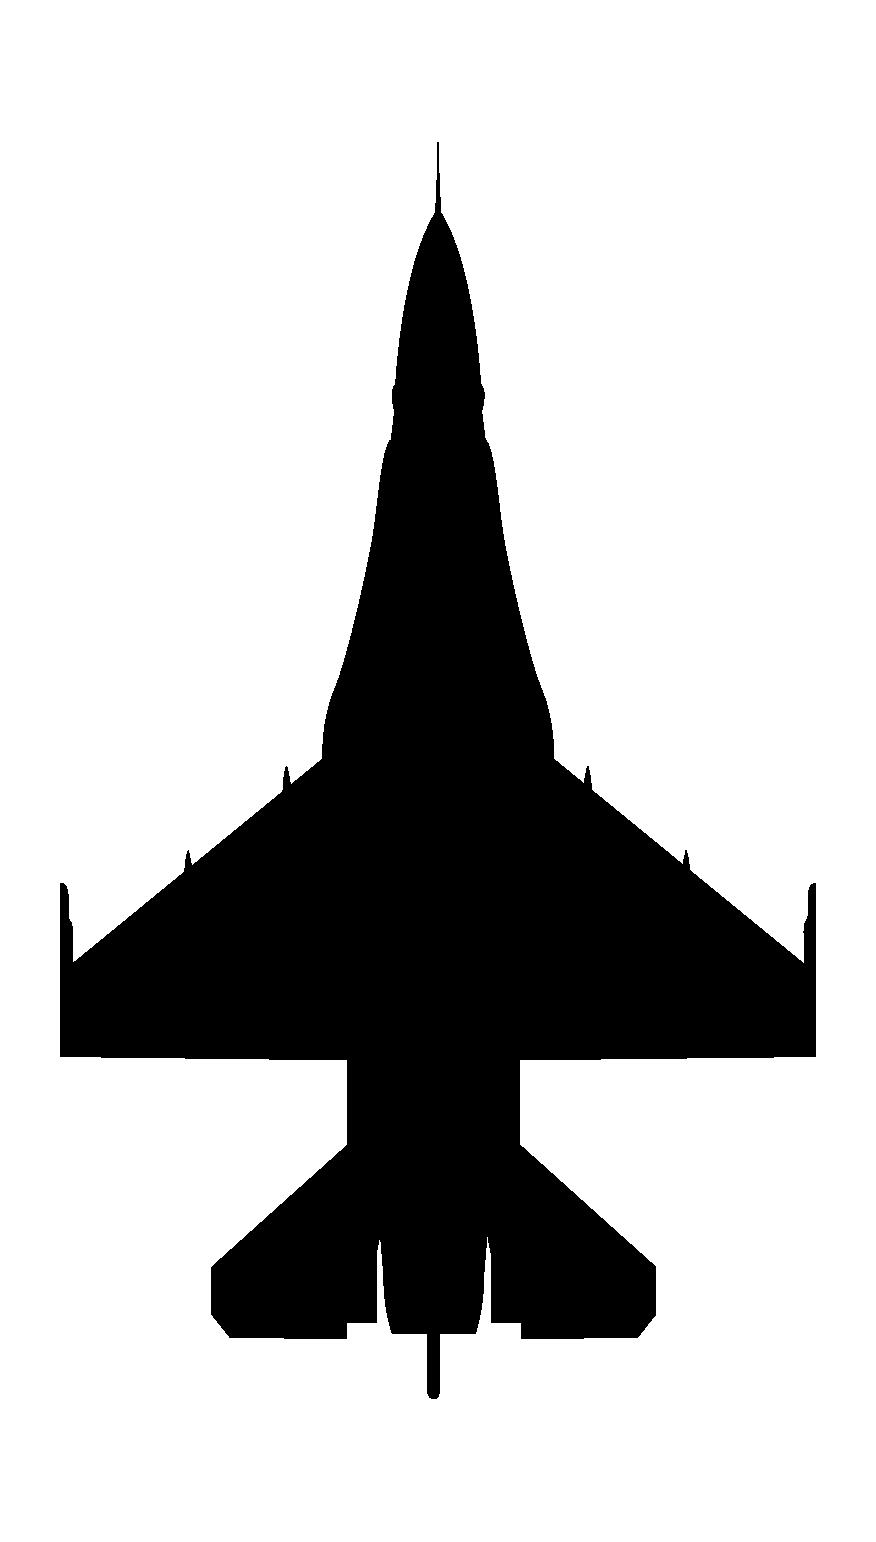
\includegraphics[
                width=7.5mm,
            ]{diagrams/aircraft/silhouette_f16_top.pdf}
        };

        \node[yshift=-2mm] (3fig) at (3) {
            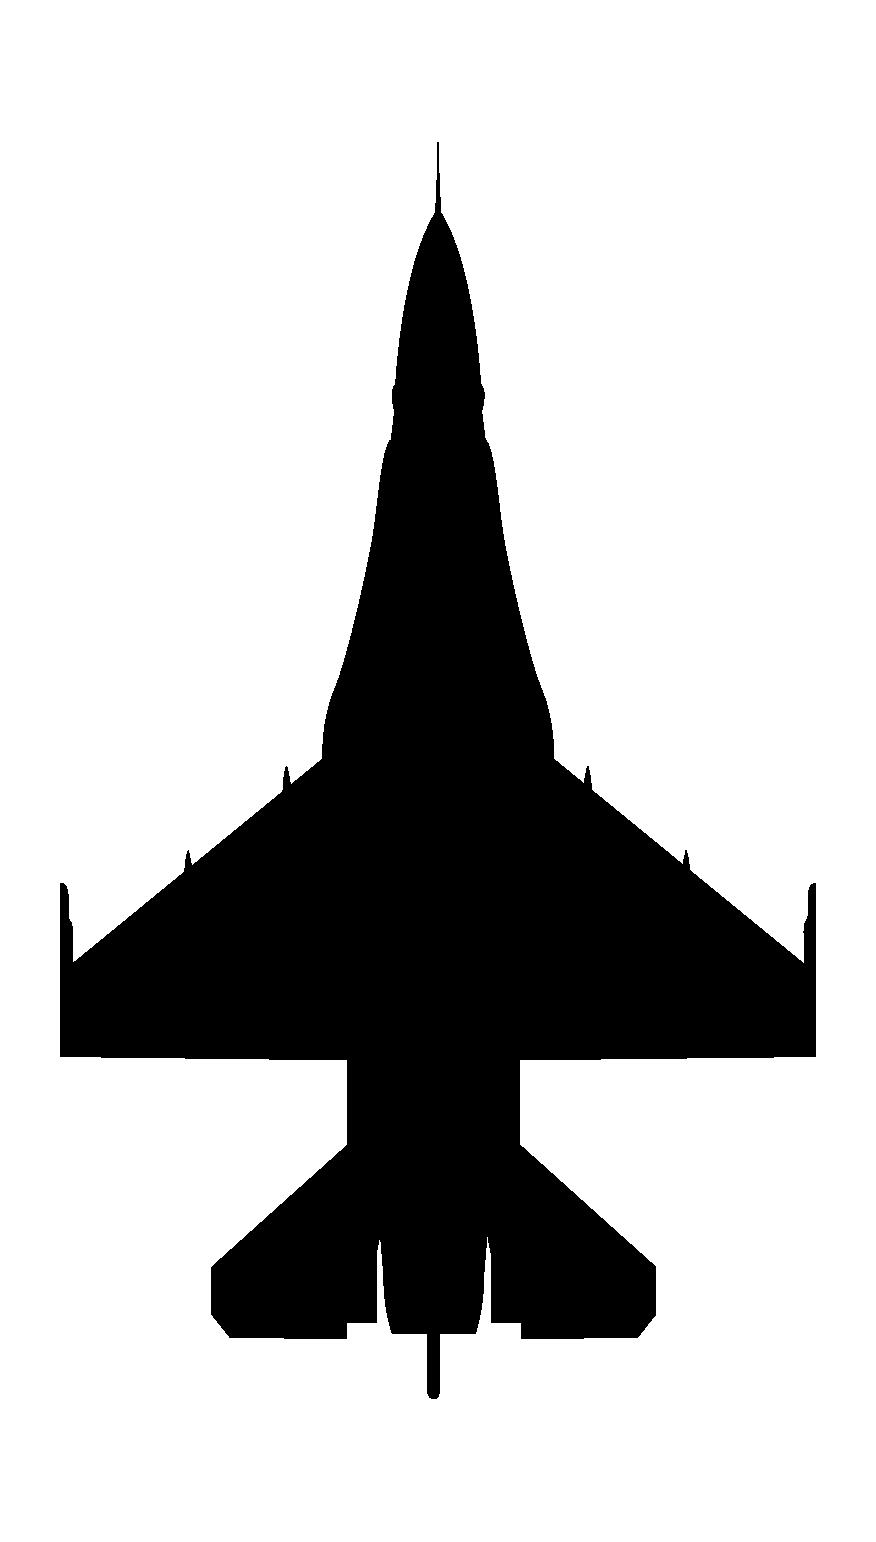
\includegraphics[
                width=7.5mm,
            ]{diagrams/aircraft/silhouette_f16_top.pdf}
        };
        
        \node[yshift=-2mm] (4fig) at (4) {
            \includegraphics[
                width=7.5mm,
            ]{diagrams/aircraft/silhouette_f16_top.pdf}
        };

        \node[anchor=north, font=\footnotesize] (1label) at (1fig.south) {1};
        \node[anchor=north, font=\footnotesize] (2label) at (2fig.south) {2};
        \node[anchor=north, font=\footnotesize] (3label) at (3fig.south) {3};
        \node[anchor=north, font=\footnotesize] (4label) at (4fig.south) {4};

    \end{tikzpicture}
    \caption{Fluid-four formation}
    \label{fig:aa_weap:form:fluidfour}
\end{figure}

\begin{figure}[htbp]
    \centering
    \begin{minipage}[b]{0.5\textwidth}
        \centering
        \begin{tikzpicture}[figstyle]
            
            \coordinate (1) at (0,0);
            \coordinate (2) at ($(1)+(-150:15)$);
            \coordinate (3) at ($(1)+(-30:15)$);
            \coordinate (4) at ($(3)+(-30:15)$);

            \node[yshift=-2mm] (1fig) at (1) {
                \includegraphics[
                    width=7.5mm,
                ]{diagrams/aircraft/silhouette_f16_top.pdf}
            };
            
            \node[yshift=-2mm] (2fig) at (2) {
                \includegraphics[
                    width=7.5mm,
                ]{diagrams/aircraft/silhouette_f16_top.pdf}
            };

            \node[yshift=-2mm] (3fig) at (3) {
                \includegraphics[
                    width=7.5mm,
                ]{diagrams/aircraft/silhouette_f16_top.pdf}
            };
            
            \node[yshift=-2mm] (4fig) at (4) {
                \includegraphics[
                    width=7.5mm,
                ]{diagrams/aircraft/silhouette_f16_top.pdf}
            };

            \node[anchor=north, font=\footnotesize] (1label) at (1fig.south) {1};
            \node[anchor=north, font=\footnotesize] (2label) at (2fig.south) {2};
            \node[anchor=north, font=\footnotesize] (3label) at (3fig.south) {3};
            \node[anchor=north, font=\footnotesize] (4label) at (4fig.south) {4};

        \end{tikzpicture}
        \caption{Fingertip formation}
        \label{fig:aa_weap:form:fingertip}
    \end{minipage}%
    \begin{minipage}[b]{0.5\textwidth}
        \centering
        \begin{tikzpicture}[figstyle]
            
            \coordinate (1) at (0,0);
            \coordinate (2) at ($(1)+(-150:20)$);
            \coordinate (3) at ($(1)+(-30:20)$);
            \coordinate (4) at ($(3)+(-150:20)$);

            \node[yshift=-2mm] (1fig) at (1) {
                \includegraphics[
                    width=7.5mm,
                ]{diagrams/aircraft/silhouette_f16_top.pdf}
            };
            
            \node[yshift=-2mm] (2fig) at (2) {
                \includegraphics[
                    width=7.5mm,
                ]{diagrams/aircraft/silhouette_f16_top.pdf}
            };

            \node[yshift=-2mm] (3fig) at (3) {
                \includegraphics[
                    width=7.5mm,
                ]{diagrams/aircraft/silhouette_f16_top.pdf}
            };
            
            \node[yshift=-2mm] (4fig) at (4) {
                \includegraphics[
                    width=7.5mm,
                ]{diagrams/aircraft/silhouette_f16_top.pdf}
            };

            \node[anchor=north, font=\footnotesize] (1label) at (1fig.south) {1};
            \node[anchor=north, font=\footnotesize] (2label) at (2fig.south) {2};
            \node[anchor=north, font=\footnotesize] (3label) at (3fig.south) {3};
            \node[anchor=north, font=\footnotesize] (4label) at (4fig.south) {4};

        \end{tikzpicture}
        \caption{Diamond formation}
        \label{fig:aa_weap:form:diamond}
    \end{minipage}
\end{figure}

\begin{figure}[htbp]
    \centering
    \begin{minipage}[b]{0.5\textwidth}
        \centering
        \begin{tikzpicture}[figstyle]
            
            \coordinate (1) at (0,0);
            \coordinate (2) at ($(1)+(-90:15)$);
            \coordinate (3) at ($(2)+(-90:15)$);
            \coordinate (4) at ($(3)+(-90:15)$);

            \node[yshift=-2mm] (1fig) at (1) {
                \includegraphics[
                    width=7.5mm,
                ]{diagrams/aircraft/silhouette_f16_top.pdf}
            };
            
            \node[yshift=-2mm] (2fig) at (2) {
                \includegraphics[
                    width=7.5mm,
                ]{diagrams/aircraft/silhouette_f16_top.pdf}
            };

            \node[yshift=-2mm] (3fig) at (3) {
                \includegraphics[
                    width=7.5mm,
                ]{diagrams/aircraft/silhouette_f16_top.pdf}
            };
            
            \node[yshift=-2mm] (4fig) at (4) {
                \includegraphics[
                    width=7.5mm,
                ]{diagrams/aircraft/silhouette_f16_top.pdf}
            };

            \node[anchor=west, font=\footnotesize] (1label) at (1fig.east) {1};
            \node[anchor=west, font=\footnotesize] (2label) at (2fig.east) {2};
            \node[anchor=west, font=\footnotesize] (3label) at (3fig.east) {3};
            \node[anchor=west, font=\footnotesize] (4label) at (4fig.east) {4};

        \end{tikzpicture}
        \caption{Trail formation}
        \label{fig:aa_weap:form:trail}
    \end{minipage}%
    \begin{minipage}[b]{0.5\textwidth}
        \centering
        \begin{tikzpicture}[figstyle]
            
            \coordinate (1) at (0,0);
            \coordinate (2) at ($(1)+(0:15)$);
            \coordinate (3) at ($(2)+(0:15)$);
            \coordinate (4) at ($(3)+(0:15)$);

            \node[yshift=-2mm] (1fig) at (1) {
                \includegraphics[
                    width=7.5mm,
                ]{diagrams/aircraft/silhouette_f16_top.pdf}
            };
            
            \node[yshift=-2mm] (2fig) at (2) {
                \includegraphics[
                    width=7.5mm,
                ]{diagrams/aircraft/silhouette_f16_top.pdf}
            };

            \node[yshift=-2mm] (3fig) at (3) {
                \includegraphics[
                    width=7.5mm,
                ]{diagrams/aircraft/silhouette_f16_top.pdf}
            };
            
            \node[yshift=-2mm] (4fig) at (4) {
                \includegraphics[
                    width=7.5mm,
                ]{diagrams/aircraft/silhouette_f16_top.pdf}
            };

            \node[anchor=north, font=\footnotesize] (1label) at (1fig.south) {1};
            \node[anchor=north, font=\footnotesize] (2label) at (2fig.south) {2};
            \node[anchor=north, font=\footnotesize] (3label) at (3fig.south) {3};
            \node[anchor=north, font=\footnotesize] (4label) at (4fig.south) {4};

        \end{tikzpicture}
        \caption{Spread formation}
        \label{fig:aa_weap:form:spread}
    \end{minipage}
\end{figure}